
% !TEX root = ../thesis.tex

\chapter{Identifying significant parameters combinations in complex
  models\label{ch:params}}


% \begin{abstract}
%   Detailed dynamical models can often be summarized in terms of only
%   a few components, reducing complexity and making exploration
%   easier and more insightful.  Pen-and-paper reduction is tedious
%   and impractical for most models, however it has the added benefit
%   of identifying parameter combinations that matter most.  Recently
%   developed frameworks computerizing model reduction leave the dual
%   aspect of effective parameter identification unaddressed,
%   relegating parameter space exploration subject to ineffective
%   sampling strategies.  Here, we lay the foundation for systematic
%   parameter reduction, rooting it in the same nonlinear data mining
%   techniques that powered model reduction in our earlier
%   equation-free framework.  Our ambition is to extend the
%   data-driven determination of effective variables by integrating
%   into it the discovery of effective model parameters.  This will
%   accelerate both dynamical simulations and parametric explorations,
%   allowing us to efficiently map out the behavior of complex models.

% \end{abstract}

Our motivation for this paper is the work of Sethna and others on
parameter reduction\cite{AS06}, as well as similar ideas and studies
on non-identifiability \cite{RKMBSKT09} and active subspaces
\cite{CDW14}. These authors investigate the widespread phenomenon in
which large ranges of model parameters produce nearly constant model
predictions. This behavior, termed parameter sloppiness, has been
identified in complex models arising in a wide range of fields.

One extreme case arises when model predictions depend solely on some
reduced number of parameters or parameter combinations.  In such a
setting, the parameter space is foliated by lower-dimensional sets
across which those combinations, and hence also the observables,
retain their value; Fig.~\ref{fig:non-id} depicts one such case.
Under those circumstances, it is neither possible nor desirable to
infer parameter values from observations; the parameters are said to
be non-identifiable. Instead, one should re-parameterize the model
with a reduced number of \emph{identifiable, effective parameters}.
Although such identifiability analysis decomposes parameter space
globally on the basis of model response, that decomposition is often
trivial and certainly non-robust, as models typically respond (if only
weakly) to all parameter variations.  Sensitivity analysis is more
robust, as it weighs the degree by which parameter combinations affect
response, but it only operates locally in parameter space as it is
inherently linear. We reconcile and fuse these two perspectives here
into an entirely data-driven framework for the identification of more
global effective parameters.

\begin{figure}
  \centerline{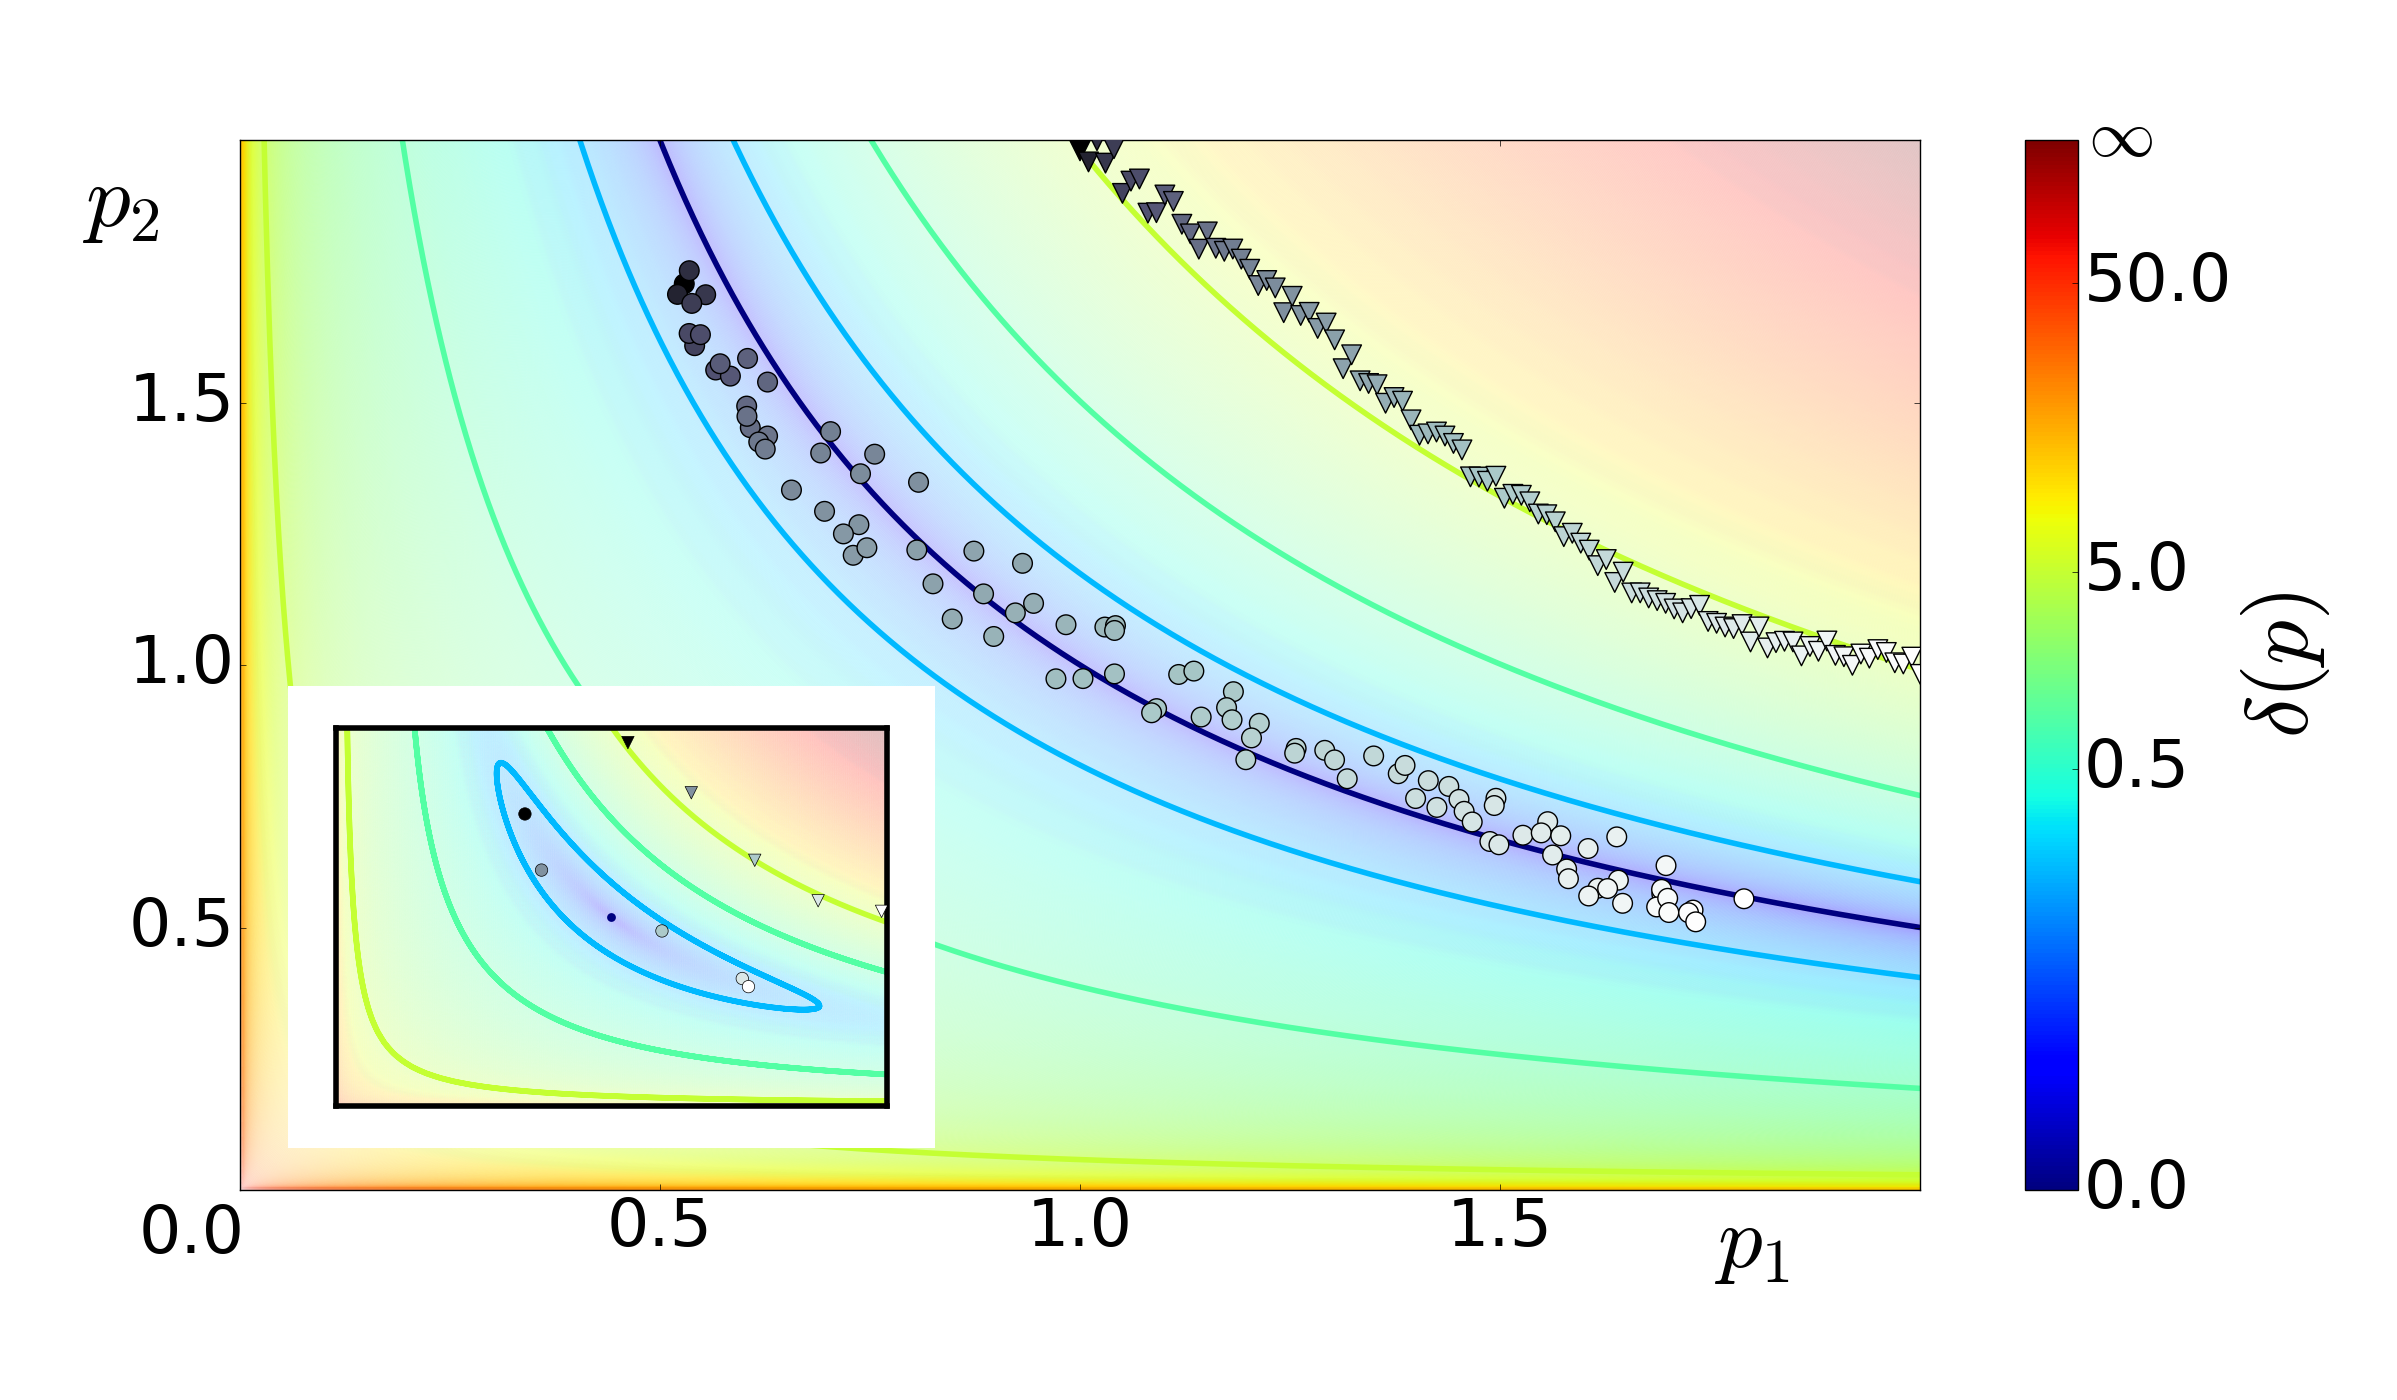
\includegraphics[width=1.0\linewidth]{p2-p1}}
  \caption[Illustration of effects of sloppiness on optimization]{Global foliation of parameter space for the model
    $\mathbf{f}(p_1,p_2) = (p_1 p_2 , \ln(p_1) + \ln(p_2) , (p_1 p_2)^2)$.
    Level sets of the effective parameter $p_\mathrm{eff} = p_1 p_2$
    can be learned by fitting parameter values to specific data.
    To demonstrate, we fed the data $\mathbf{f}^*=(1,0,1)$ and various initializations 
    to a gradient descent algorithm, approximately obtaining the hyperbola $p_1 p_2 = 1$ (colored by initialization).
    \label{fig:non-id} }
\end{figure}

Consider the model presented in Fig.~\ref{fig:non-id}, consisting of a
vector function of two parameters,
$\mathbf{f}(p_1,p_2) = (p_1 p_2 , \ln(p_1) + \ln(p_2) , (p_1 p_2)^2)$.
If we only have input--output information (black-box function
evaluators) and no explicit formulas, we cannot immediately establish
that it is only the single parameter $p_\mathrm{eff}=p_1 p_2$ that
matters.  Trying to fit the model to observations $\mathbf{f}^*$, one
would then be surprised to find that an entire curve in parameter
space fits the observations.  An optimizer based only on function
evaluations would also be ``confused.''  For a practical fitting
tolerance $\delta\approx10^{-3}$, a curve of different initializations
would converge through steepest descent to many different results
within the band shown in the figure.  The ``good'' parameter set is
clearly effectively one-dimensional; more importantly, beyond this
particular fit to particular data, the entire parameter space is
foliated by such one-dimensional curves of indistinguishable, from the
model response perspective, parameter values.  Parameter
non-identifiability is a structural feature of the model, not germane
to optimization.  The ``appropriate,'' \emph{intrinsic} way to
describe parameter space for this problem is through the single
effective parameter $p_\mathrm{eff}=p_1 p_2$ and its level sets.

Consider now the situation in the inset of Fig.~\ref{fig:non-id} for
the perturbed model $\mathbf{f}^\epsilon$, where the parameters \emph{are}
identifiable and minimizers unique: a perfect fit now exists.
However, the foliation in Fig.~1a is remembered in the shape of the
residual level curves and the optimizer is equally confused in
practice.  It is the confusion of the optimizer that provided one of
the original motivations in Sethna's work.  This model is sloppy, in
Sethna's terminology, and clearly sloppiness goes beyond
non-identifiability.

A fundamental insight is that the presence of effectively
lower-dimensional neutral sets, such as the thick curves seen in
Fig.~\ref{fig:non-id}, reduces the number of parameters affecting the
system.  Our goal is to extract the ``appropriate,'' intrinsic
parameterization of the input (parameter) space from input--output
data.  As we shall see, this parameterization may vary across input
space regimes.  We will show how this variation can be associated with
the traditional notions of regular and singular perturbations in
explicit models when the number of effective parameters changes.


% Linear problem no delta model manifold two parameters regimes
% --------------Bound to Bound Frenklach --- parenthesis --- from one
% to zero dimensions this way we see that model reduction is a sub
% case of sloppiness

% add the delta regular perturbations


% ----------

% Henon sloppiness in the eye of the beholder THIS COULD BE THE LAST
% THING: gauge invariant data mining....

% ---------

% DMAPS

% Start on the good set -- get dimensionality and parametrization of
% good set

% NOW FULL SPACE ** use manifold metric -- two parameters, one
% effective - WORKS ** is this enough ? no, see example (one to one)
% ** need mixed kernel -- SHOW same above -- WORKS ** the Mahalanobis
% - show it on Henon ** Here point out gauge invariance...


% -------------






% ABC we know QSSA - regime where reduces and HOW it reduces(effective
% parameters) can we recapture this with data show that yes DO WE FIND
% ANYTHING MORE ???  there is an OBVIOUS QSSA --- and a PROFESSIONAL
% QSSA (paper and pencil done) and we can see that the data does the
% Professional QSSA

% ---------

% MM setup (what we measure) -- "Good" (=transformed) parameters ->
% eps is singularly perturbed -> kappa is regularly perturbed (=> 5->3
% parameters) -> ST non-sloppy -> one effective parameter keff(VM,KM)
% -- "Bad" (=original) parameters -> ST non-sloppy (but experimentally
% measured) -> 1 effective parameter keff(k(-1),k1,k2) [normally would
% expect 2, but sloppiness in VM,KM reduced by one more] -> Connection
% to ABC and keff(ABC) -- Something standard -- Something non-standard
% we knew -- Something non-standard we did not know but falls out of
% data


% QSSA (what we expect to find - what is the effective parameter)


% DISCUSSION

% quick summary level sets - WILL ? - extension - ABC Geom Harmonics,
% David, Andrew ...  optimization - search in good directions

% `bottom line- it is all in the metric and the culmination is gauge



% ------------------------------------------------

\section{Sloppiness in parameters and initial conditions}

To fix ideas and definitions, we start with a dynamical model
% 
\begin{equation}
  \dot{\mathbf{x}}(t \vert \mathbf{p})
  =
  \mathbf{v}(\mathbf{x} \vert \mathbf{p}) ,
  \ \mbox{where} \
  \dot{\mathbf{x}}
  =
  \frac{d\mathbf{x}}{dt}
  \ \mbox{and} \
  \mathbf{x}(t_0 \vert \mathbf{p}) = \mathbf{x}_0(\mathbf{p}) .
  \label{x'=v}
\end{equation}
% 
The vector $\mathbf{x}(t \vert \mathbf{p}) \in \mathbb{R}^d$ collects
the state variables, also called just "variables", at time $t$ that
correspond to the vector field
$\mathbf{v} : \mathbb{R}^d \times \mathbb{R}^M \to \mathbb{R}^d$, to
the parameter settings $\mathbf{p} \in \mathbb{R}^M$ and to the
initial state $\mathbf{x}_0(\mathbf{p})$.  The \emph{output} of
\eqref{x'=v} is the system state $\mathbf{x}(t \vert \mathbf{p})$ for
all times $t>t_0$, written $\mathbf{x}(\cdot\vert\mathbf{p})$, but
\emph{data} are only partial observations of that time course.
Observing the system means recording a number $N \ge M$ of outputs
into an $N-$tuple $\mathbf{f}(\mathbf{p}) \in \mathbb{R}^N$, for fixed
settings $\mathbf{p}$.  Each setting $\mathbf{p}$ yields a
well-defined \emph{model response} $\mathbf{f}(\mathbf{p})$ and, as
$\mathbf{p}$ moves in parameter space, $\mathbf{f}(\mathbf{p})$ traces
out a (generically $M-$dimensional) output manifold $\mathcal{M}$ in
data space $\mathbb{R}^N$.  We will be writing
$\mathcal{M}-$\emph{manifold} to conform with the ``model manifold''
term in \cite{TMS}.

% By observation we understand \emph{quantification} through a set of
% measurement functions $f_1,\ldots,f_N$ transforming the time course
% into numbers, so that data have the form
%% 
% \begin{equation}
%   \mathbf{f}(\mathbf{p})
% %   =
% %   \big[
%   f_1(\mathbf{x}(\cdot\vert\mathbf{p})) \, ,
% %   \ldots \, ,
%   f_N(\mathbf{x}(\cdot\vert\mathbf{p}))
% %   \big]
% %   \in
%   \mathbb{R}^N .
%   \label{f(x)}
% \end{equation}
%% 
% This maps parameter values $\mathbf{p}$ to a point in data space
% $\mathbb{R}^N$ through the mediation of the time course
% $\mathbf{x}$.  across a domain in $\mathbb{R}^M$

Fig.~\ref{fig:sing-pert} shows the $\mathcal{M}-$\emph{manifold} for
the prototypical singularly perturbed model
% 
\begin{equation}
  \dot{x} = -x/\varepsilon, \quad
  x(0) = x_0 .
  \label{1D-model-singpert}
\end{equation}
For this system, we view both $\varepsilon$ and $x_0$ as parameters
and monitor $x$ at distinct times $0 < t_1 < t_2 < t_3$, so that
% 
\begin{equation}
  \mathbf{p} = (\epsilon , x_0)
  \quad\mbox{and}\quad
  \mathbf{f}(\mathbf{p})
  =
  \big[
  x(t_1 \vert \mathbf{p}) \, ,
  x(t_2 \vert \mathbf{p}) \, ,
  x(t_3 \vert \mathbf{p})
  \big] . 
  \label{1D-pf}
\end{equation}
% 
% Sliding down $\mathcal{M}$ in the plot amounts to decreasing $\epsilon$
% and increasing $x_0$.
In the spirit of the bound-to-bound approach by Frenklach and
co-workers, it is instructive to compare side by side how boundaries
on the $\mathcal{M}-$manifold map to parameter space and vice versa.
Fig.~\ref{fig:sing-pert} shows several nested subdomains of the
$\mathcal{M}-$manifold created by intersecting that manifold with
concentric spheres, that is, the domains
$\|\mathbf{f}(\mathbf{p}) - \mathbf{f}(\mathbf{p}^*)\| \le \delta$
with $\mathbf{f}(\mathbf{p}^*)$ the center and for various tolerances
$\delta$.  The smallest, dark blue boundary is fully contained in the
manifold interior and maps to a compact, ellipse-like subset of
parameter space: all settings inside it yield responses within the
smallest tolerance.  That preimage grows with $\delta$ and eventually
becomes unbounded (light blue boundary) when the subdomain becomes
tangent to the $\mathbf{f}_1-$axis (boundary~B), with the point of
tangency mapping to infinity on the parameter plane.  Even larger
boundaries are only partly contained in the $\mathcal{M}-$manifold and
their preimages also unbounded, with the one tangent boundary~A
extending to $\varepsilon=0^+$ (orange boundary).

This manifests that boundaries of the $\mathcal{M}-$manifold
correspond to asymptotic regimes themselves \cite{TQ}, namely
$\varepsilon \gg t_3$ for A and $\varepsilon \ll t_1$ for B or, for
fixed observation times, $\varepsilon \to \infty$ and
$\varepsilon \to 0$.  As a result,
$\mathbf{f}(\mathbf{p}) = (x_0,x_0,x_0)$ for $\varepsilon \to \infty$,
so that boundary~A is parameterized by the initial condition $x_0$
alone: the model output becomes \emph{sloppy} in $\epsilon$ and
one-dimensional.  The regime $\varepsilon \to 0$, on the other hand,
corresponds to a singularly perturbed problem, with boundary~B
parameterized by
$x(t_1 \vert \mathbf{p}) = x_0\mathrm{e}^{-t_1/\varepsilon}$.  In that
regime, $x(t_1 \vert \mathbf{p})$ converges to the origin for finite
$x_0$, so that our system effectively becomes zero-dimensional.  Had
such a singular perturbation occurred in the context of a larger
system of differential equations, we would have been able to reduce
the number of state variables needed to describe our system.  hence,
by including initial conditions as model parameters, we can
effectively find possible reductions in both parameter- and
state-space.  Another important observation is that the qualitative
features of the $\mathcal{M}-$manifold are model features, independent
of parameter inference and fitting (subdomains) and relating to
working in the vicinity of an $\mathcal{M}-$manifold boundary.
Clearly, grouping different system outputs into $\mathbf{f}$ would
give α different $\mathcal{M}-$manifold.

\begin{figure*}
  \centering
  \begin{subfigure}[t]{0.45\linewidth}
    \centering
    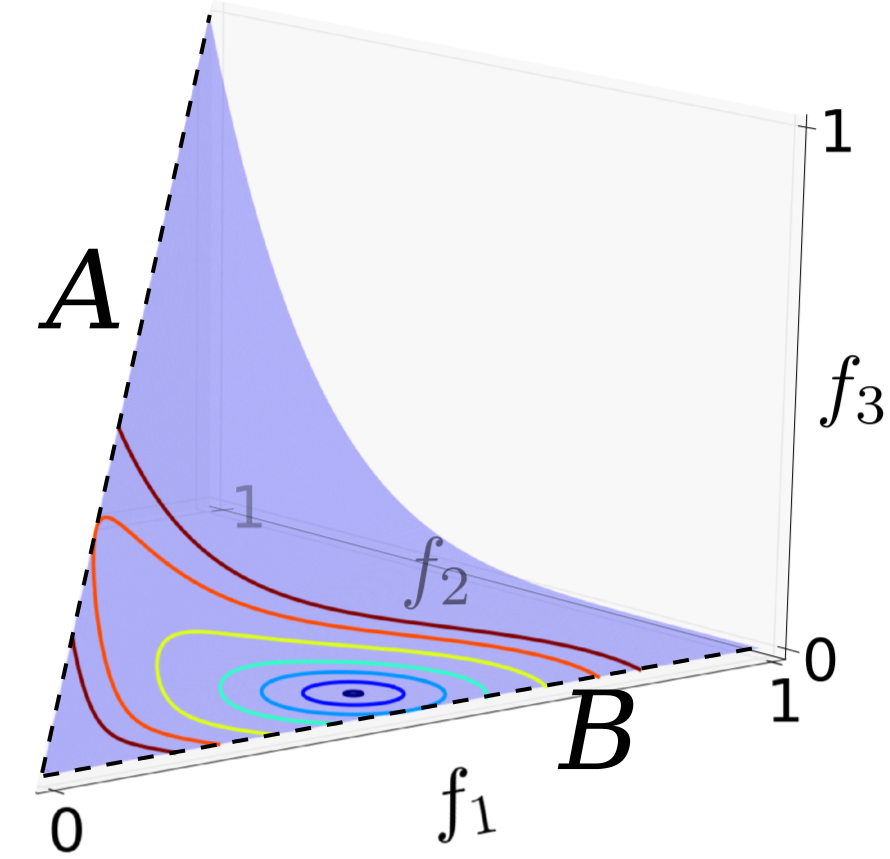
\includegraphics[height=2in]{f3-f2-f1-delta-cropped}
    \subcaption{Model manifold with overlaid contour lines for
      $\delta$ equal to $0.01$, $0.06$, $0.10$, $0.14$, $0.22$, $0.28$
      and $0.34$.  Boundary~A ($f_1 = f_2 = f_3$) marks the regime
      $\epsilon \rightarrow \infty$ and boundary~B ($f_2 = f_3 = 0$)
      the regime $\epsilon \rightarrow0$.
      \label{fig:sing-pert-mm} }
  \end{subfigure}
  \hspace{0.5cm}
  \begin{subfigure}[t]{0.45\linewidth}
    \centering
    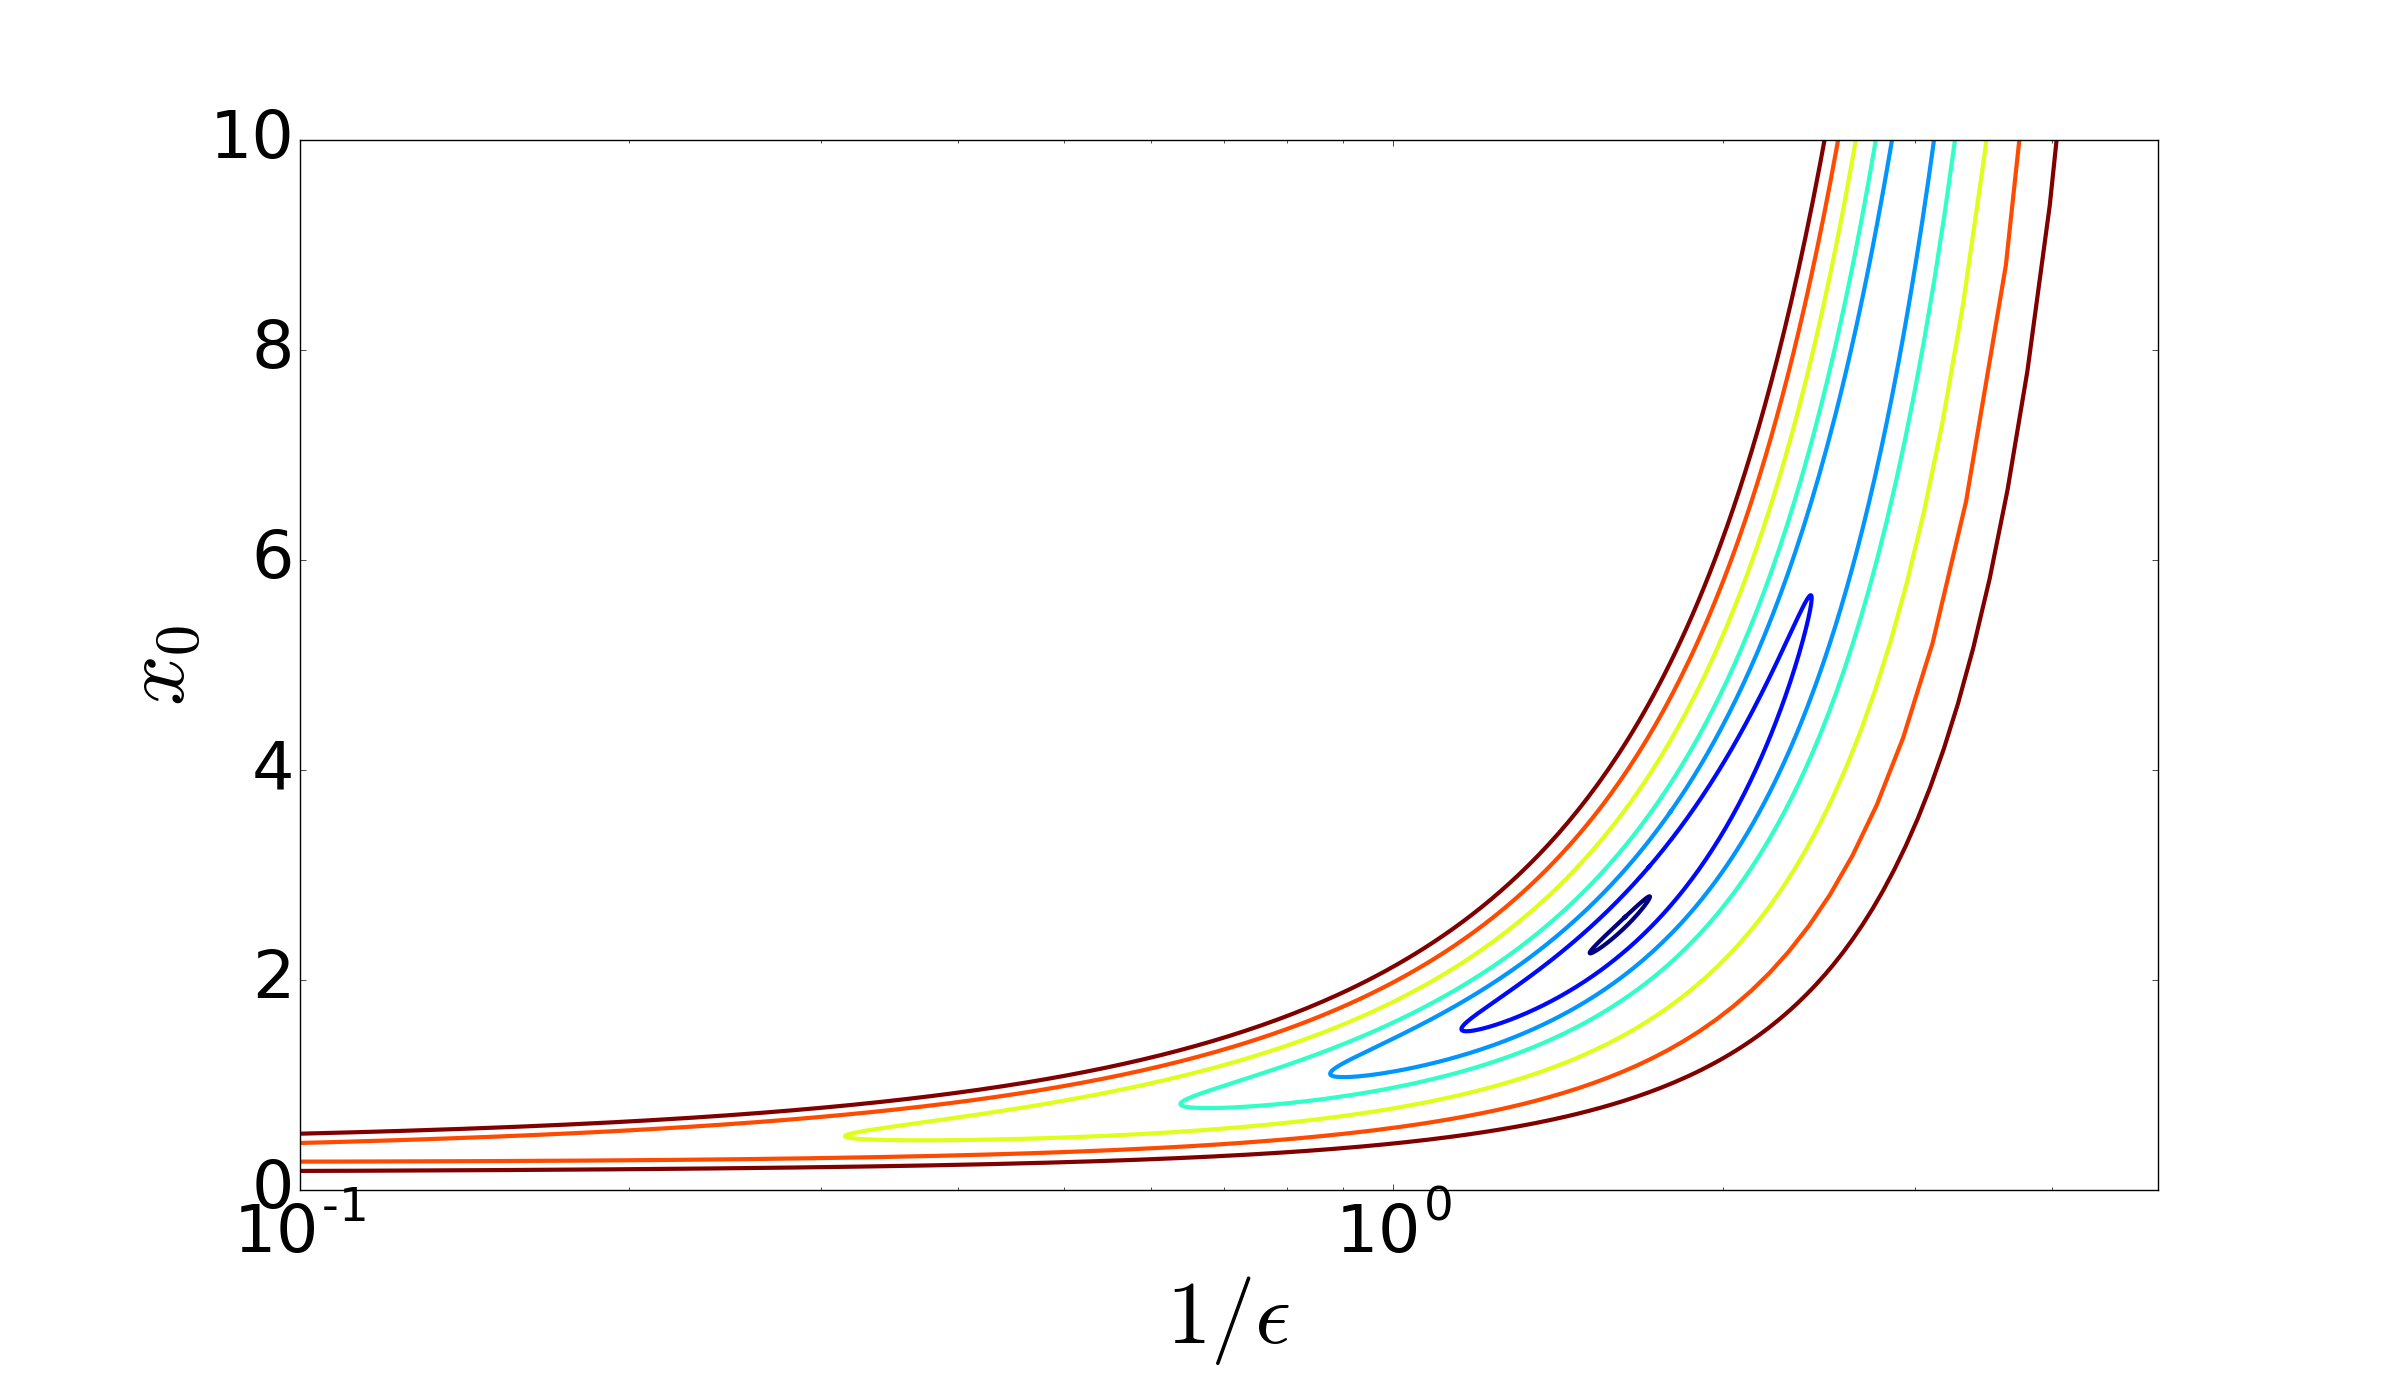
\includegraphics[width=1.0\linewidth]{x0-eps-delta-singpert}
    \subcaption{Parameter space of the singularly perturbed system
      with contour lines from left figure for $\delta$ equal to
      $0.01$, $0.06, 0.10, 0.14, 0.22, 0.28, 0.34)$. At the light blue
      curve which intersects the $f_1$ axis, the curve opens up to the
      right as $\epsilon \rightarrow 0$, while at the light red curve
      which intersects the $f_1 = f_2 = f_3$ line, the contour also
      opens up towards the left as $\epsilon \rightarrow
      \infty$. \label{fig:sing-pert-params} }
  \end{subfigure}
  \caption[Model manifold and parameter space of the singularly
    perturbed system]{Model manifold and parameter space of the singularly
    perturbed system \eqref{1D-model-singpert} with select $\delta$
    contours.
    \label{fig:sing-pert} }
\end{figure*}
% 

We conclude this section by contrasting regular to singular
perturbations through the equally simple model
% 
\begin{equation}
  \dot{x} = -\epsilon x^3 - x,
  \quad
  x(0) = x_0 ,
  \label{1D-model-regpert}
\end{equation}
% 
with $\mathbf{p}$ and $\mathbf{f}$ as above.  Fig.~\ref{fig:reg-pert}
shows the model manifold and the parameter plane, with the plotted
contours bounding regions of increasing $\delta$.  These countours
extend to $\varepsilon = 0^+$ past a certain $\delta$, illustrating
that the model becomes sloppy for small $\epsilon$ but retains its strong
dependence on $x_0$.  In regular perturbations, loss of parameters
occurs without concomitant loss of variables: the model parameters can
be simplified but the number of variables cannot be reduced.

\begin{figure*}
  \centering
  \begin{subfigure}[t]{0.45\linewidth}
    \centering
    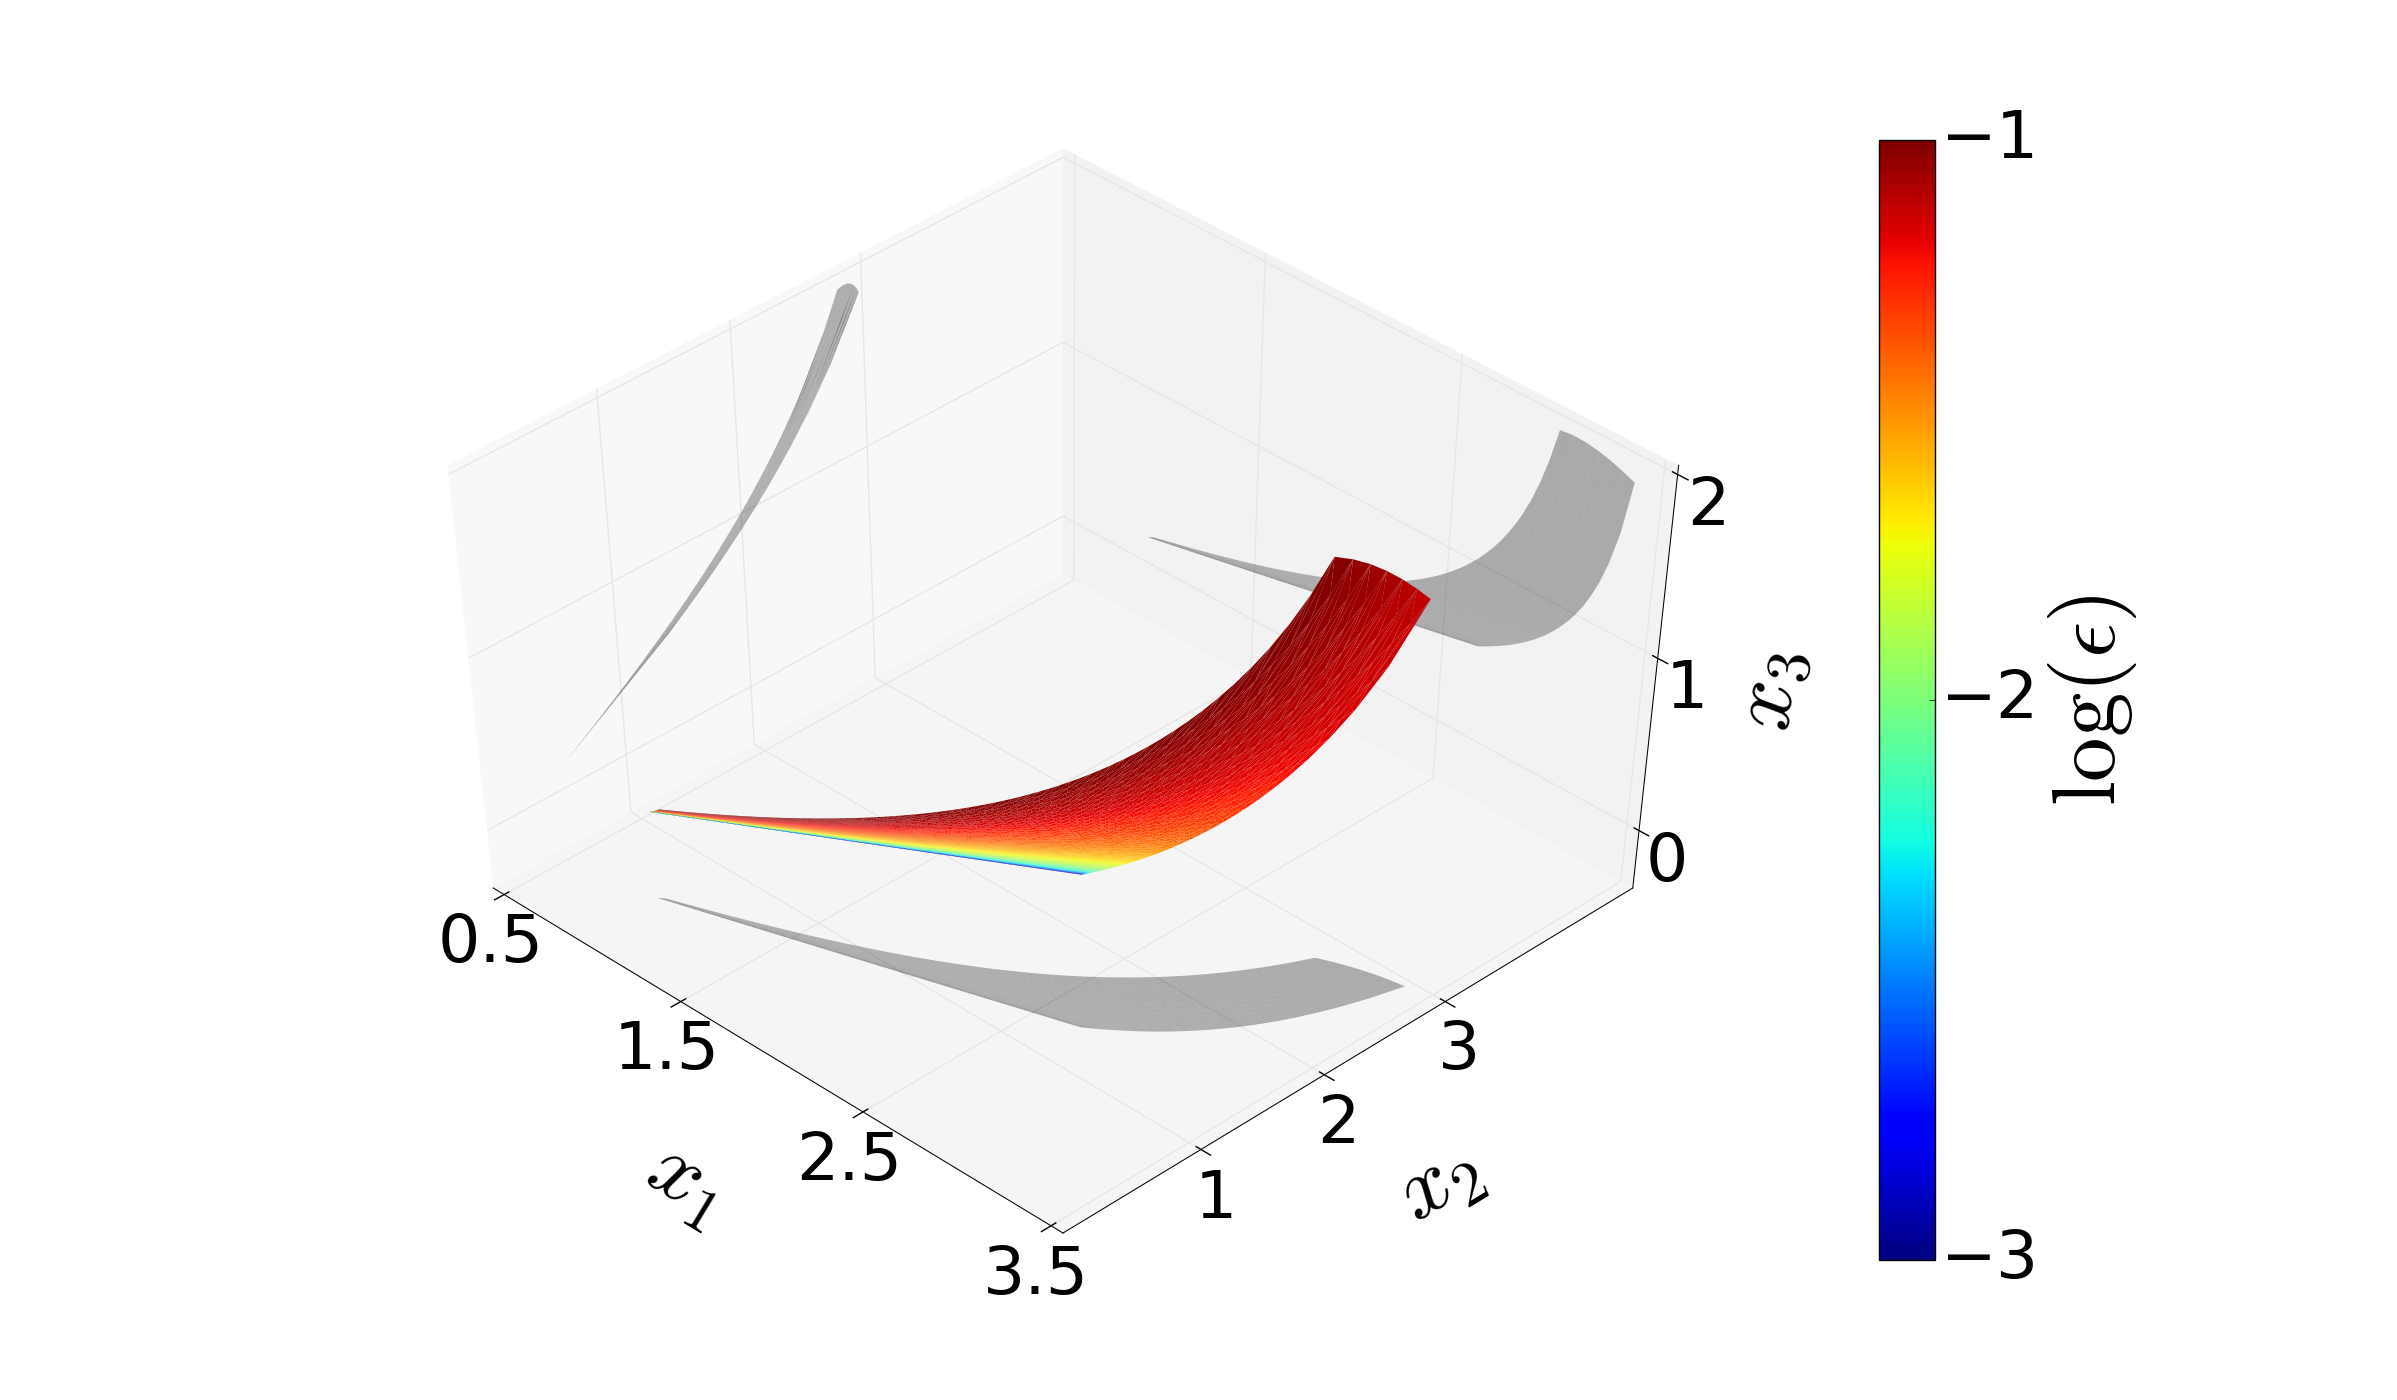
\includegraphics[width=\linewidth]{x3-x2-x1-eps}
    \caption{Model manifold of regularly perturbed system with
      parameters $x_0$ and $\epsilon$, colored by $\epsilon$. As
      $\epsilon$ decreases, the model response is increasingly
      determined solely by $x_0$ as the system converges to
      $x' = x^3$. \label{fig:reg-pert} }
  \end{subfigure}
  \hspace{0.5cm}
  \begin{subfigure}[t]{0.45\linewidth}
    \centering
    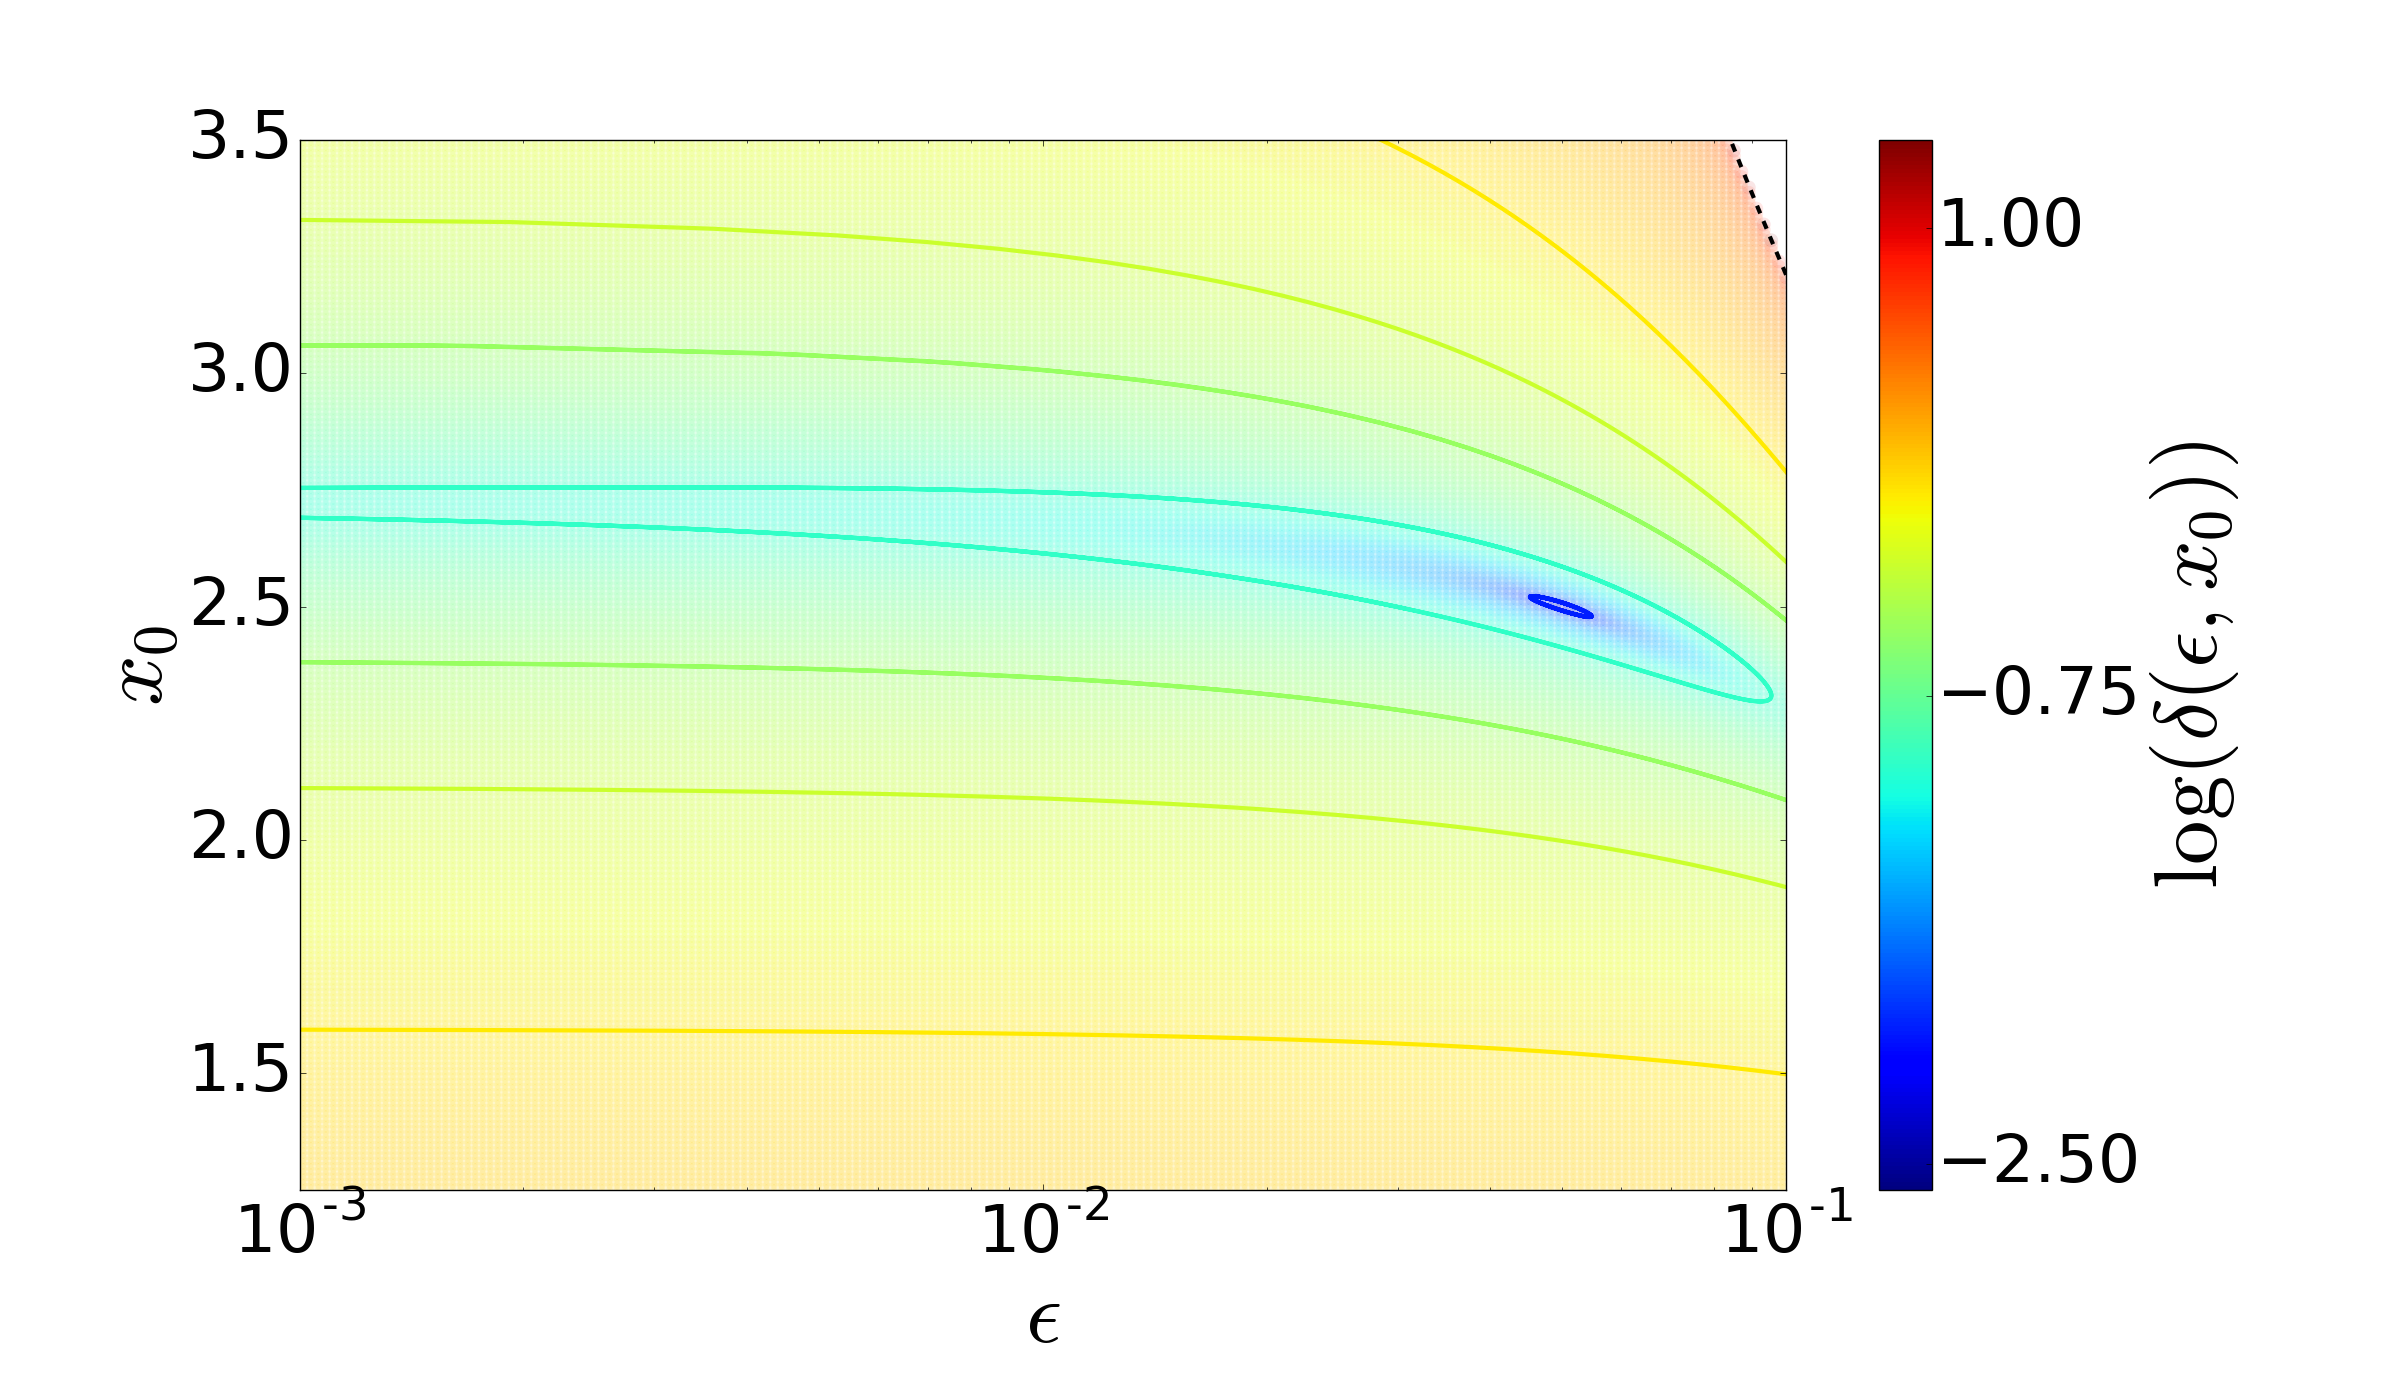
\includegraphics[width=\linewidth]{x0-eps-delta}
    \subcaption{Parameter plane of the regular perturbation system
      colored by $\delta^2$, the distance from the base parameter
      values at $x_0^*$ and $\epsilon^*$. For larger $\epsilon$ both
      $\epsilon$ and $x_0$ affect the value of $\delta$, while
      $\delta$ flattens horizontally along the $\epsilon$ axis at
      small $\epsilon$, only varying in the one remaining important
      parameter direction: $x_0$. \label{fig:reg-pert-params} }
  \end{subfigure}
  \caption[Model manifold and parameter space of the regularly
  perturbed system]{Model manifold and parameter space of the
    regularly perturbed system \eqref{1D-model-regpert} with select
    $\delta$ contours \label{fig:reg-pert} }
\end{figure*}

\begin{figure*}[ht!]
  \centering
  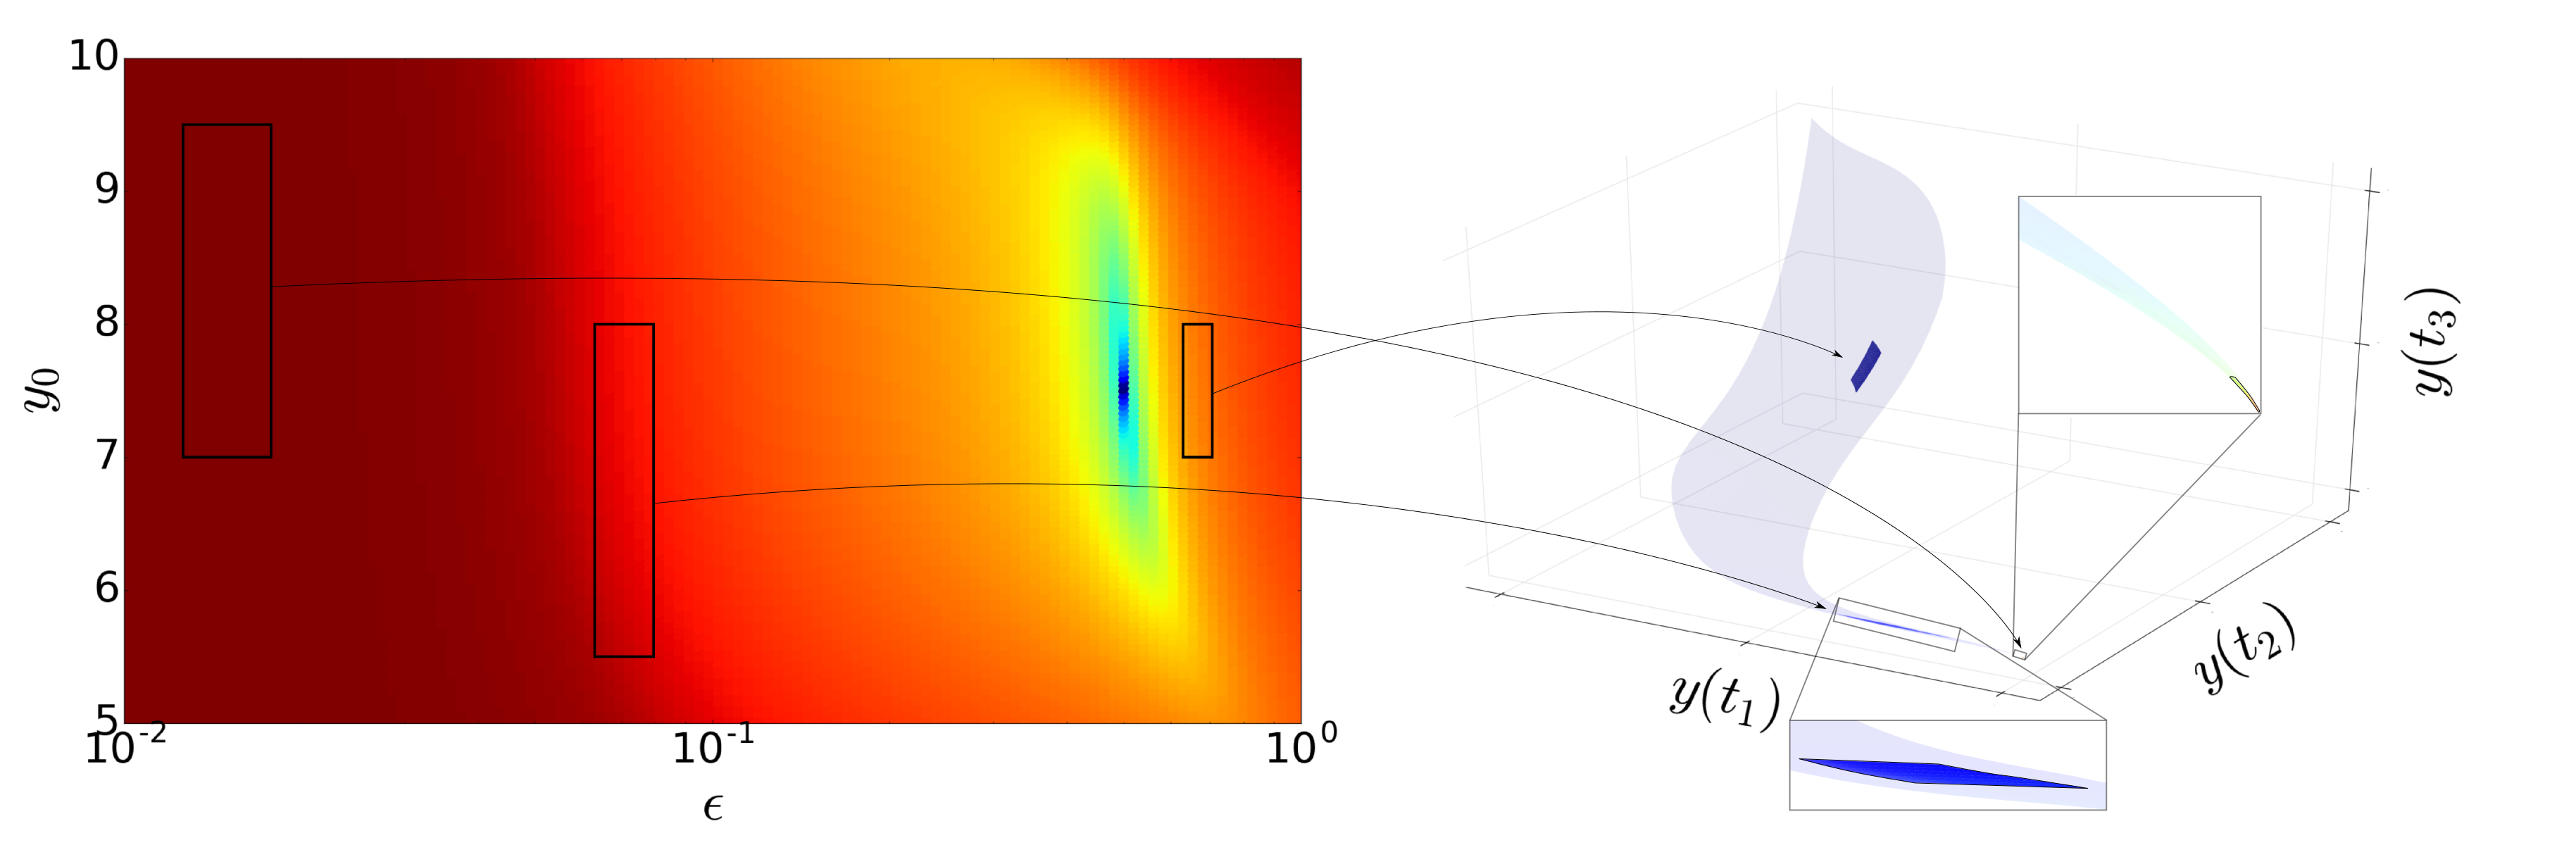
\includegraphics[width=\textwidth]{mm-combined}
  \caption[Quantitative illustration of mapping from parameter space
  to the model manifold]{Correspondence between parameter space (left)
    and the model manifold (right). At large values of $\epsilon$,
    rectangles in parameter space are mapped to skewed rectangles on
    the model manifold. At intermediate values of $\epsilon$, they are
    stretched into nearly one-dimensional segments. At small values
    where the system is singularly perturbed, patches in parameter
    space map to approximately the same point on the model manifold,
    the hallmark of sloppiness.}
\end{figure*}

\section{Parameter inference}

Parameter sloppiness builds on the observation that different
parameter perturbations can affect the generated data drastically
differently, despite the existence of a one-to-one correspondence
between data and parameters.  This is already reflected in eigenvalue
disparities in an SVD of the Jacobian
$D_\mathbf{p}\mathbf{f}(\mathbf{p})$, with small eigenvalues tied to
\emph{sloppy parameter directions} that hardly affect the data.
Although Jacobian-based sensitivity analysis is local, the footprint
of sloppiness is the existence of \emph{extended} regions in parameter
space evoking nearly identical data.  Such neutral sets are
effectively lower-dimensional and roughly foliate full-dimensional
regions of parameter space, with effective system parameters remaining
approximately constant on them.

% Finally, we note that sloppiness is an open property of the input--output system characterizing entire regimes in input space and often linked with manifold boundaries.\\

In the context of the perturbed model corresponding to
Fig.~\ref{fig:non-id}, an $M-$dimensional ball around
$\mathbf{f}^*=(1,0,1)$ is pulled back to an ellipsoid centered at
$\mathbf{p} = (1,1)$ with widely disparate principal axes.  The
largest principal directions correspond to sloppy parameter
combinations, and they can be unraveled by linear algebraic techniques
such as Principal Component Analysis.  In reality, pronounced
deviations of \eqref{1D-model-singpert} from linearity mean that
neighborhoods of $\mathbf{f}^*$ are mapped to curved neutral sets in
parameter space with disparate characteristic length scales; this is
already evident in Fig.~\ref{fig:sing-pert}.  Such neutral sets are
not directly amenable to linear techniques, requiring instead the
development of a nonlinear data mining framework to identify them and
the associated effective parameters.  We will make these ideas
concrete below through a series of examples.

\section{Visualizing nonlinear sloppiness}
The classical technique to analyze parameter sensitivity is through
analysis of the singular values of the Jacobian
$D_\mathbf{p}\mathbf{f}(\mathbf{p})$.  Large disparities suggest
directions in parameter space along which the model response
$\mathbf{f}$ remains essentially constant.  Due to its local nature,
this technique fails to uncover parameter sloppiness or yields
misleading results if there are strong nonlinearities present in the
effective parameter set. We review a few illustrative examples
directly below.

\subsection{Creating sloppiness} \label{sec:hm} Consider a
prototypical nonlinear ODE model crafted from the linear system

\begin{align}
  \begin{aligned}
    X' &= -\lambda X , \\
    \epsilon Y' &= -Y ,
    \label{eqn:sp}
  \end{aligned}
\end{align}

by passing to new state space coordinates given implicitly by
$(X, Y) = (x-\beta y^2 , y - \alpha x^2)$.  The result is a nonlinear
but tractable ODE model with parameters
$\alpha,\beta,\lambda,\epsilon$.  For reasons of illustration, we set
$\mathbf{p} = (\alpha,\lambda)$, keeping $\beta$ and $\epsilon$ fixed at
$10^{-2} and 10^{-3}$ with $\epsilon \ll \lambda$.  In that regime,
the ODE system is singularly perturbed with a slow manifold
$y = a x^2$ that attracts each initial conditions $(x_0,y_0)$ in a
neighborhood of the origin along the fast fiber
$x = b y^2 + x_0 - b y_0^2$.  We set the model response to
\begin{align}
  \mathbf{f}^*(\mathbf{p}) = \begin{bmatrix} x(t_1;\mathbf{p}) , \cdots , x(t_{N};\mathbf{p}) , y(t_1;\mathbf{p}) , \cdots , y(t_{N};\mathbf{p}) \end{bmatrix}^\mathrm{T} ,
\end{align}
for some number $N=5$ and times evenly spaced in $t \in [0.5, 2.5]$.
The parameters $\alpha$ and $\lambda$ control the curvature of and
slow decay on the slow manifold, and neither is sloppy
(Fig.~\ref{fig:henon}, right panel).  The situation might nevertheless
appear entirely different once transformed parameters are introduced.
Using the contrived but illustrative map
$\mathbf{p} = (u_4(\alpha,\lambda), w_4(\alpha,\lambda)$, where
$(u_4,w_4)$ is the fourth iteration of the H\'{e}non map
\begin{align}
  \begin{aligned}
    u_{n+1} &= 1 - \gamma u_n^2 + w_n , \\
    w_{n+1} &= \zeta u_n ,
    \label{eqn:henon}
  \end{aligned}
\end{align}
yields a new parameter set that is in one-to-one correspondence with
the original one but highly nonlinear.  Sloppiness is here pronounced
(Fig.~\ref{fig:henon}, left panel), with the neutral set being
elongated, bent and folded.  Again, we stress that one cannot know
\textit{a priori} the structure of the parameter space.  All one has
is two ``knobs'' tuning the system, and the existence of the parameter
set $(\alpha,\lambda)$ is not known in advance.

To investigate the structure of the neutral sets corresponding to some
reference model response $\mathbf{f}^*$, we sampled $\mathbf{p}$
uniformly on the rectangle $(-2, 30) \times (-1.5, 0.7)$, recording
for each sample the response $\mathbf{f}(\mathbf{p})$ it generates and
the associated squared Euclidean distance
$\delta(\mathbf{p}) = \| \mathbf{f}(\mathbf{p}) - \mathbf{f}^* \|^2$
from the reference response $\mathbf{f}^*$.  In the absence of noise,
i.e. for perfect measurements $\mathbf{f}(\mathbf{p})$, $\delta$ has a
unique minimum at $\mathbf{p}^*$.  Fig.~\ref{fig:henon} shows the
sampled values that yield $\delta<0.4$, colored by their
$\delta-$value, both in $\mathbf{p}-$ and in $(\alpha,\lambda)-$space.
The nonlinear character of the model is evident in the deviation of
the neutral set from an elliptical shape, mild in the
$(\alpha,\lambda)-$space and overpronounced in $\mathbf{p}-$space.

The significance of this example is twofold.  First, parameter
sloppiness may be accompanied by nonlinearities in the underlying
model that invalidate traditional sensitivity analysis.  Second, we
see that this phenomenon is really a result of a poorly parameterized
model, which an appropriate re-parameterization can largely
ameliorate.  This suggests two approaches to address model sloppiness:
develop techniques capable of handling nonlinearity and work with the
original, nonlinear model, or develop techniques to directly remove
the nonlinearity from the model.  This paper takes the former
approach.

\begin{figure*}[ht!]
  \centering
  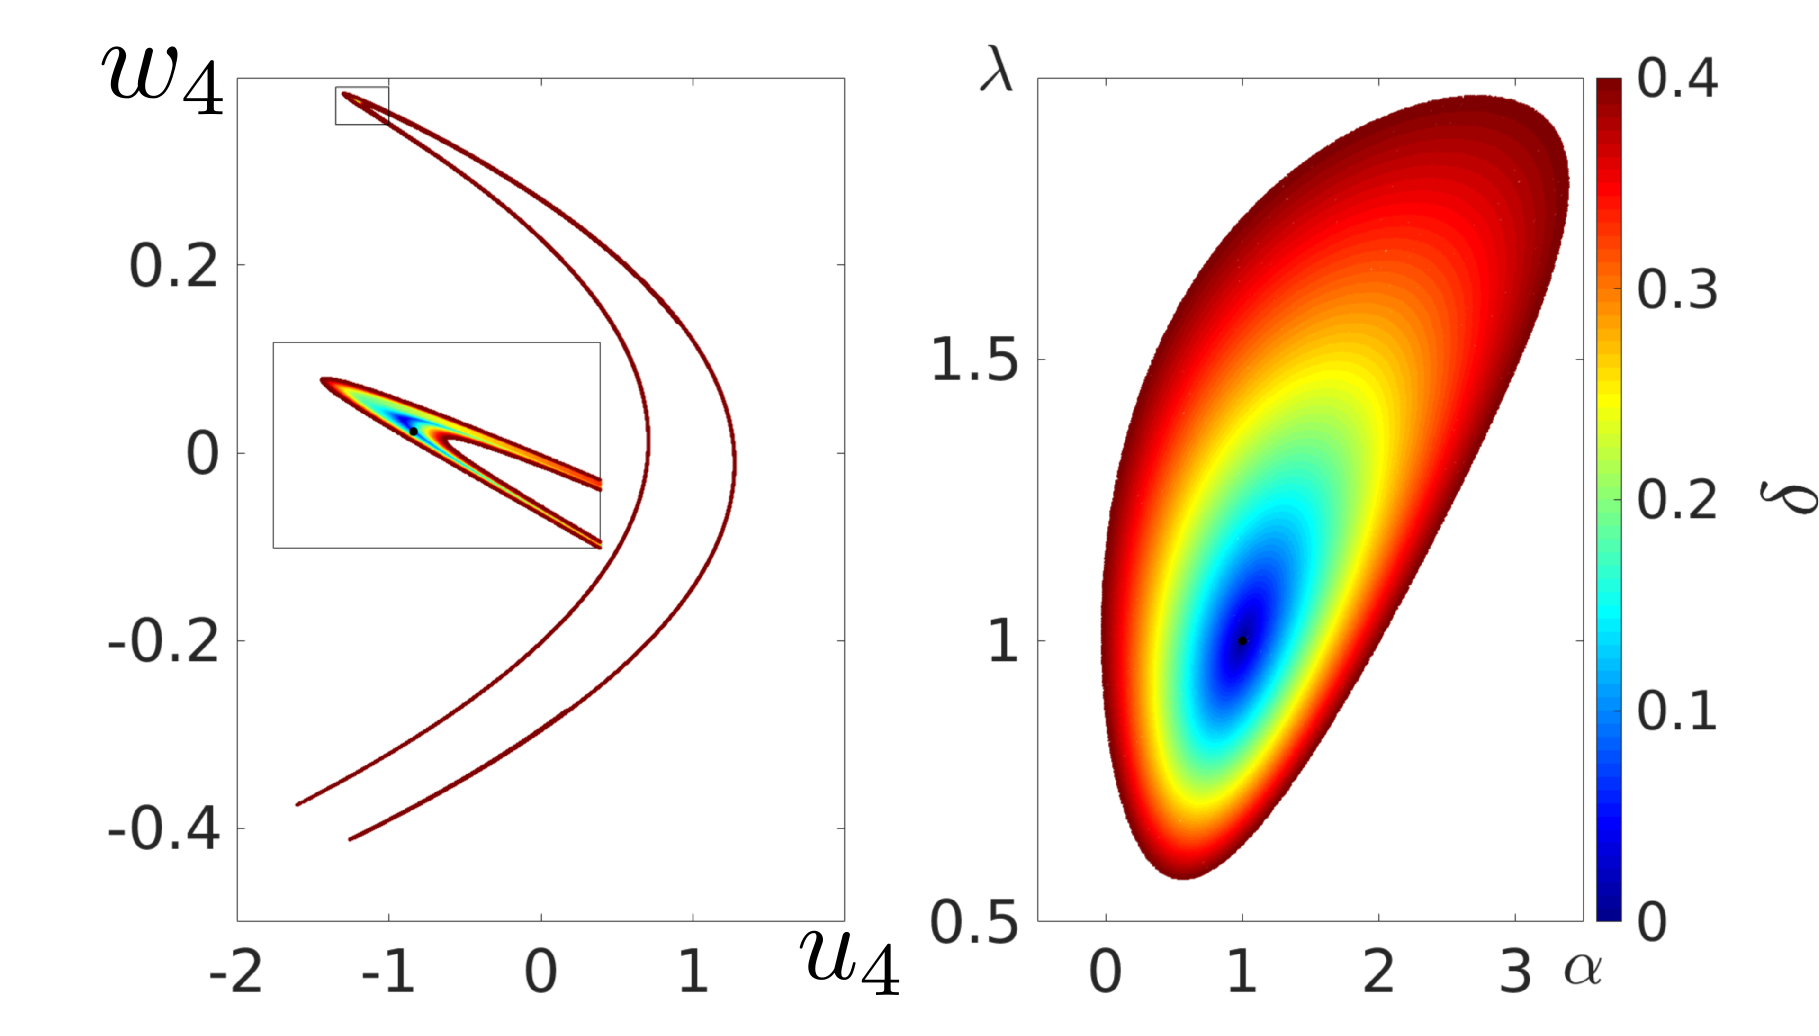
\includegraphics[width=\textwidth]{p2-p1-delta-l-a-delta}
  \caption[H\'{e}non map transformed parameters and original
  parameters in nonlinear singularly perturbed system]{Parameter space colored by $\delta$; all points satisfy $\delta<0.4$. H\'{e}non map transformed parameters $w_4$ and $u_4$ (left), and original parameters $\alpha$ and $\lambda$ (right). Here, we used the classical values  $(\gamma,\zeta) = (1.4,0.3)$ for the H\'{e}non map. The central point at $\delta=0$ corresponds to $(\lambda^*, a^*) = (1, 1)$.
    % $\mathbf{p}^* = (0.7956, 1.8)$
    \label{fig:henon} }
\end{figure*}

\subsection{Unraveling sloppiness} \label{sec:rr} The previous example
demonstrated how a model can be re-parameterized to become sloppy.  Of
much greater practical interest is the inverse procedure, through
which sloppy parameter combinations are identified and factored out.
We work in the concrete setting of the three-species, fully tractable
reaction system
% 
\begin{align}
  A
  \xrightleftharpoons[k_{-1}]{k_1}
  B
  \xrightarrow[]{k_2}
  C .
  \label{mech:abc}
\end{align}

% 
Under mass action kinetics, the concentration of the end product is
given by the analytical expression
% 
\begin{align}
  C(t|\mathbf{p})
  =
  A_0
  \left(
  \frac{k_1 k_2}{\alpha \beta}
  +
  \frac{k_1 k_2}{\alpha(\alpha - \beta)}
  e^{-\alpha t}
  -
  \frac{k_1 k_2}{\beta(\alpha - \beta)}
  e^{-\beta t}
  \right) ,
  \label{eq:cfull}
\end{align}
% 
where $(A_0,B_0,C_0)$ are the fixed constituent concentrations at time
zero and $\alpha,\beta$ depend on $\mathbf{p}=(k_{-1},k_1,k_2)$; see
the SI for the derivation.  In the parameter regime
$k_1 k_2 \ll (k_1 + k_{-1} + k_2)^2$, \eqref{eq:cfull} is well
approximated by
% 
\begin{align}
  C_\mathrm{eff}(t|\mathbf{p})
  =
  A_0
  \left(
  1 - e^{-k_\mathrm{eff} t}
  \right) ,
  \quad
  k_\mathrm{eff}
  =
  \frac{k_1 k_2}{k_{-1} + k_1 + k_2} .
  \label{ABC-QSSA}
\end{align}
% 
Note that this approximate solution extends to a larger parameter
range the quasi-steady state approximation (QSSA)
$C_\mathrm{QSSA}(t|\mathbf{p}) = A_0 (1 - e^{-k_\mathrm{QSSA} t})$,
valid for $k_1 \ll k_{-1} + k_2$ with
$k_\mathrm{QSSA}=k_1 k_2/(k_{-1} + k_2)$.  Plainly, this approximate
solution represents an effective reduction of parameter space down to
the single parameter $k_\mathrm{eff}$, the levels sets of which
foliate parameter space as in Fig.~\ref{fig:dmitri}.

To verify that $C(t)$ remains roughly constant on these level sets, we
choose reference parameter settings $\mathbf{p}^*$ in the regime
identified above, fix sampling times $t_1,\ldots,t_N$, set the model
response to
$\mathbf{f}(\mathbf{p})=( C(t_1|\mathbf{p}) , \ldots ,
C(t_N|\mathbf{p}) )$, sample log-parameter space uniformly, and record
the squared Euclidean distance
$\delta(\mathbf{p}) = \| \mathbf{f}(\mathbf{p}) - \mathbf{f}^* \|^2$
for each sampled $\mathbf{p}$.  The result is shown in
Fig.~\ref{fig:abc-keff}, where we have only retained parameter
combinations with $\delta(\mathbf{p}) < 10^{-6}$.  As expected, the
level sets of constant $\delta$ align with those of the effective
parameter, so this automated sampling process effectively reveals
sheets of the foliation in Fig.~\ref{fig:dmitri} without recourse to
an analytic expression for $k_\mathrm{eff}$.

\begin{figure}[ht!]
  \centering
  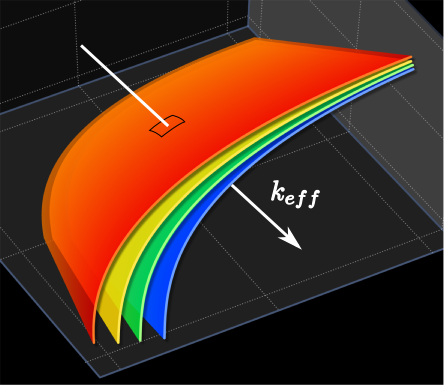
\includegraphics[width=0.5\textwidth]{keff-illustration}
  \caption[Illustration of level sets of the effective parameter in a
  model of chemical kinetics]{Illustration of level sets of $k_{eff}$
    in parameter space. \label{fig:dmitri} }
\end{figure}

By coloring these points by $\delta(\mathbf{p})$, we can observe the
direction in parameter space along which $\delta(\mathbf{p})$ varies,
or, equivalently, along which model response changes. This naturally
corresponds to the directions orthogonal to the sloppy manifold, but
more importantly, the right figure shows that it also matches the
direction in which $k_{eff}$ changes. This follows from our previous
result that, in this region of parameter space,
$\delta(\mathbf{p}) \approx \delta(k_{eff})$.  Note that, in fact,
even when our parameters do not obey the inequalities we presented
above, we will still be faced with sloppy parameters. This arises from
the fact that regardless which parameters are used, $C(t)$ is always a
function of just two overall parameters, giving rise to a
one-dimensional sloppy manifold. Further details on this
non-identifiable parameter are given in Appendix~\ref{ap:abc}.

\begin{figure}[ht!]
  \centering
  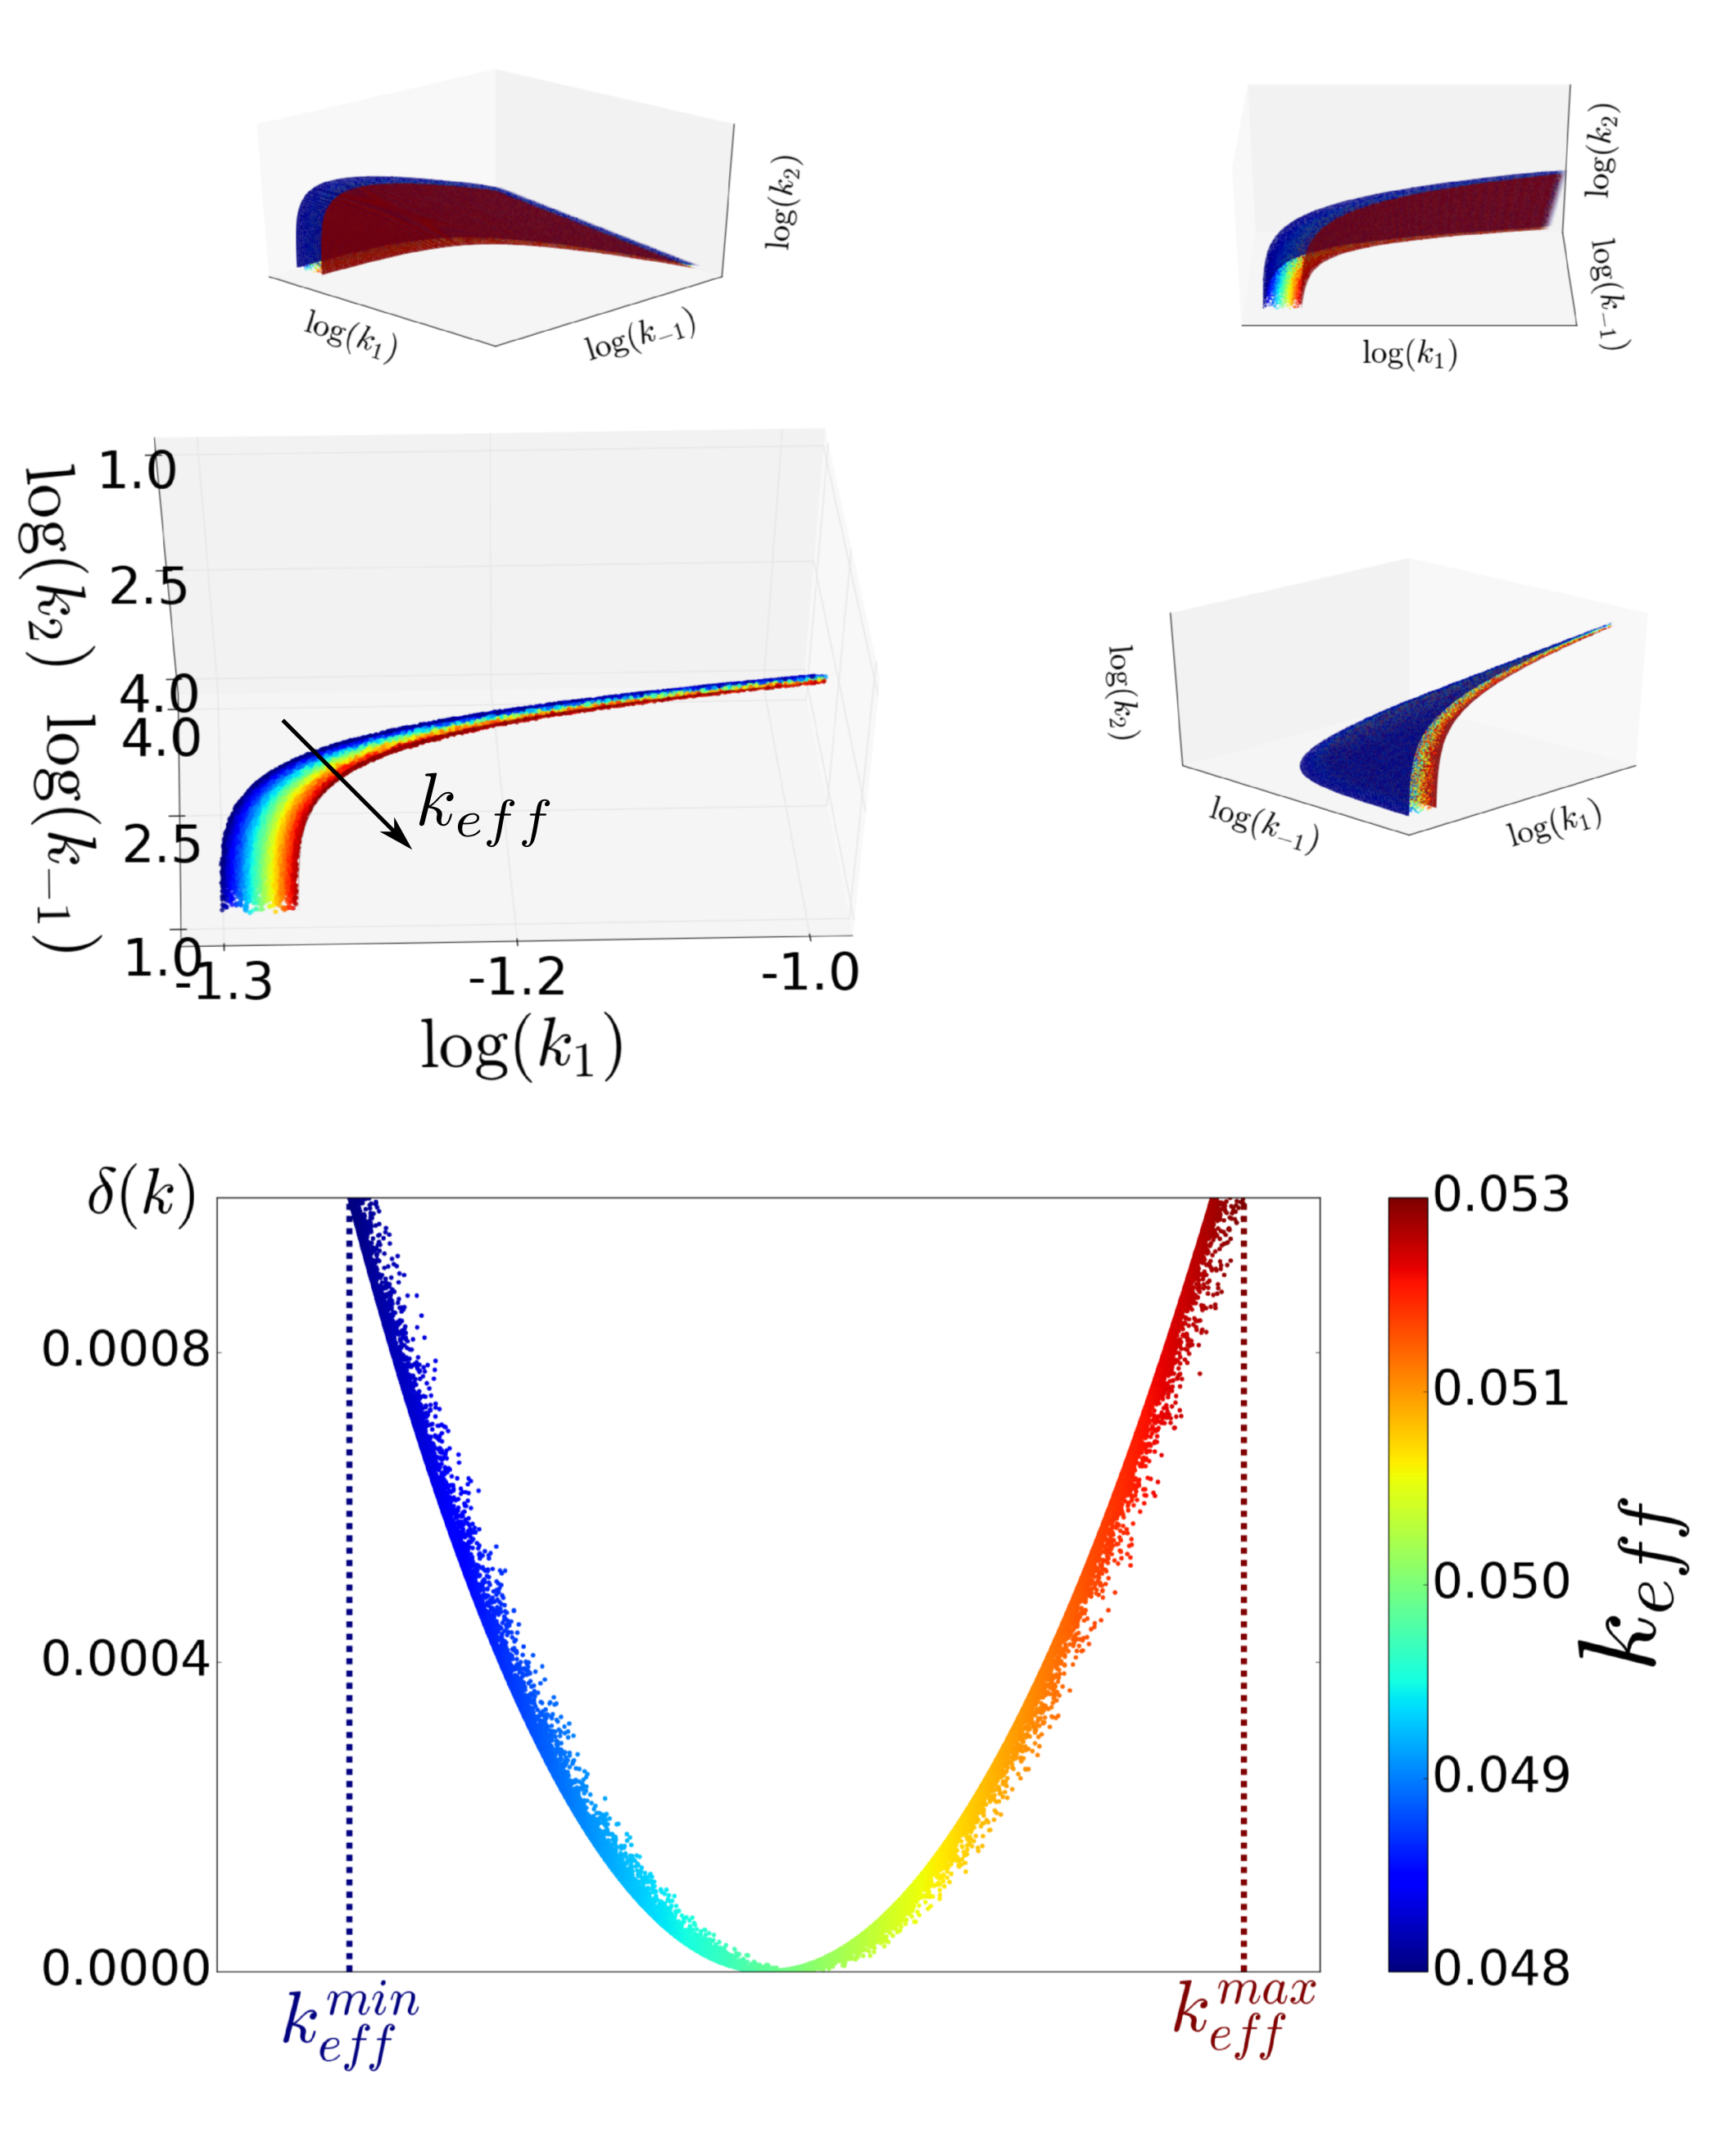
\includegraphics[width=0.5\textwidth]{keffs-delta-keff-vertical}
  \caption[Quantitative three-dimensional views of level sets of the
  effective parameter in a model of chemical kinetics]{(top) Region of
    parameter space lying within large value of $\delta = 10^{-3}$,
    colored by $k_{eff}$. Smaller rotations show three-dimensional
    structure. (bottom) Plot of $\delta$ vs $k_{eff}$ over the dataset
    showing that $\delta(k_1, k_{-1}, k_2) = \delta(k_{eff})$ as
    expected from the reduced reaction kinetics. \label{fig:abc-keff}
  }
\end{figure}

\subsection{Algorithmic parameterization of sloppiness}
Typical detailed models involve tens of parameters, making a visual
analysis of sloppiness like that presented above impossible.
Therefore, we turn to the main contribution of this paper: an
automated method to uncover parameter sloppiness in high dimensional
datasets.  Its foundation is the manifold learning technique Diffusion
Maps (DMAPS) which, broadly speaking, coordinatizes the
lower-dimensional, smooth, curved manifold best containing a data set
embedded in some high-dimensional data space.  As we will see in
detail, combining DMAPS with the parameter sampling described above
leads to the identification of sloppy neutral sets and, through them,
of effective system parameters.

\subsection{Diffusion Maps}

We now present the DMAPS algorithm; further details can be found in
\cite{}. We begin with a set of $N$ points in $\mathbb{R}^p$,
$\{\mathbf{p}_i\}_{i=1}^N$, here a set of parameter combinations. Next
we calculate a kernel matrix whose entries are given by

\begin{align}
  W_{ij} = \exp\bigg(-\frac{\| \mathbf{p}_i - \mathbf{p}_j \|^2}{\epsilon^2}\bigg)
  \label{eq:dmaps-w}
\end{align}

where $\epsilon$ is a tunable parameter that defines the neighborhood
of each point (note that pairs of points for which
$\|\mathbf{p}_i - \mathbf{p}_j\| > \epsilon$ lead to
$W_{ij} \approx 0$ while if
$\|\mathbf{p}_i - \mathbf{p}_j\| < \epsilon$ we have
$W_{ij} \approx 1$). We normalize the entries of this matrix to create
a new matrix $A$ in which

\begin{align}
  A_{ij} = \frac{W_{ij}}{d_i} = \frac{W_{ij}}{\sum_j W_{ij}}
  \label{eq:dmaps-a}
\end{align}

As $0 < A_{ij} < 1$ and $\sum_i A_{ij} = 1$, $A$ is a Markov matrix
and we can interpret $A_{ij}$ as the probability of hopping from point
$\mathbf{p}_i$ to $\mathbf{p}_j$ in parameter space. Intuitively, as
the distance between points decreases, this probability increases. It
can be shown that this matrix $A$ approximates the Laplace-Beltrami
operator on the manifold, and that under certain conditions, its
eigenvectors and eigenvalues converge to the eigenfunctions and
eigenvectors of the Laplace-Beltrami operator with homogeneous Neumann
boundary conditions. It is these eigenvectors that provide the desired
parameterization of the manifold.

The final step in the algorithm is then to compute a partial
eigendecomposition of $A$ to find a set of $k$ eigenvalues and
eigenvectors $\{\phi_i, \lambda_i\}_{i=0}^k$. The diffusion map is
finally given by the function
$\Phi_t : \mathbb{R}^p \rightarrow \mathbb{R}^k$

\begin{align}
  \Phi_t(x_i) = \begin{bmatrix} \lambda_1^t \phi_1(i) \\ \lambda_2^t
    \phi_2(i) \\ \vdots \\ \lambda_k^t \phi_k(i) \end{bmatrix}
\end{align}

where $\phi(i)$ represents the $i^{th}$ component of vector
$\phi$. The idea is that these eigenvectors parameterize the manifold
on which our points lie, and that if we can find this parameterization
for some $k \ll p$ we can describe our dataset using this alternative
parameterization to achieve dimensionality reduction.

When we apply this method to our dataset for which $\delta < 10^{-6}$,
we find that the eigenvectors $\phi_1$ and $\phi_2$ provide the
desired coordinates on the nonlinear surface. This is illustrated in
Fig. (\ref{fig:abc-dmaps}) in which the surface is colored by $\phi_1$
and $\phi_2$ values. As these eigenvectors map out independent
directions on the data, we may use them as an alternative coordinate
system for our points. In effect, DMAPS has given us a
parameterization of the sloppiness in our model.

\begin{figure*}
  \centering
  \begin{subfigure}[t]{0.45\linewidth}
    \centering
    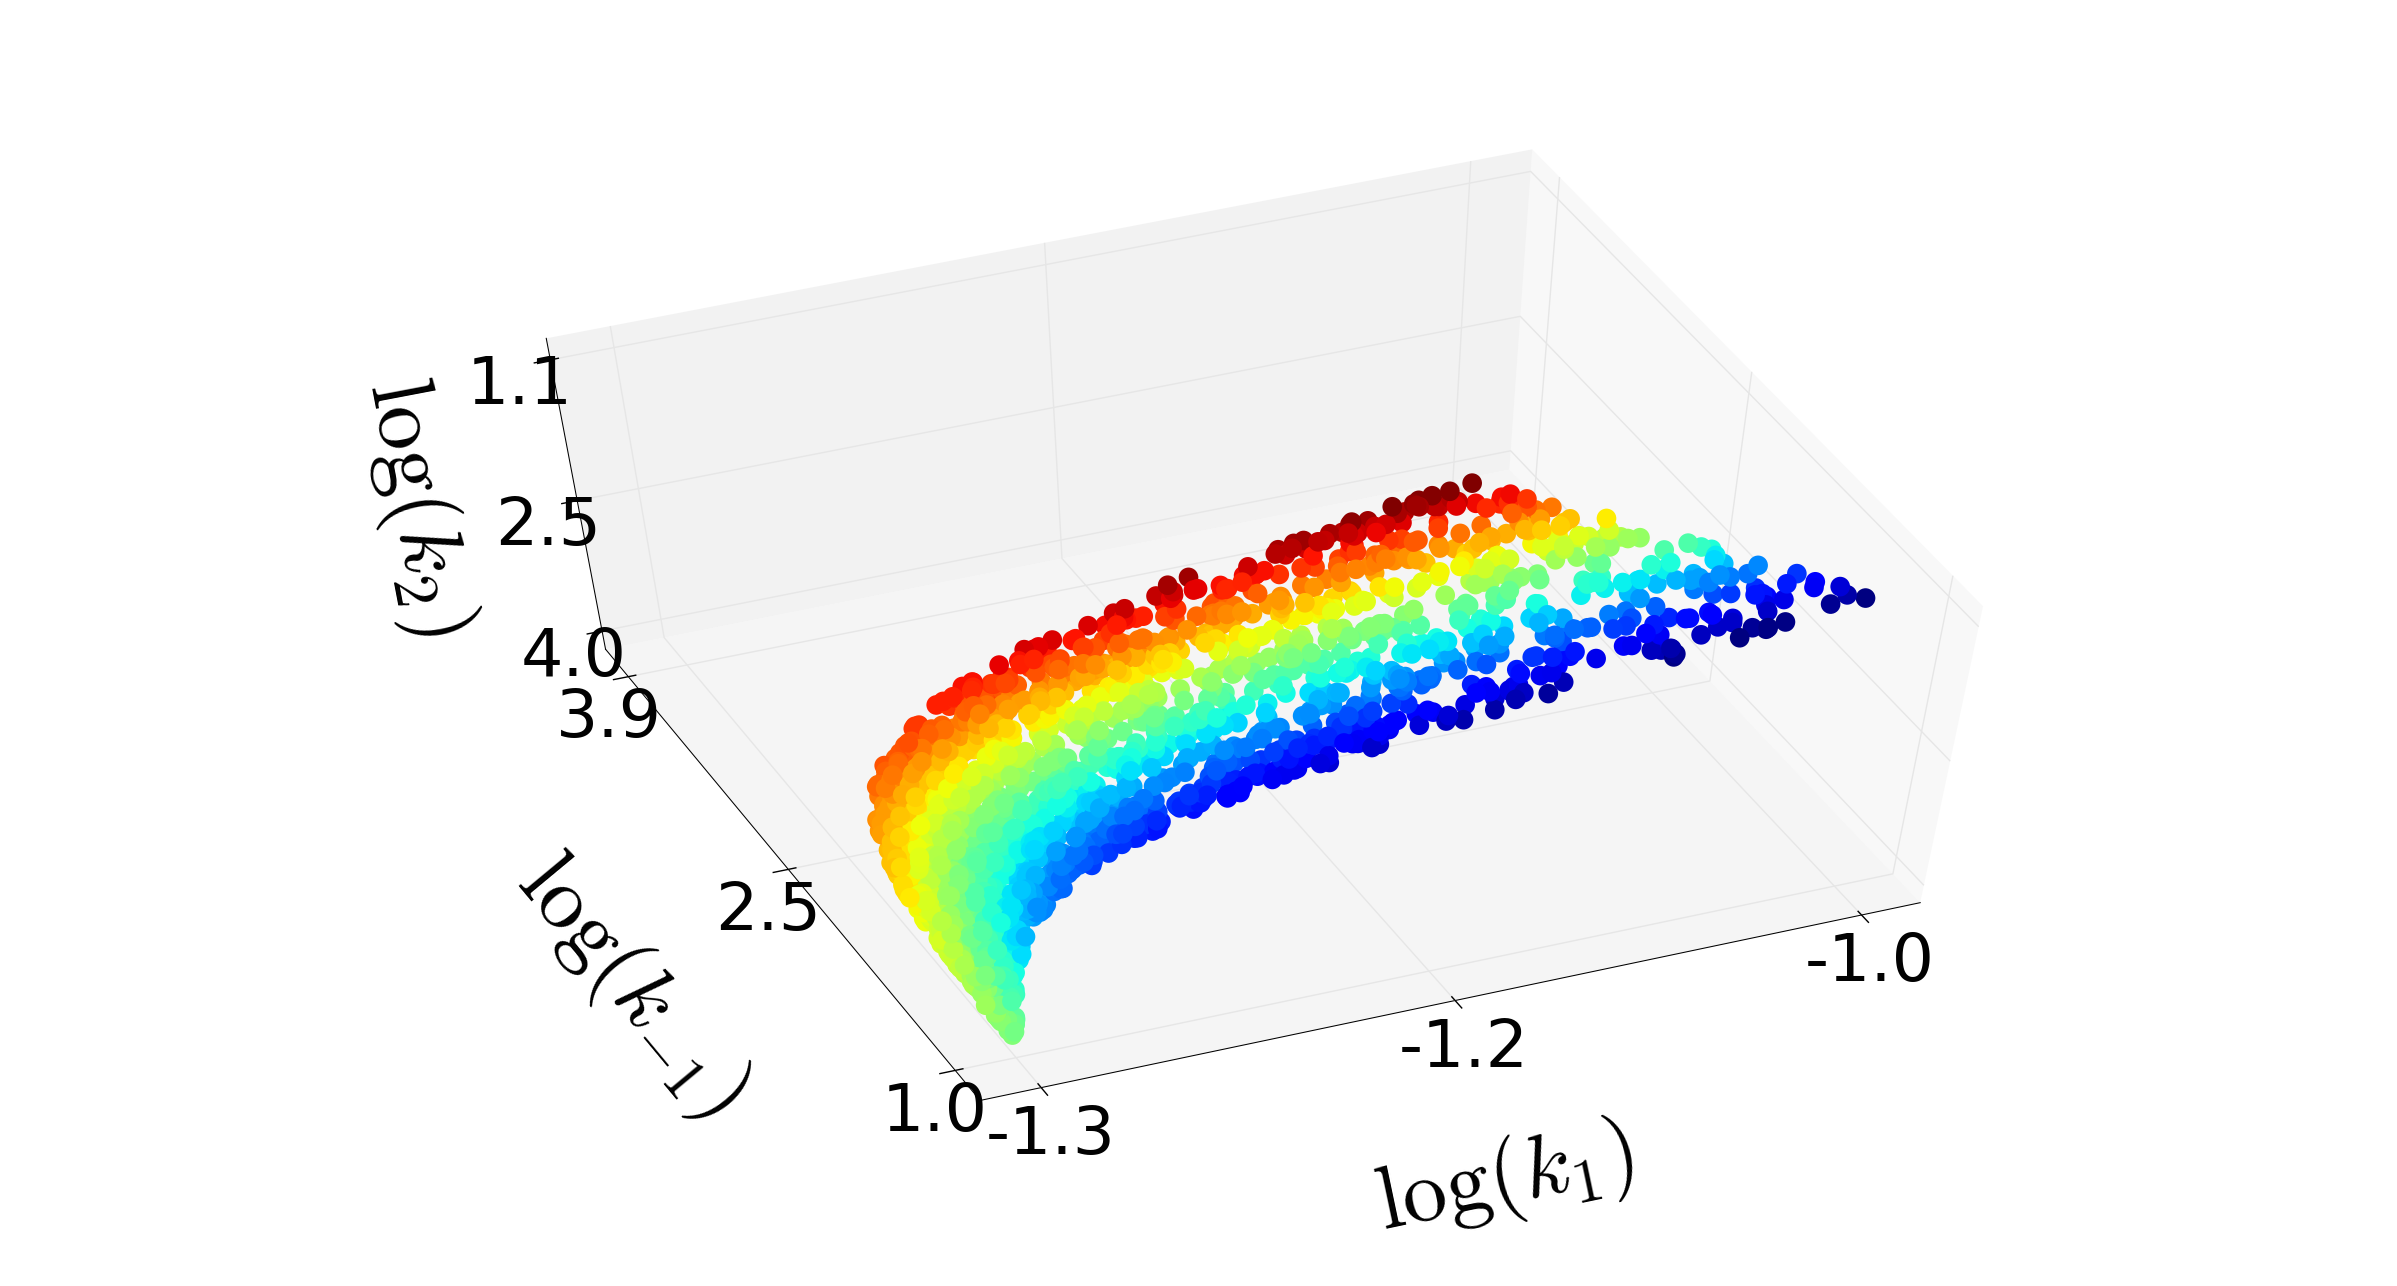
\includegraphics[height=2in]{k1-kinv-k2-phi1}
    % \subcaption{ \label{ks-p-phi1} }%
  \end{subfigure}
  \hspace{0.5cm}
  \begin{subfigure}[t]{0.45\linewidth}
    \centering
    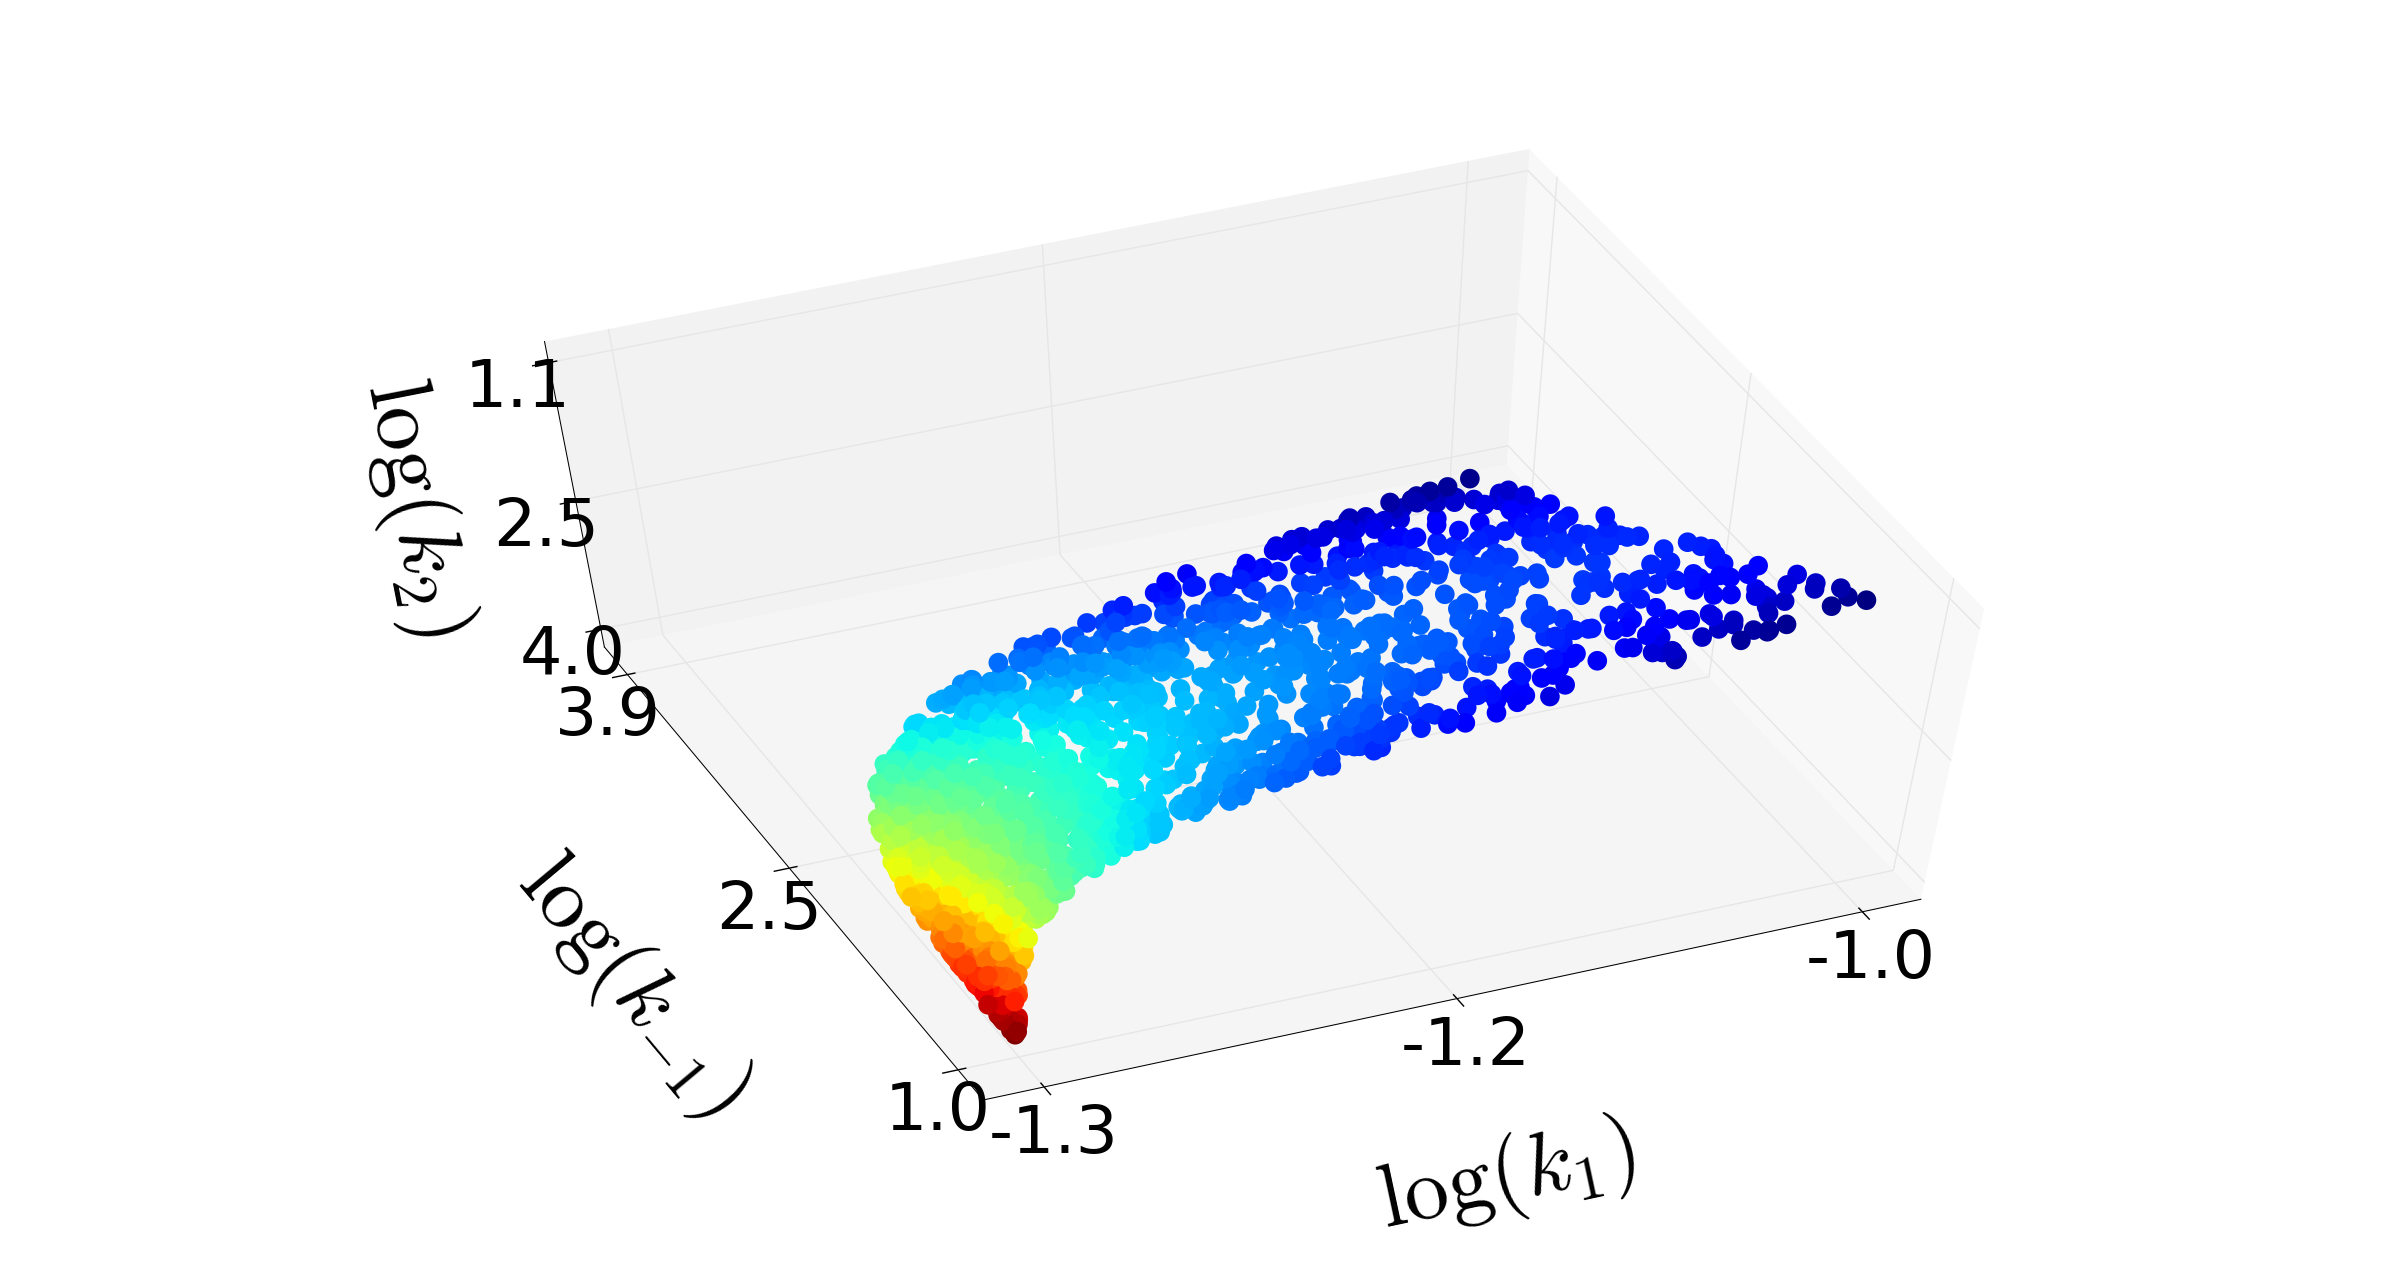
\includegraphics[height=2in]{k1-kinv-k2-phi2}
    % \subcaption{ \label{ks-p-phi2} }%
  \end{subfigure}
  \caption[Parameter space of kinetics model colored by DMAPS
  output]{Parameter space colored by $\phi_1$ (left) and $\phi_2$
    (right), which uncovers one of the directions along this nonlinear
    sloppy manifold. \label{fig:abc-dmaps} }
\end{figure*}

If we apply this same technique to the dataset we previously discussed
in Fig.~\ref{fig:henon}, we are met with less success. Although the
nonlinearities do not pose a problem for DMAPS, the disparate
lengthscales do. The model here is two-dimensional as both $a$ and
$\lambda$ are significant parameters; however, applying DMAPS to
parameter space suggests a one-dimensional system. This is shown in
Fig.~\ref{fig:henon-paramspace-dmaps}.

\begin{figure*}
  \centering
  \begin{subfigure}[t]{0.45\linewidth}
    \centering
    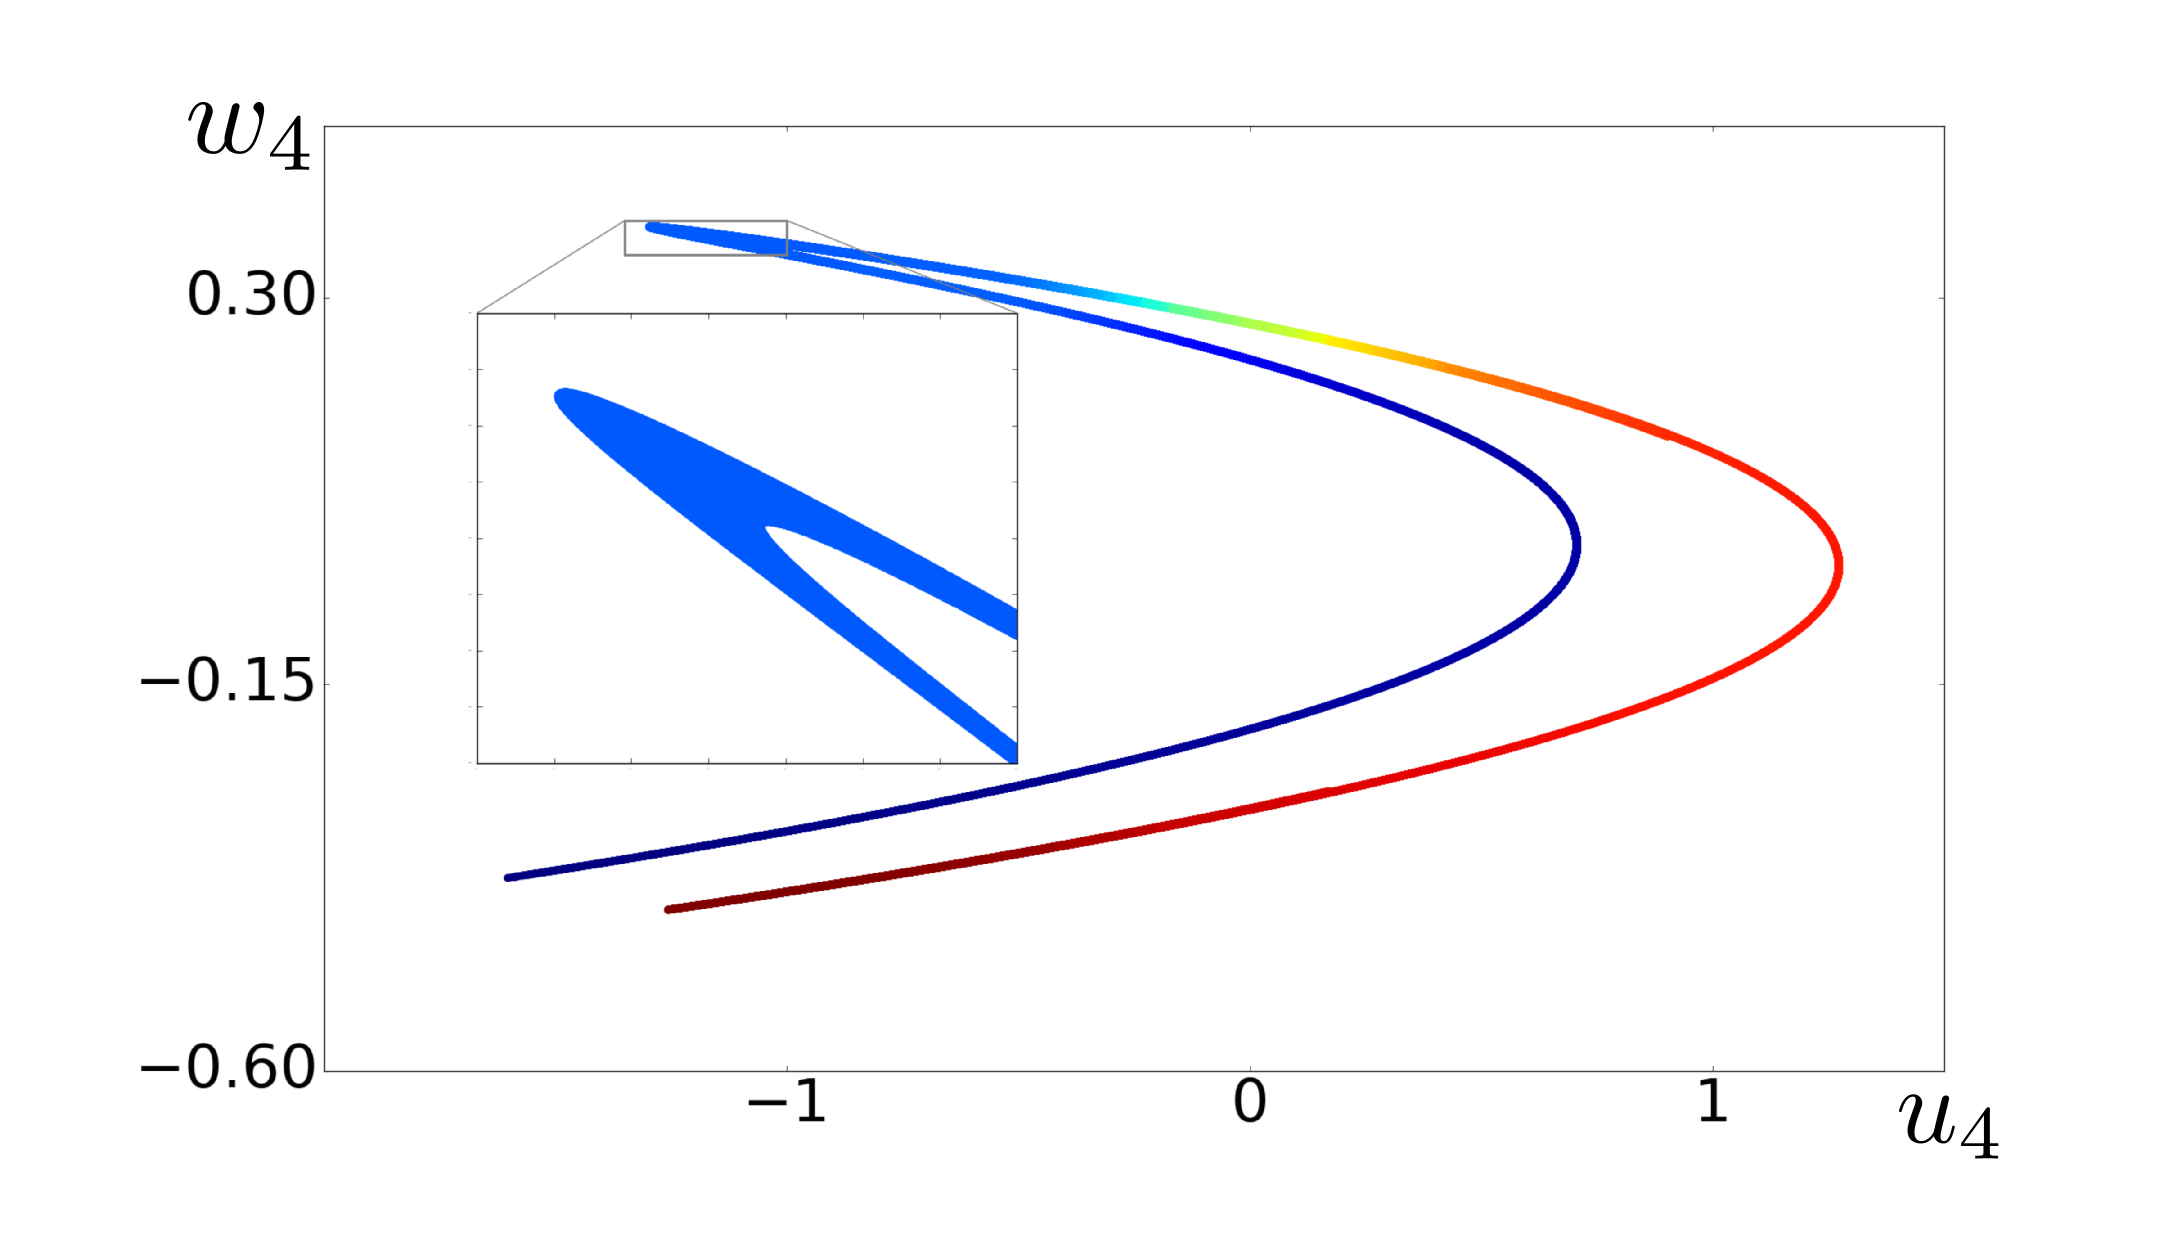
\includegraphics[width=1.0\linewidth]{y4-x4-phi1-paramspace-dmaps}
    \subcaption{Coloring of $(u_4, w_4)$ samples by $\phi_1$, where
      $\phi_1$ is the result of DMAPS applied only to parameter
      space. While the model manifold remains two-dimensional, the
      nonlinear transformation of parameter space affected by the
      H\'{e}non map causes the system to appear one-dimensional.}
  \end{subfigure}
  \hspace{0.5cm}
  \begin{subfigure}[t]{0.45\linewidth}
    \centering
    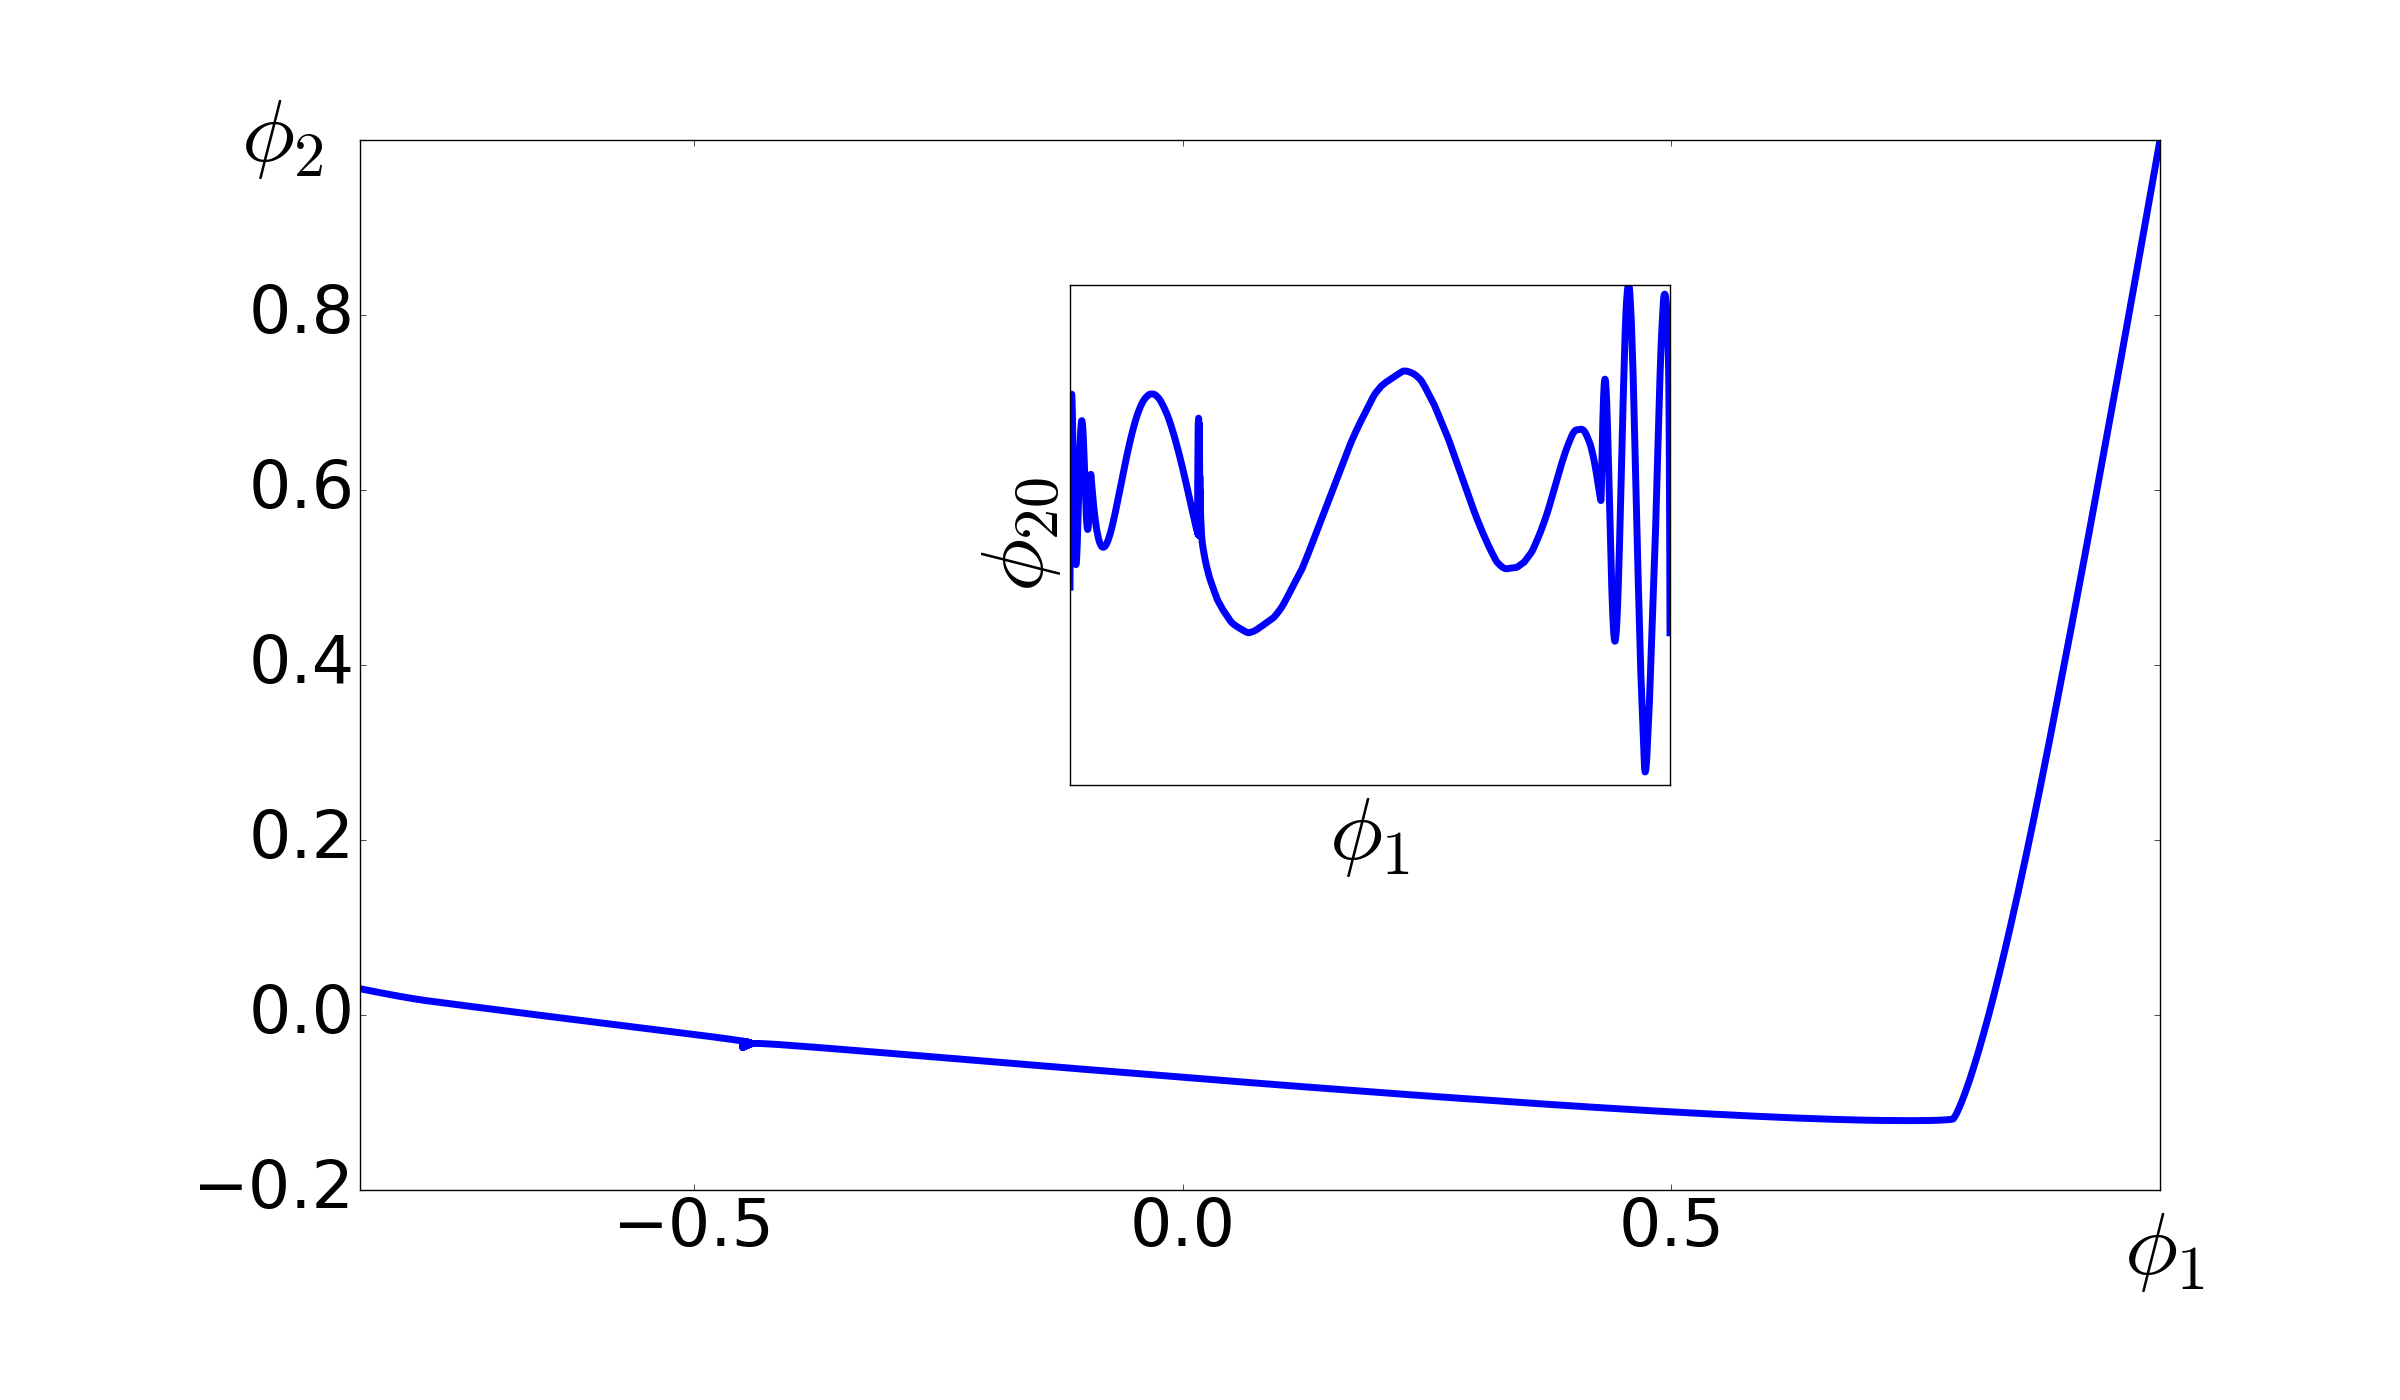
\includegraphics[width=1.0\linewidth]{phi2-phi1-paramspace-dmaps}
    \subcaption{Plot of DMAP embedding in $\phi_1$ and $\phi_2$ (main
      figure), and in $\phi_1$ and $\phi_{20}$ (inset). As $\phi_1$ is
      the only independent DMAP eigenvector, we incorrectly identify
      our system as one-dimensional. This shows the importance of
      including model manifold information when using DMAPS to reduce
      the dimensionality of the parameter set.}
  \end{subfigure}
  \caption[Parameter space of singularly perturbed system colored by
  DMAPS]
  {Result of applying DMAPS to transformed parameter space,
    incorrectly identifying the system as
    one-dimensional. \label{fig:henon-paramspace-dmaps} }
\end{figure*}


Another issue arising from this basic application of DMAPS stems from
non-invertible models, in which multiple points in parameter space are
mapped to the same model response.

INSERT

Finally, we are typically more interested in the directions along
which model predictions vary than those along which predictions are
constant: the influential directions in parameter space as opposed to
the sloppy directions. As we will see, by employing a modified version
of DMAPS we can recover such important directions and avoid the sorts
of misclassifications shown in Fig.~\ref{fig:henon-paramspace-dmaps}
and Fig.~\ref{fig:noninvertible}.

\subsection{Anisotropic Diffusion Maps}

The key is to modify the kernel in \eqref{eq:dmaps-w} to bias our
random walk along parameter directions in which model predictions
remain constant. This is achieved through the form

\begin{align}
  W_{ij} = \exp\bigg(-\frac{1}{\epsilon^2} \big(\| \mathbf{p}_i - \mathbf{p}_j
  \|^2 + \frac{\|\mathbf{f}(\mathbf{p}_i) - \mathbf{f}(\mathbf{p}_j) \|^2}{\lambda^2} \big) \bigg)
  \label{eq:dmaps-w-mod}
\end{align}

By adding the
$\|\mathbf{f}(\mathbf{p}_i) - \mathbf{f}(\mathbf{p}_j) \|$ term we
create an anisotropic diffusion on the parameter set that we can bias,
through the parameters $\epsilon$ and $\lambda$, in directions along
which model predictions are constant. We then expect the leading
eigenvectors of the modified diffusion map to parameterize directions
orthogonal to these sloppy surfaces, giving coordinates for the
important parameter space directions.

We apply this method to the dataset shown in Fig.~\ref{fig:abc-keff}
in which all parameter combinations satisfy
$c(\mathbf{p}_i) < 10^{-3}$. The results shown in
Fig.~\ref{fig:abc-datadmaps} reveal that the first eigenvector
$\phi_1$ parameterizes the direction along which $k_{eff}$ changes, as
desired. That is, $\phi_1$ parameterizes the important direction in
this model in that increasing values of $\phi_1$ correspond to
decreasing values of $k_{eff}$. By using the modified kernel in
\eqref{eq:dmaps-w-mod} we have succeeded in uncovering both the
important directions in parameter space from nothing more than a
black-box model evaluator.

\begin{figure}[ht!]
  \centering
  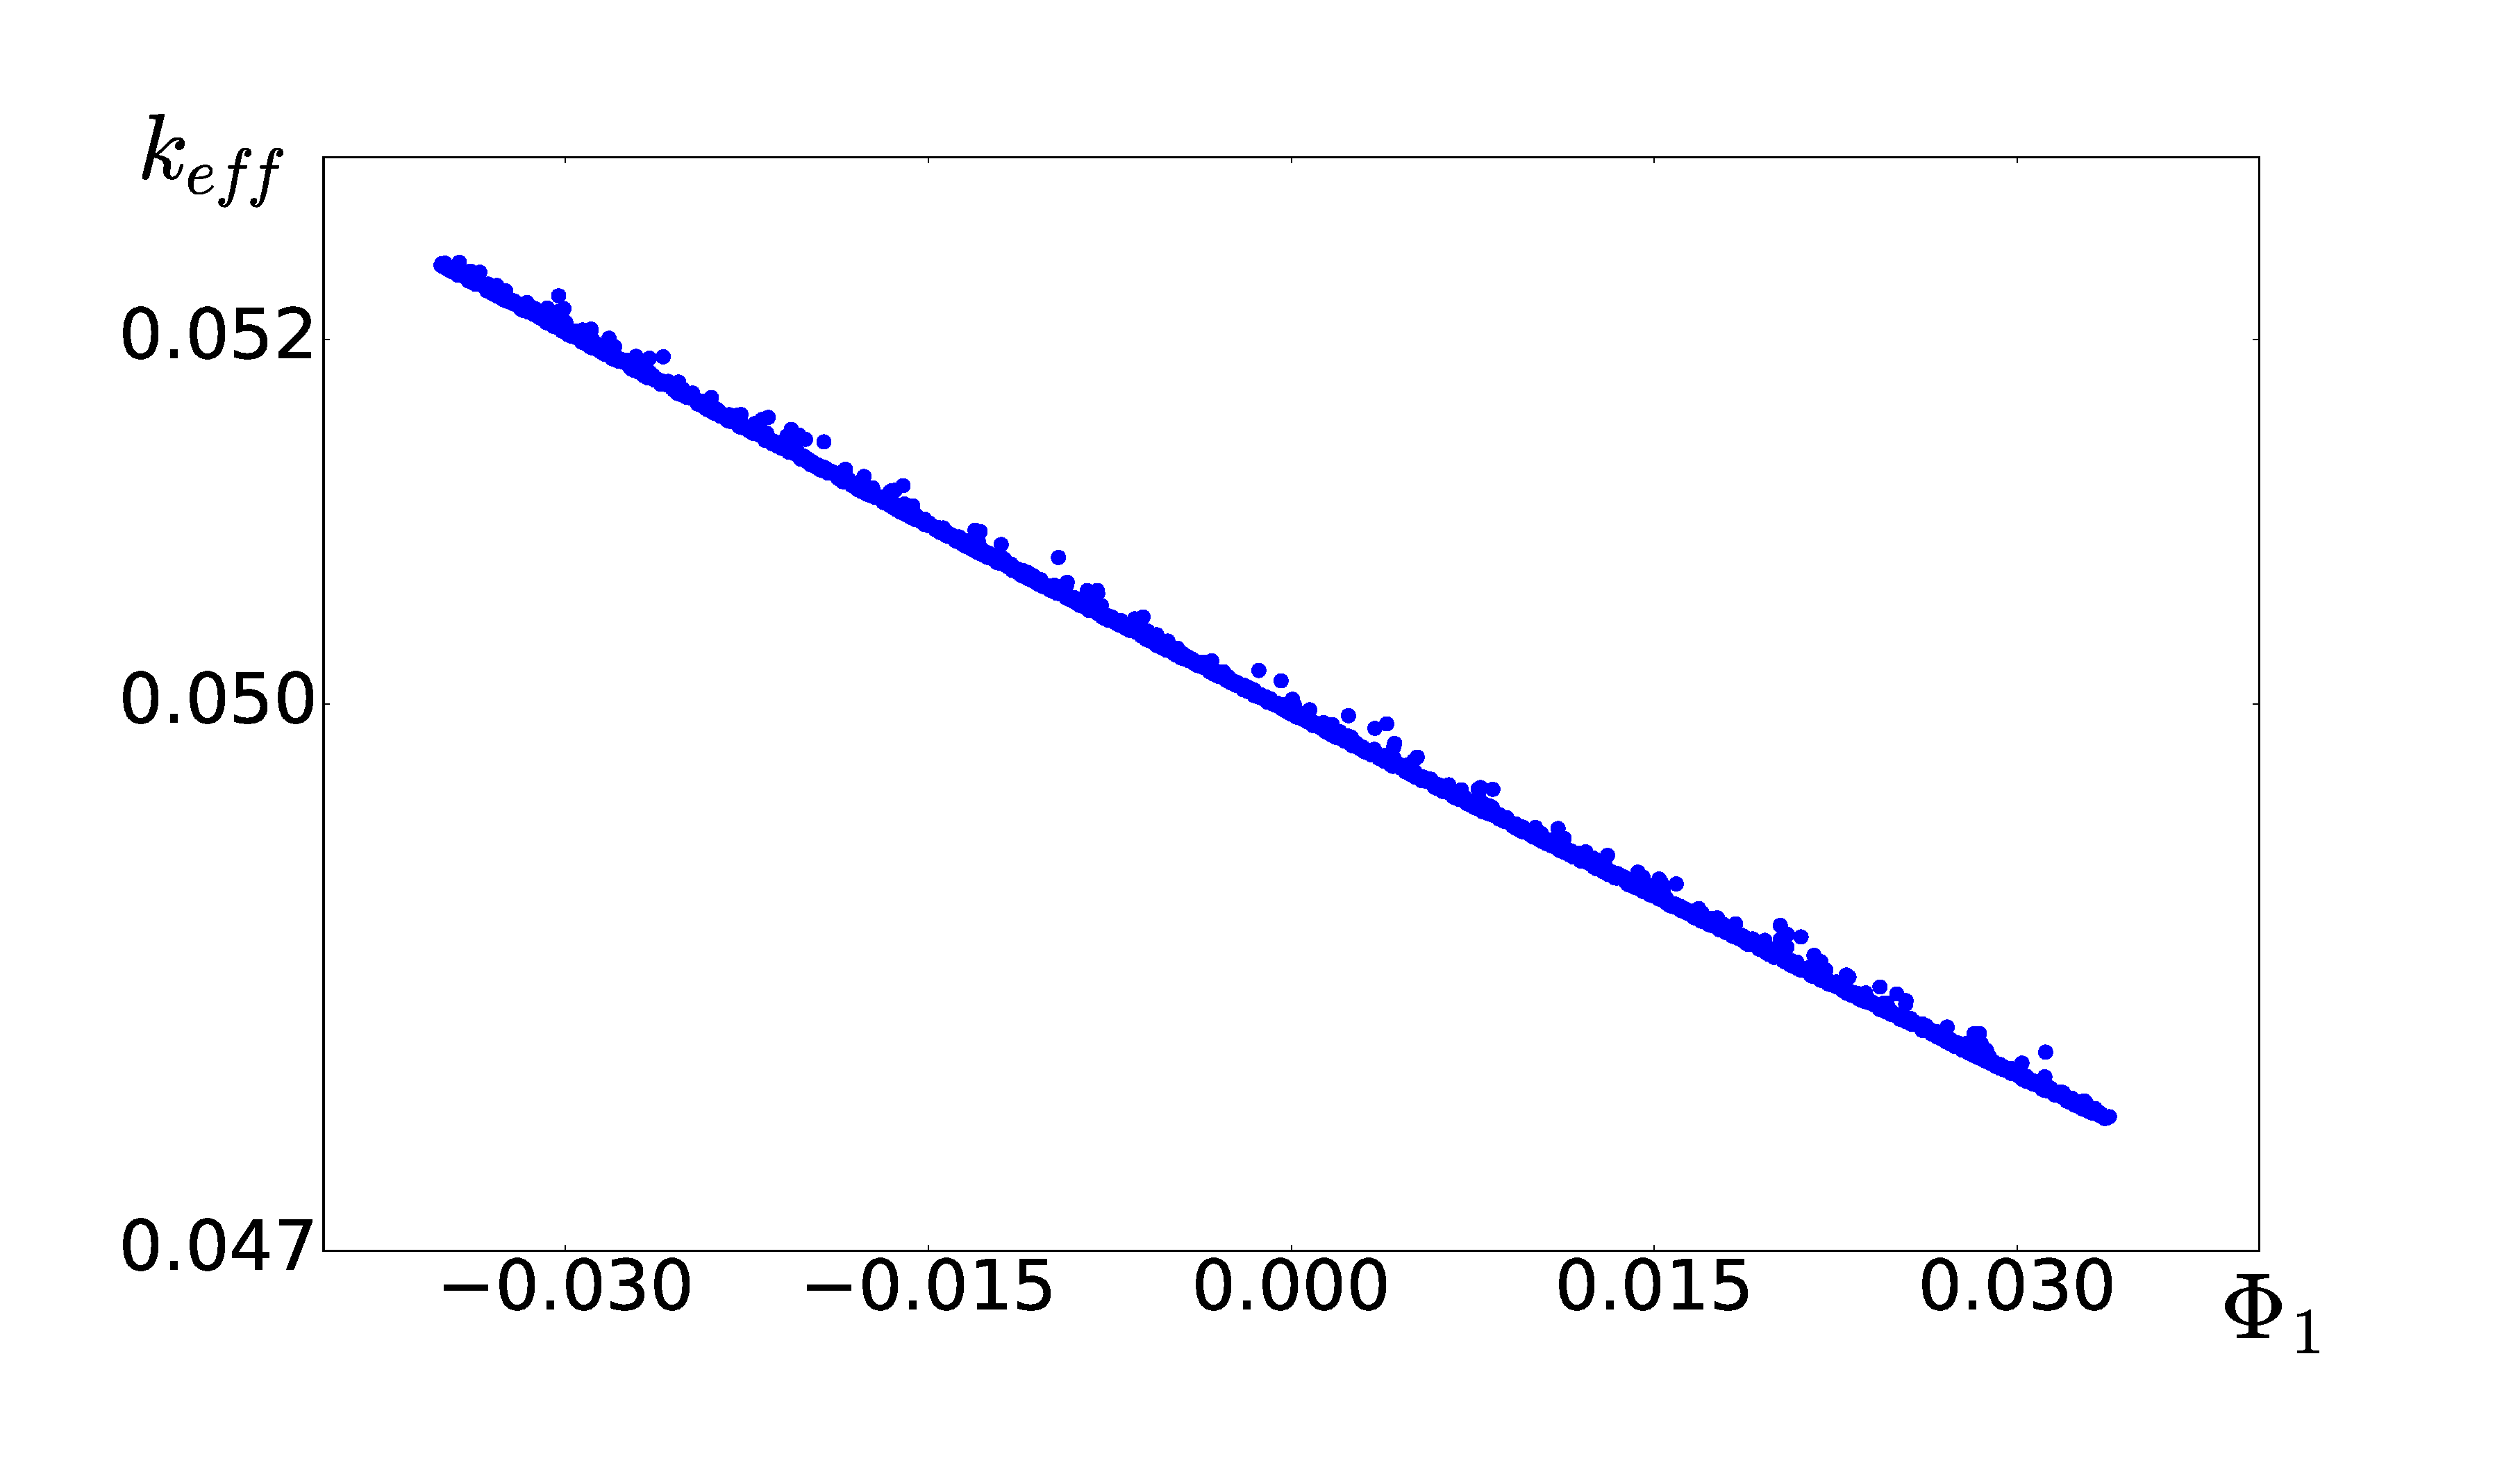
\includegraphics[width=0.5\textwidth, height=2in]{keff-phi1}
  \caption[Plot of effective parameter vs. a DMAPS
  coordinate]{$k_{eff}$ plotted against $\phi_1$ showing that the
    first DMAPS eigenvector parameterizes the significant, nonlinear
    parameter combination hidden in our
    model. \label{fig:abc-datadmaps} }
\end{figure}

\clearpage

To offer another example of this method's utility, we apply our
modified DMAPS to the dataset in Fig.~\ref{fig:henon}. Including
information about the two-dimensional model manifold allows us to
recover the fact that our system is not one-dimensional, even though
our parameter space suggests otherwise. We find a two-dimensional
embedding consistent with the true dimensionality of the system. This
is shown in Fig.~\ref{fig:henon-data-dmaps}.


\begin{figure*}
  \begin{minipage}[c][13cm][t]{.5\textwidth}
    \vspace{2cm} \centering
    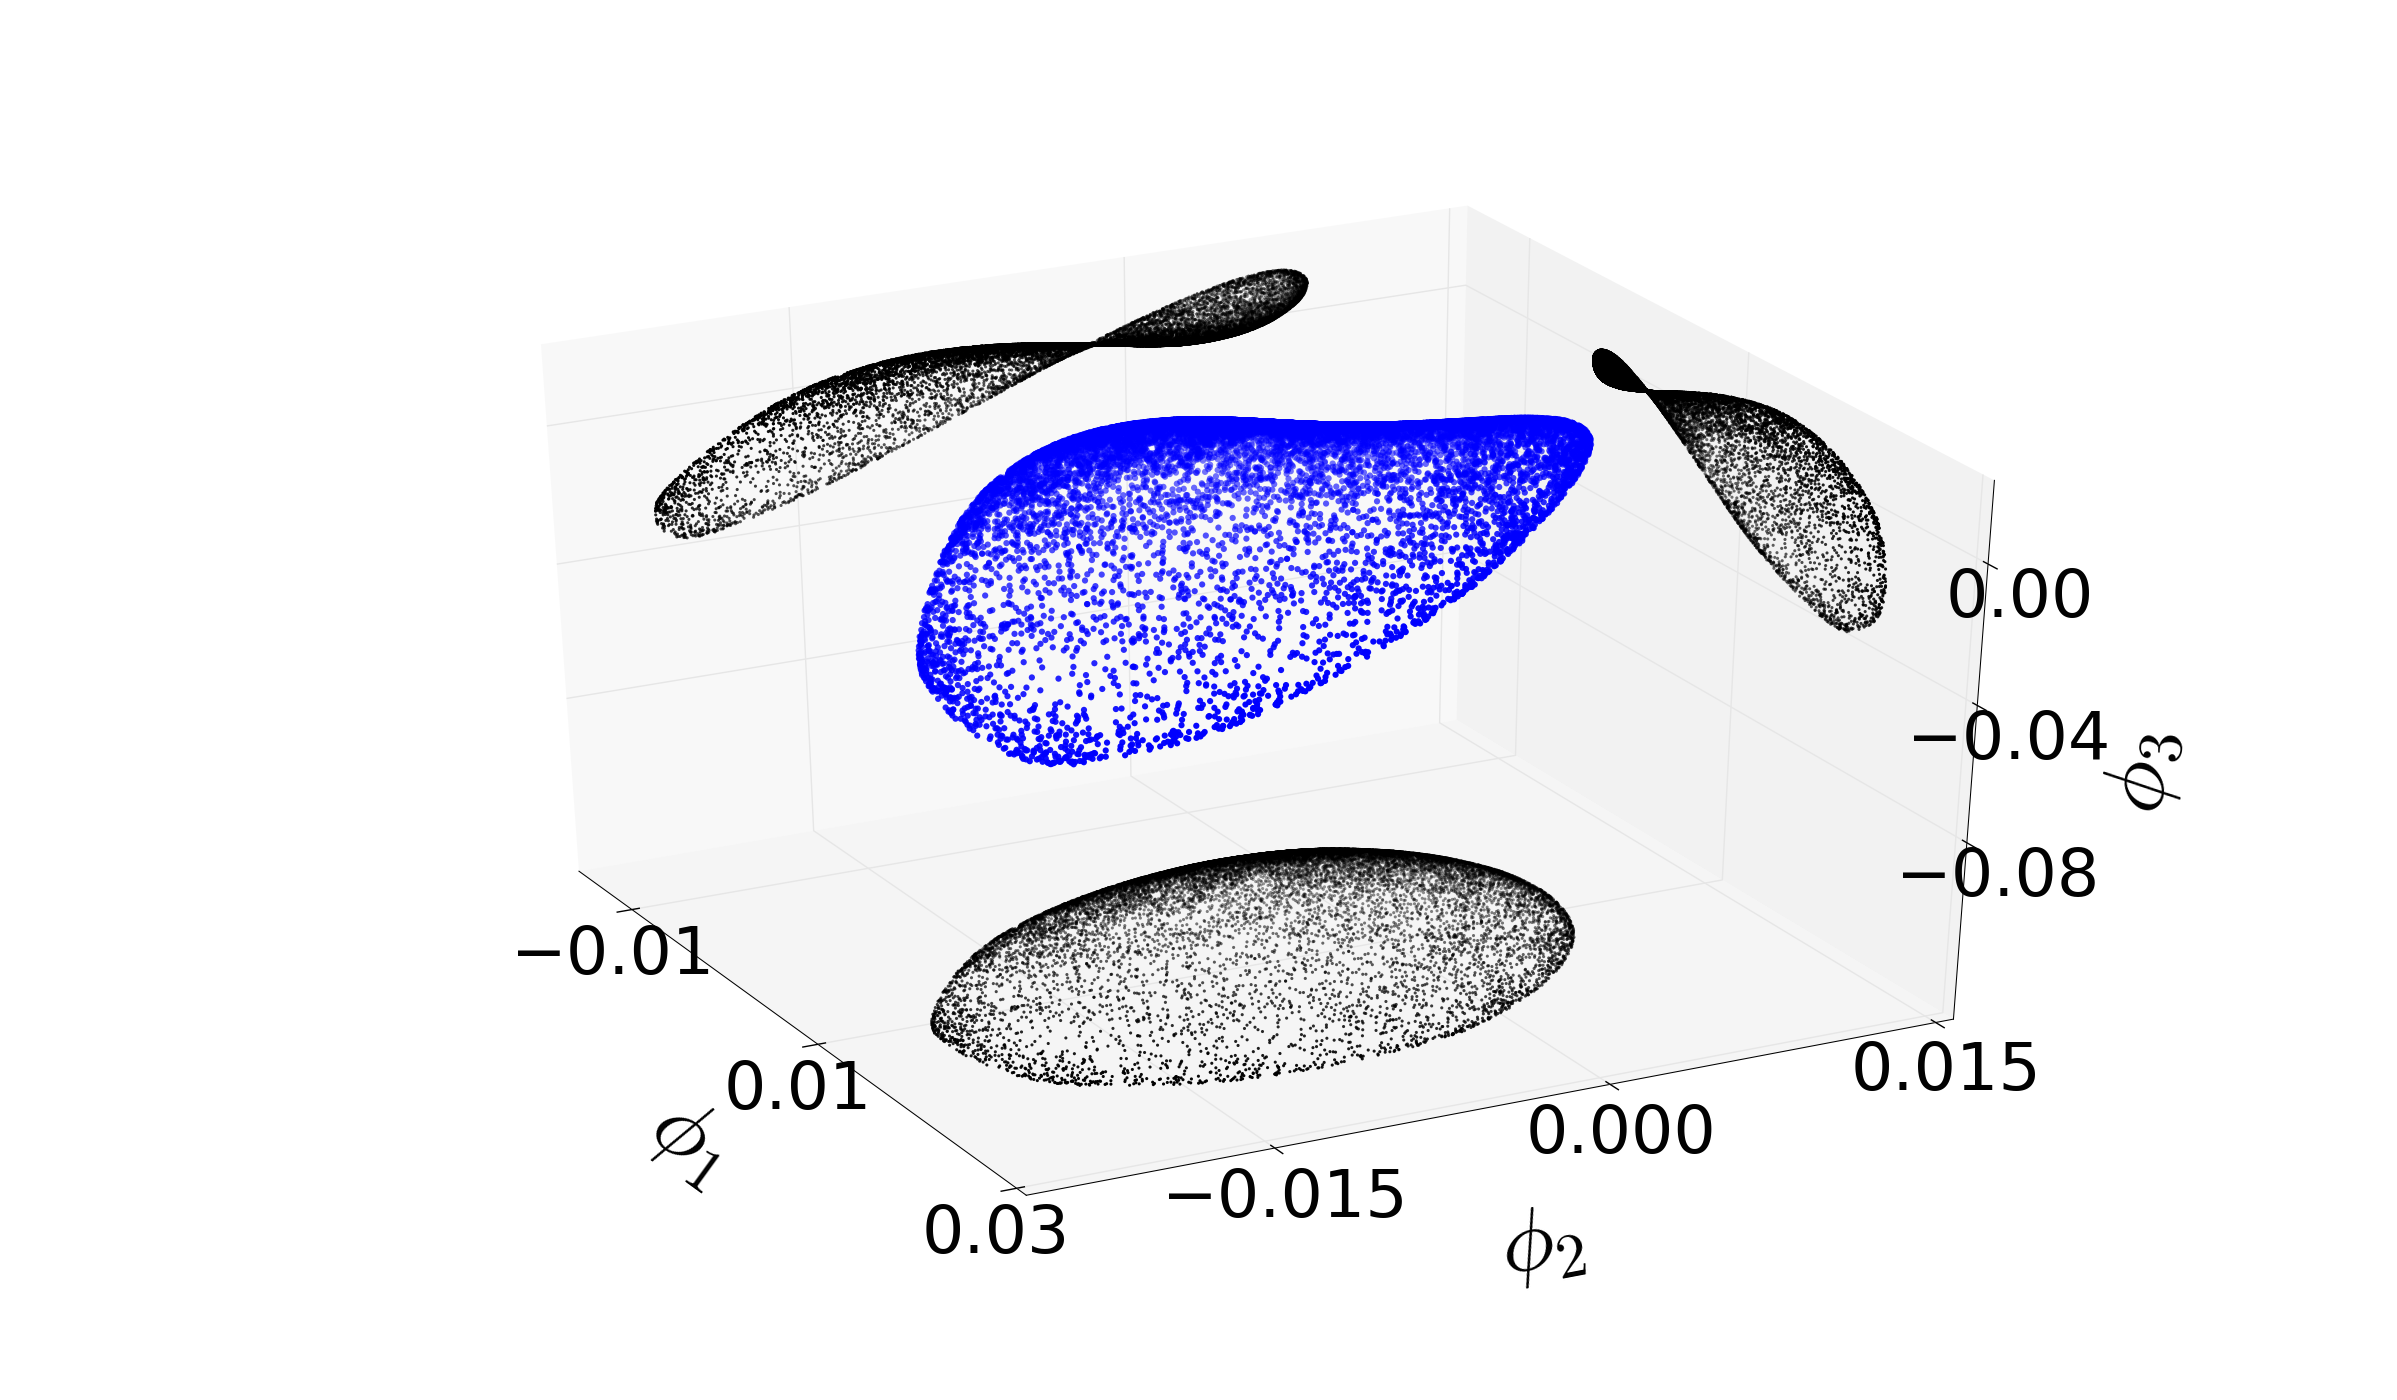
\includegraphics[width=\textwidth]{phi3-phi2-phi1-projections}
    \subcaption{Embedding of dataset in first three eigenvectors,
      suggesting that DMAPS produces a two-dimensional embedding as
      expected.}
    \label{fig:test1}
  \end{minipage}%
  \begin{minipage}[c][13cm][t]{.5\textwidth}
    \vspace{\fill} \centering
    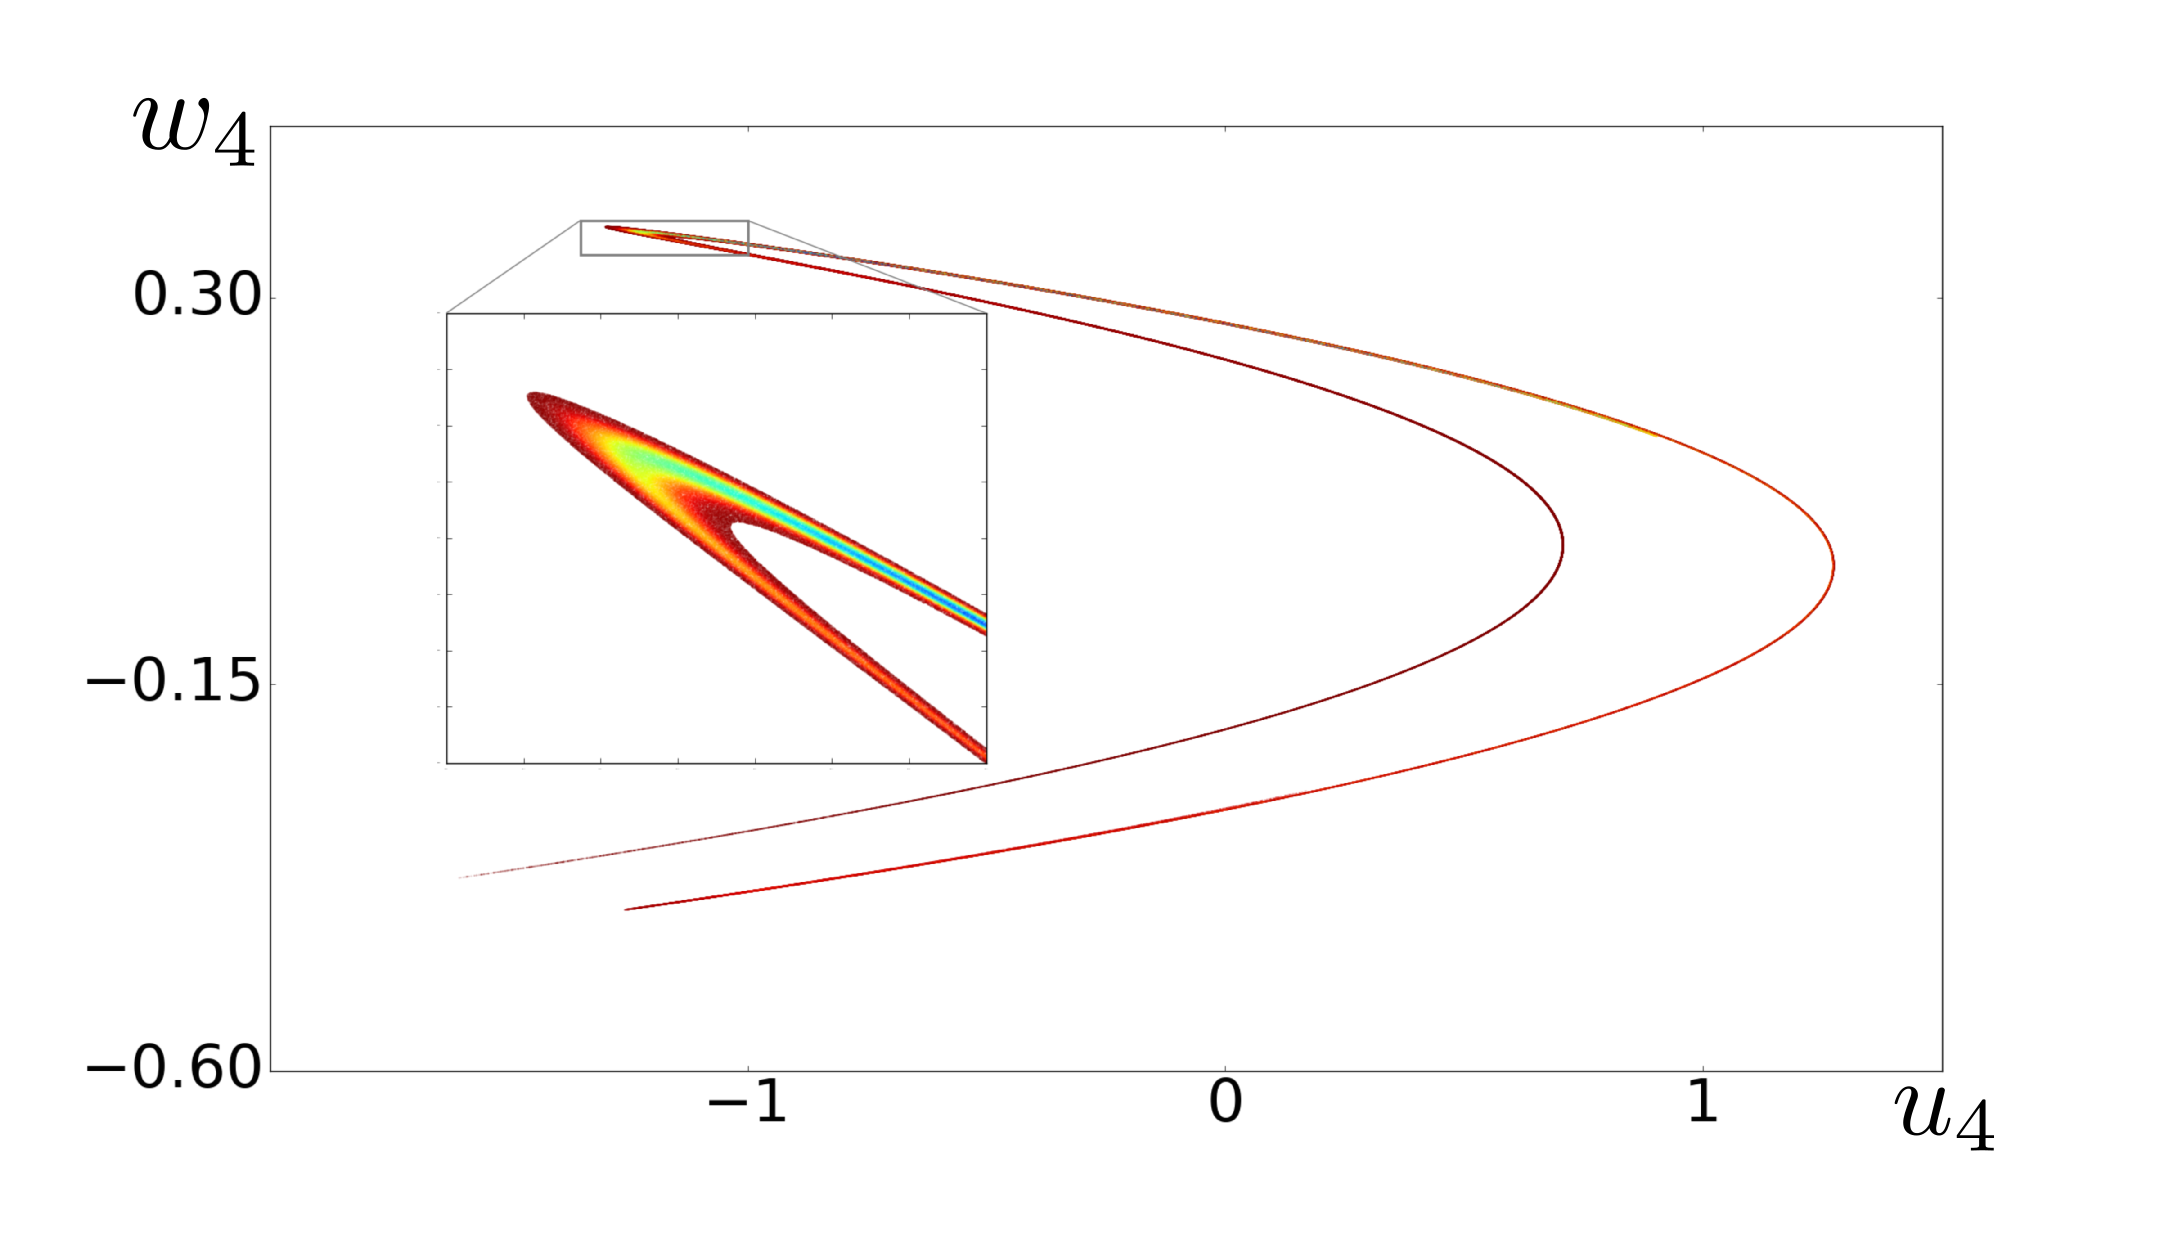
\includegraphics[width=\textwidth]{y4-x4-phi1}
    \subcaption{Coloring of $(u_4, w_4)$ samples by $\phi_1$, where
      $\phi_1$ is the result of DMAPS applied only to model
      responses.}
    \label{fig:test2}\par\vfill
    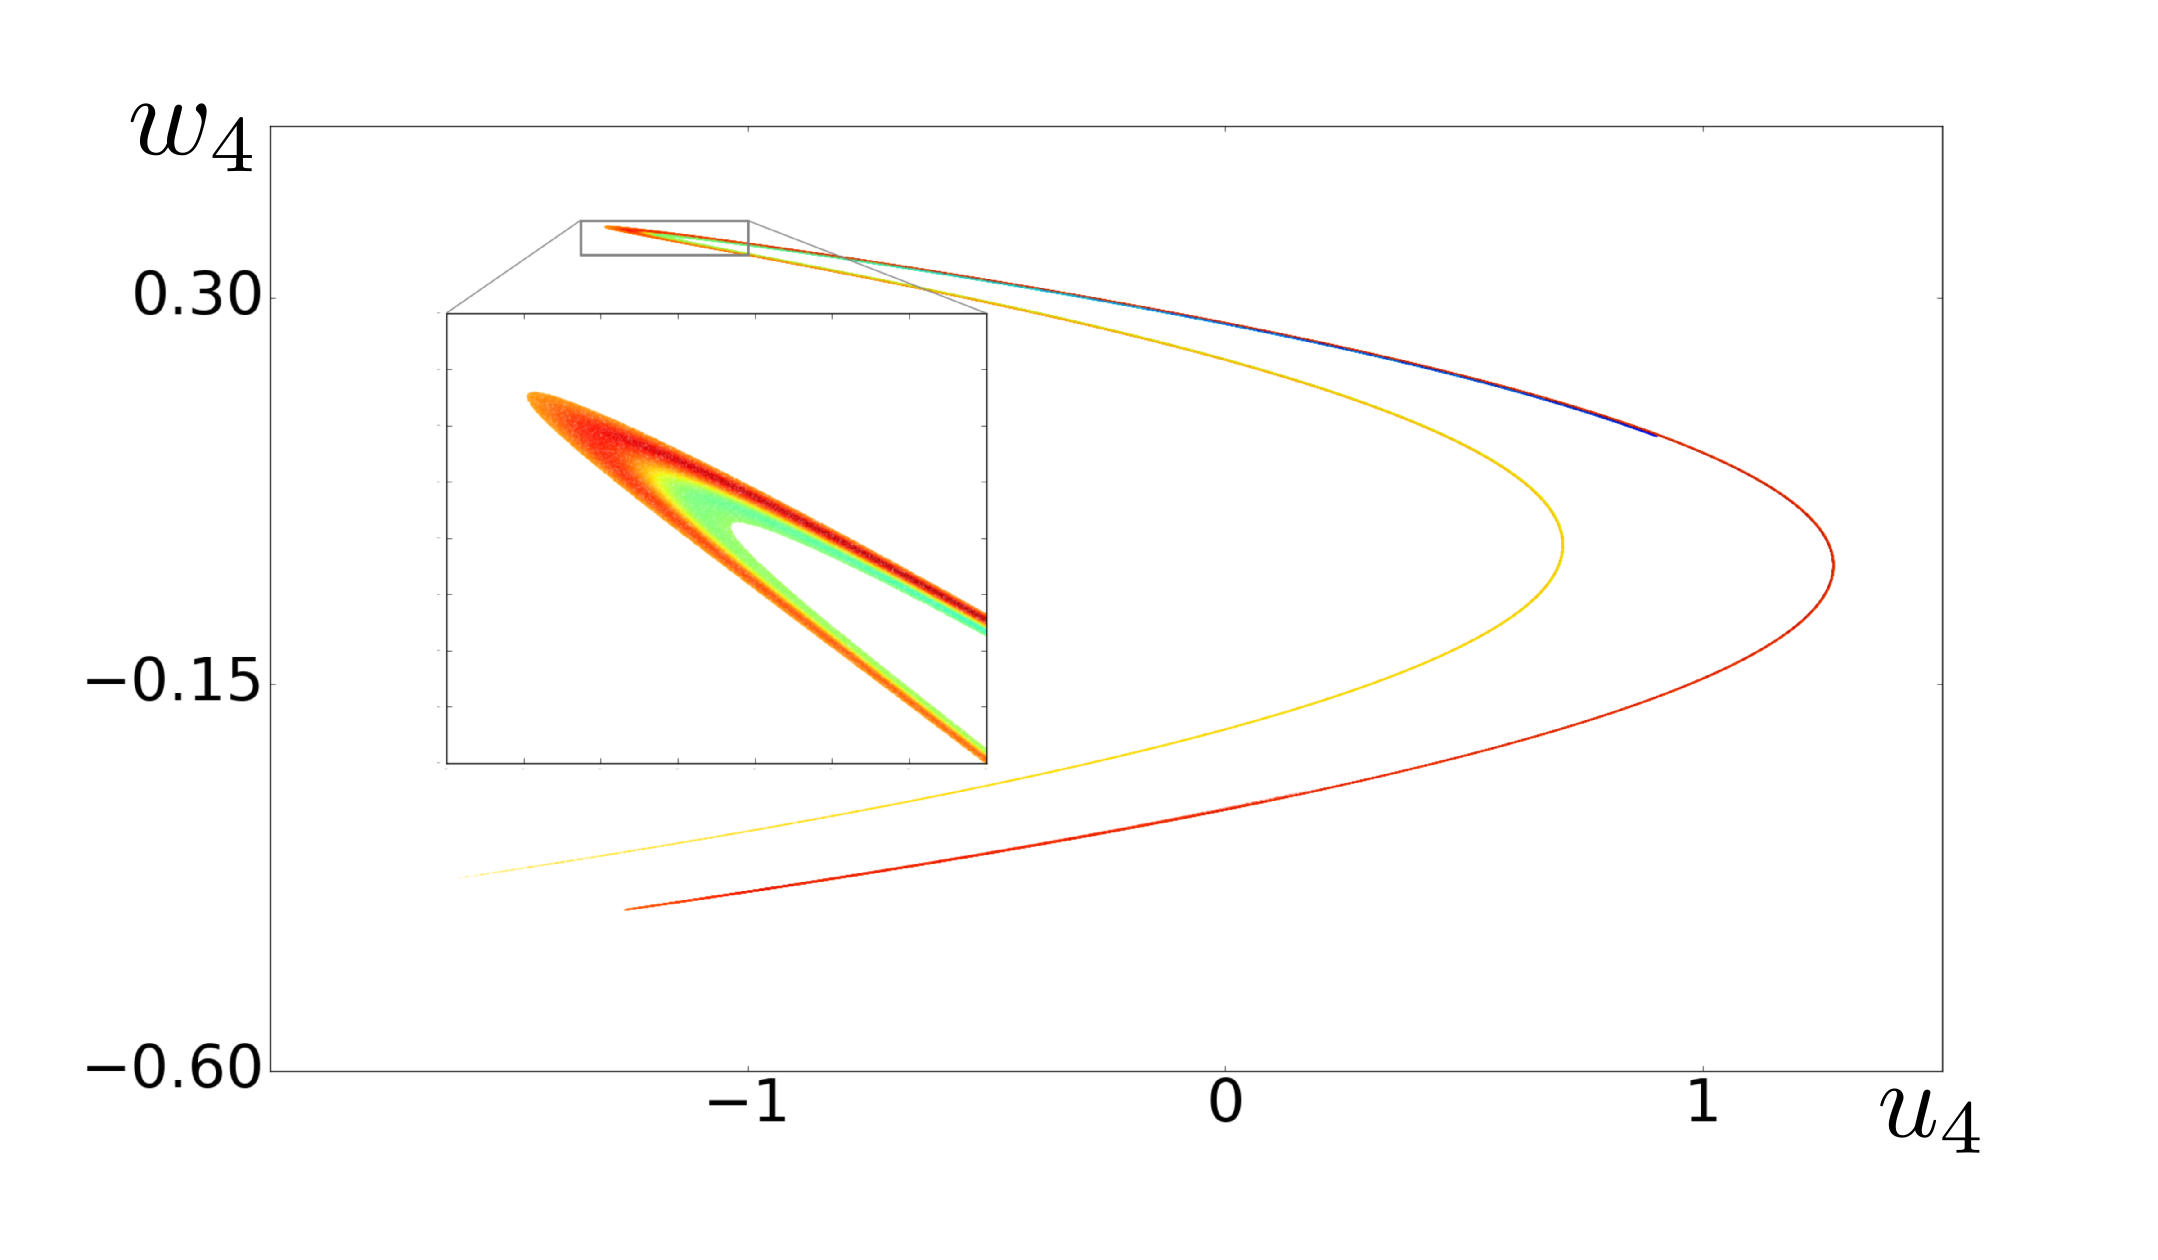
\includegraphics[width=\textwidth]{y4-x4-phi2}
    \subcaption{Coloring of $(u_4, w_4)$ samples by $\phi_2$, where
      $\phi_2$ is the result of DMAPS applied only to model
      responses.}
    \label{fig:test3}\par\vfill
  \end{minipage}
  \caption[Plot of modified DMAPS results on transformed model]{Result
    of applying modified kernel to transformed parameter problem,
    compare to
    Fig.~\ref{fig:henon-paramspace-dmaps}. \label{fig:henon-data-dmaps}
  }
\end{figure*}


Having shown that this modified DMAPS formulation holds potential in
uncovering effective parameters, we now present an application to a
more complex system.

\clearpage

\section{Application: Michaelis-Menten}

We apply our toolbox to a familiar chemical kinetic prototype, namely
the Michaelis--Menten--Henri system modeling enzymatic action.  In
that mechanism, a substrate $S$ is turned into product $P$ by the
action of an enzyme $E$ through the creation of an intermediate
complex $C$,

\begin{align}
 E + S \xrightleftharpoons[k_{-1}]{k_1} C \xrightarrow[]{k_2} E + P
. \label{mech:mm}
\end{align}

The mechanism differs from Mechanism~\ref{mech:abc} in that the
addition of a recycled but limited enzyme supply introduces
nonlinearities into the governing system of differential equations,


\begin{align}
  \begin{split}
    S' &= -k_1 E S + k_{-1} C , \\
    C' &= k_1 E S - (k_{-1} + k_2) C , \\
    E' &= -k_1 E S + (k_{-1} + k_2) C , \\
    P' &= k_2 C .
  \end{split}
\end{align}


The conservation laws $S + P + C = S_T$ and $E + C = E_T$ reduce the
number of variables by two, and we arrive at the final model

\begin{align}
  \begin{split}
    S' &= -k_1 (E_T-C) S + k_{-1} C , \\
    C' &= k_1 (E_T-C) S - (k_{-1} + k_2) C .
    \label{eq:MM}
  \end{split}
\end{align}

Following the classical setting \cite{MM13,SS89}, we set the initial
concentrations of complex and product to zero, $C_0=P_0=0$, so that
$S_0 = S_T$ and $E_0 = E_T$.  Further adapting ideas from \cite{SS89},
we recoordinatize the parameter space through the transformations

\begin{align}
  \begin{split}
    K_M = \frac{k_{-1} + k_2}{k_1} , &\quad
    V_M = k_2 E_T , \\
    \sigma = \frac{S_T}{K_M} , \quad \kappa =
    \frac{k_{-1}}{k_2} , &\quad \epsilon = \frac{E_T}{S_T +
      K_M} .
    \label{eq:param-defs}
  \end{split}
\end{align}

The observable here is the product concentration $P$ at ten equally
spaced times in the interval $[t_s/2,2t_s]$, where the timescale
$t_s = (S_T^* + K_M^*)/V_M^*$. Thus
$\mathbf{f}:\mathbb{R}^5 \rightarrow \mathbb{R}^{10}$ maps our five
parameter values to ten points along $P$'s trajectory. Setting
reference parameter values at
$(K_M^*,V_M^*,S_T^*,\epsilon^*,\kappa) = (1,1,1,10^{-3},10)$, we
investigate the system in a manner similar to that previously
presented.  First we sample parameter settings lying within a fixed
distance $\delta=0.05$ of
$\mathbf{f}^* = \mathbf{f}(K_M^*, V_M^*, S_T^*, \epsilon^*,
\kappa^*)$, and then we apply the modified DMAPS algorithm to that
dataset to uncover significant and sloppy parameter combinations.
Before delving into DMAPS, however, we first probe the system with a
simpler, linear PCA analysis.  By applying this technique to the
Jacobian of the model response

\begin{align}
  \mathrm{J} = \begin{bmatrix} \frac{\partial f_1}{\partial K_M} & \frac{\partial f_1}{\partial V_M} & \frac{\partial f_1}{\partial S_T} & \frac{\partial f_1}{\partial \epsilon} & \frac{\partial f_1}{\partial \kappa} \\ \vdots & & & & \vdots \\ \frac{\partial f_N}{\partial K_M} & & \hdots & & \frac{\partial f_N}{\partial \kappa} \end{bmatrix}
\end{align}

and examining the coefficients of the principal components
$\mathrm{V}$ where $\mathrm{J} = \mathrm{U \Sigma V^T}$, we will
uncover, in a local, linear sense, a basis for parameter space which
better captures the directions which do and do not affect model
output. This can be observed from the fact that
$\| \mathbf{f(p + \Delta p) - f(p)} \| \approx \| \mathrm{J}
\mathbf{\Delta p} \| = \| \mathrm{U \Sigma V^T} \mathbf{\Delta p}
\|$. When $\mathbf{\Delta p}$ aligns with a principal component whose
corresponding singular value is large, it will point in a direction of
significant model response variation. Conversely, a
$\mathbf{\Delta p}$ which aligns with a principal component whose
singular value is small will point in a sloppy direction along which
model response changes minimally. Examining the SVD of the Jacobian
evaluated at $\mathbf{p}^*$ we find for the principal components (with
entries less than $10^{-1}$ rounded to zero and singular values
rounded to the nearest order of magnitude for clarity)

\[
  V = \begin{blockarray}{cccccc} & v_1 & v_2 & v_3 & v_4 & v_5
    \\ \begin{block}{c[ccccc]} K_M & 0.3 & \minus 0.4 & \minus 0.9 & 0
      & 0 \\ V_M & \minus 0.4 & 0.8 & \minus 0.5 & 0 & 0 \\ S_T &
      \minus 0.9 & \minus 0.5 & 0 & 0 & 0 \\ \epsilon & 0 & 0 & 0 &
      0.9 & \minus 0.5 \\ \kappa & 0 & 0 & 0 & \minus 0.5 & \minus 0.9
      \\ \end{block} & & & & & \\ \begin{block}{c[ccccc]} \sigma &
      10^0 & 10^0 & 10^{\minus 2} & 10^{\minus 5} & 10^{\minus 6}
      \\ \end{block} \end{blockarray}
\]

where the final row labeled $\sigma$ contains the corresponding singular values. This simple analysis immediately suggests the existence of two sloppy parameters in this regime, $\kappa$ and $\epsilon$, as the principal components that span these axes correspond to significantly smaller singular values compared to the other vectors. In addition, it appears that the parameter space direction $K_M = V_M$ may be sloppy as this approximately corresponds to the third smallest principal component, singular value pair. With this simple analysis in hand, we turn to computational verification of the results using both direct numerical experiments and the DMAPS scheme outlined above, along with supporting analytical arguments.

First we show that the direction $K_M = V_M$ is indeed sloppy so that one cannot precisely determine both $K_M$ and $V_M$, but only their ratio. To do so we turn to the Lineweaver-Burk plot, a graphical procedure allowing one to determine $K_M$ and $V_M$ from experimental data of the reaction rate and substrate concentration evolution over time \ref{LB}. By generating many noisy realizations of the product concentration profiles as one might collect experimentally in the lab and then fitting each with the Lineweaver-Burk method, we can observe the range of predicted $K_M$, $V_M$ pairs. These results are plotted in Fig.~\ref{fig:lb}. In a typical setting we would expect a spread of predicted values centered around the true, zero-noise parameters taking the shape of some ellipsoid. However, as we have seen in previous examples, in the presence of sloppiness this ellipsoid would be stretched out along the sloppy parameter direction. This is precisely what we find in Fig.~\ref{fig:lb}: so long as the ratio $K_M/V_M = K_M^*/V_M^* = 1$, a wide range of values provide best-fit parameters in the presence of slight noise. Therefore, when fitting parameters in this regime, we must accept that we may not be able to determine precise values of both $K_M$ and $V_M$.


\begin{figure}
  \centering
  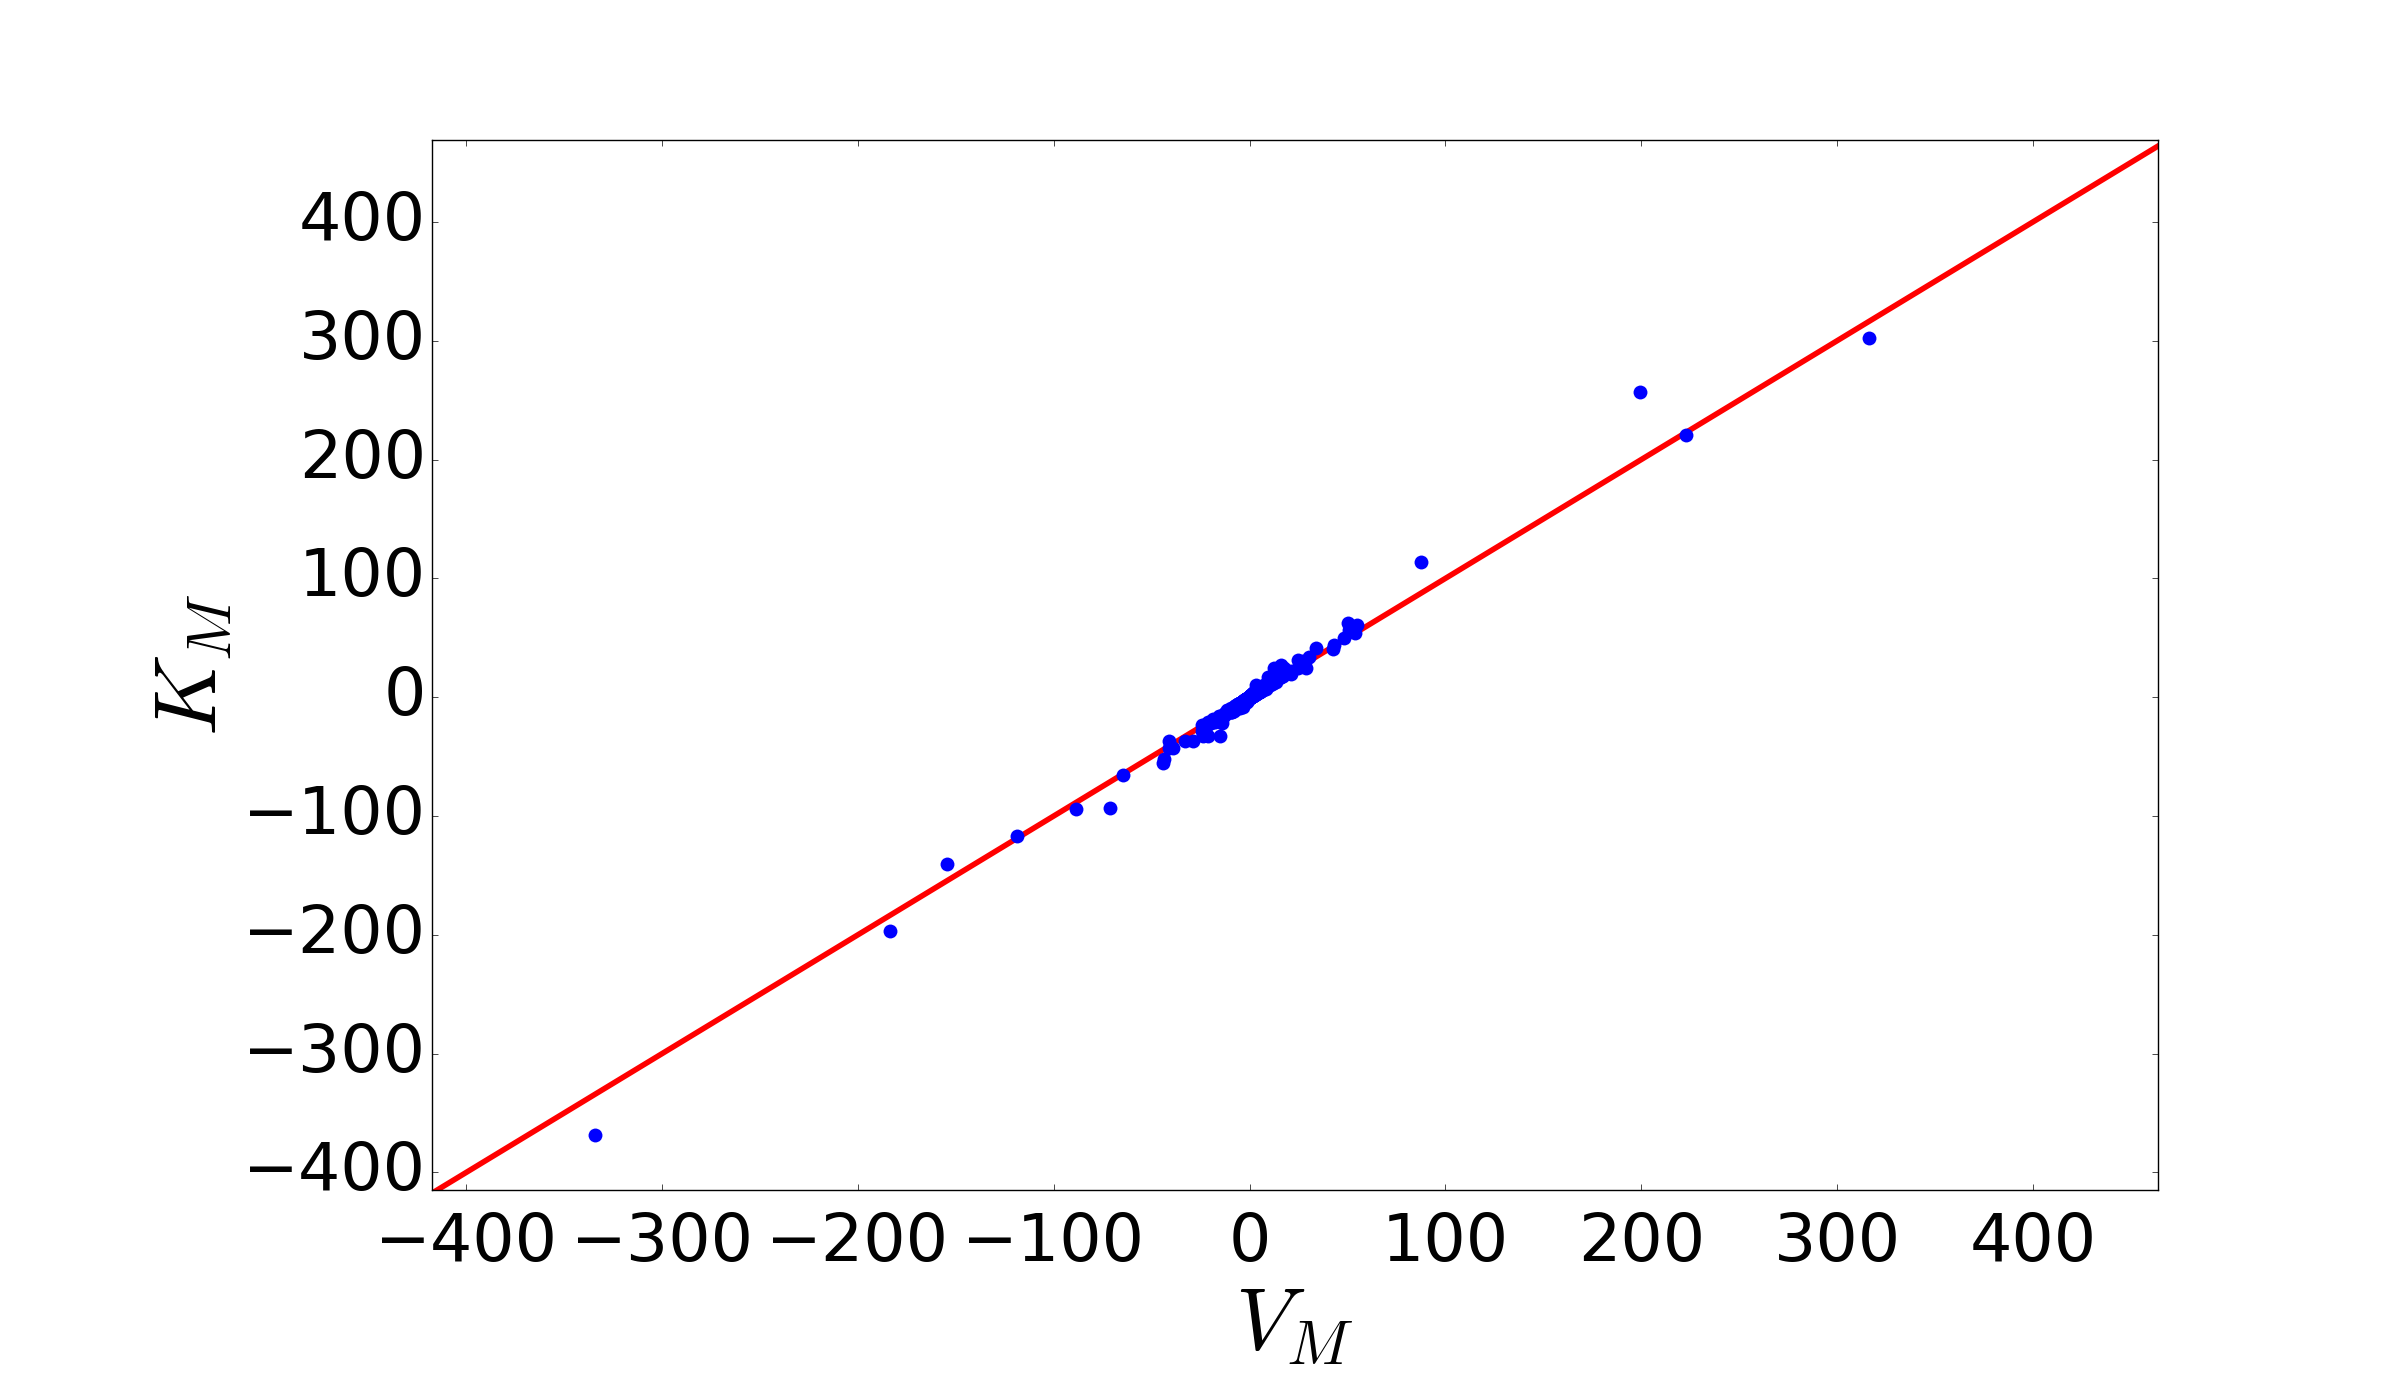
\includegraphics[width=1.0\linewidth]{k-v-lb}
  \caption[Illustration of sloppiness in Lineweaver-Burk fitting]{Best
    fit $K_M$ and $V_M$ values for many noisy concentration
    trajectories (blue dots). Sloppiness is evident in the spread of
    the data along the line $K_M/V_M = 1$ (plotted in red for
    reference). \label{fig:lb} }
\end{figure}

Next, we examine the system using DMAPS. We use the five-dimensional dataset obtained by asampling parameter space around $\mathbf{p}^*$ and keeping those points for which $\|\mathbf{f(p) - f(p^*)} || < 5  \cdot 10^{-2}$, and apply the modified DMAPS given in \eqref{eq:dmaps-w-mod} with an $\epsilon$ and $\lambda$ value of $10^{2}$ and $10^{-1}$ respectively.

Having computed our DMAP eigenvectors, it remains to determine which
of them correspond to independent directions in parameter space, as
certain eigenvectors may parameterize the same directions (see
\ref{carmeline} for details). Using the algorithm developed in
\ref{carmeline}, we compute a residual for each eigenvector which,
roughly speaking, assesses how much new information it contains. The
results shown in Fig~\ref{fig:resids} suggest that eigenvectors
$\phi_1$, $\phi_2$, $\phi_6$ and $\phi_7$ all parameterize independent
directions. By design, \eqref{eq:dmaps-w-mod} will return eigenvectors
tracking important parameter directions first, with sloppy directions
following. Our previous analysis would then suggest that $\phi_1$ and
$\phi_2$ correspond to important parameter directions, while $\phi_6$
and $\phi_8$ correspond to sloppy directions. $\phi_5$, lying in the
middle, may contain components of both sloppy and  important
directions. Therefore, we would expect $\phi_1$ and $\phi_2$ to
provide a good set of coordinates on our model manifold, while
$\phi_6$ and $\phi_8$ would not correspond to meaningful directions in
model space.

We can test this hypothesis by projecting the model manifold onto two
axes, here $f_1$ and $f_{10}$, and coloring the result by our
eigenvectors. If the colors vary smoothly over the points, we have
uncovered an eigenvector that parameterizes the manifold. Otherwise,
the eigenvector will correspond to a sloppy direction. These colorings
are provided in Fig.~\ref{fig:mm-phis}. Based on these figures, we can
conclude that indeed $\phi_1$ and $\phi_2$ provide coordinates along
the model manifold, while the remaining eigenvectors do not correspond
to meaningful directions in model response space. However, by coloring
the $(\epsilon, \kappa)$ plane by $\phi_6$ and $\phi_7$ as in
Fig.~\ref{fig:ek-67} we find that these eigenvectors parameterize the
sloppiness in our model as hypothesized. The sloppiness in $K_M/V_M$
was discussed in the previous paragraph, but it remains to show why
$\epsilon$ and $\kappa$ should be difficult to estimate. In fact, as
$\epsilon \rightarrow 0$, the set of differential equations given in
\eqref{eq:MM} become singularly perturbed. In this limit, the leading
order dynamics are not influenced by $\kappa$ (see
Appendix~(\ref{app:MM}) for details). Thus, for small enough
$\epsilon$, we will lose our ability to determine both $\epsilon$ and
$\kappa$. This is precisely what is reflected in our DMAPS results. In
summary, a single application of our modified DMAPS algorithm
uncovered both important and sloppy directions in our model without
recourse to the underlying analytical system of equations.

\begin{figure*}
  \centering
  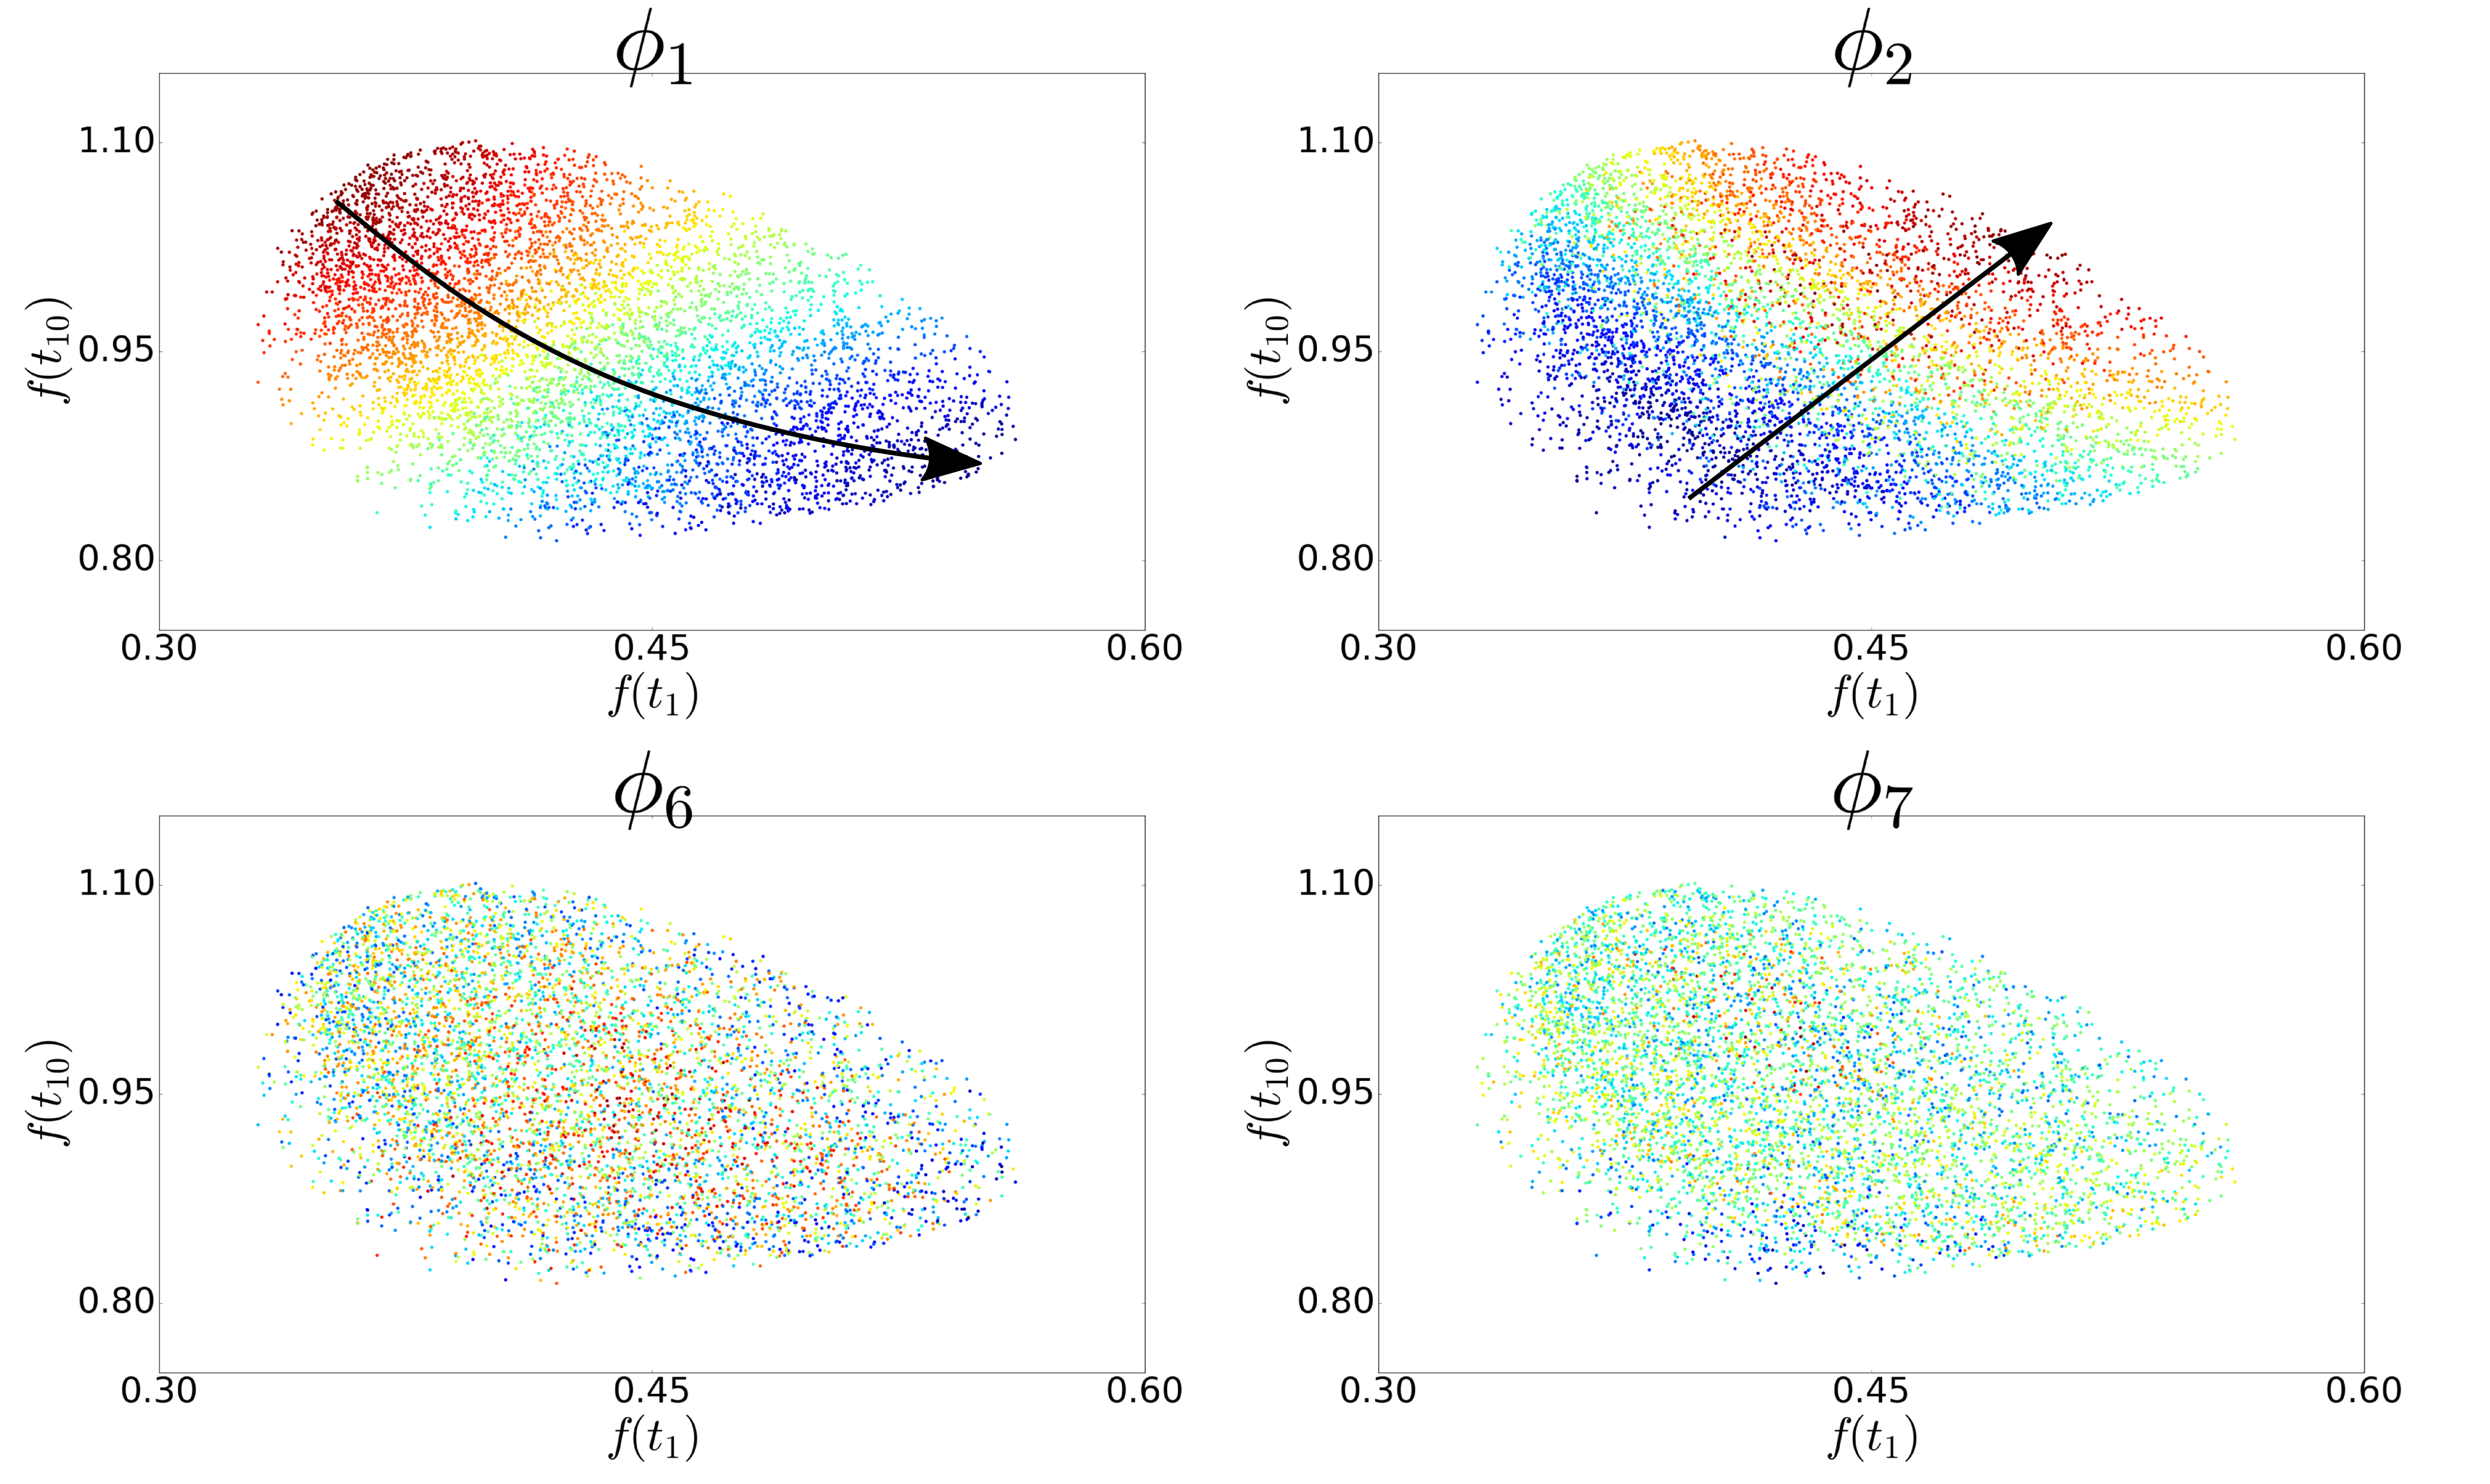
\includegraphics[width=1.0\linewidth]{mm-phis}
  \caption[Modified DMAPS embeddings of model manifold]{Projection of
    the model manifold onto $f_1$ and $f_{10}$ colored by different
    DMAP eigenvectors. As $\phi_1$ and $\phi_2$ vary smoothly over the
    surface and parameterize independent directions, these
    eigenvectors offer a good pair of coordinates on the manifold. On
    the other hand, $\phi_6$ and $\phi_7$ are scattered randomly over
    the surface. \label{fig:mm-phis} }
\end{figure*}

\begin{figure*}
  \centering
  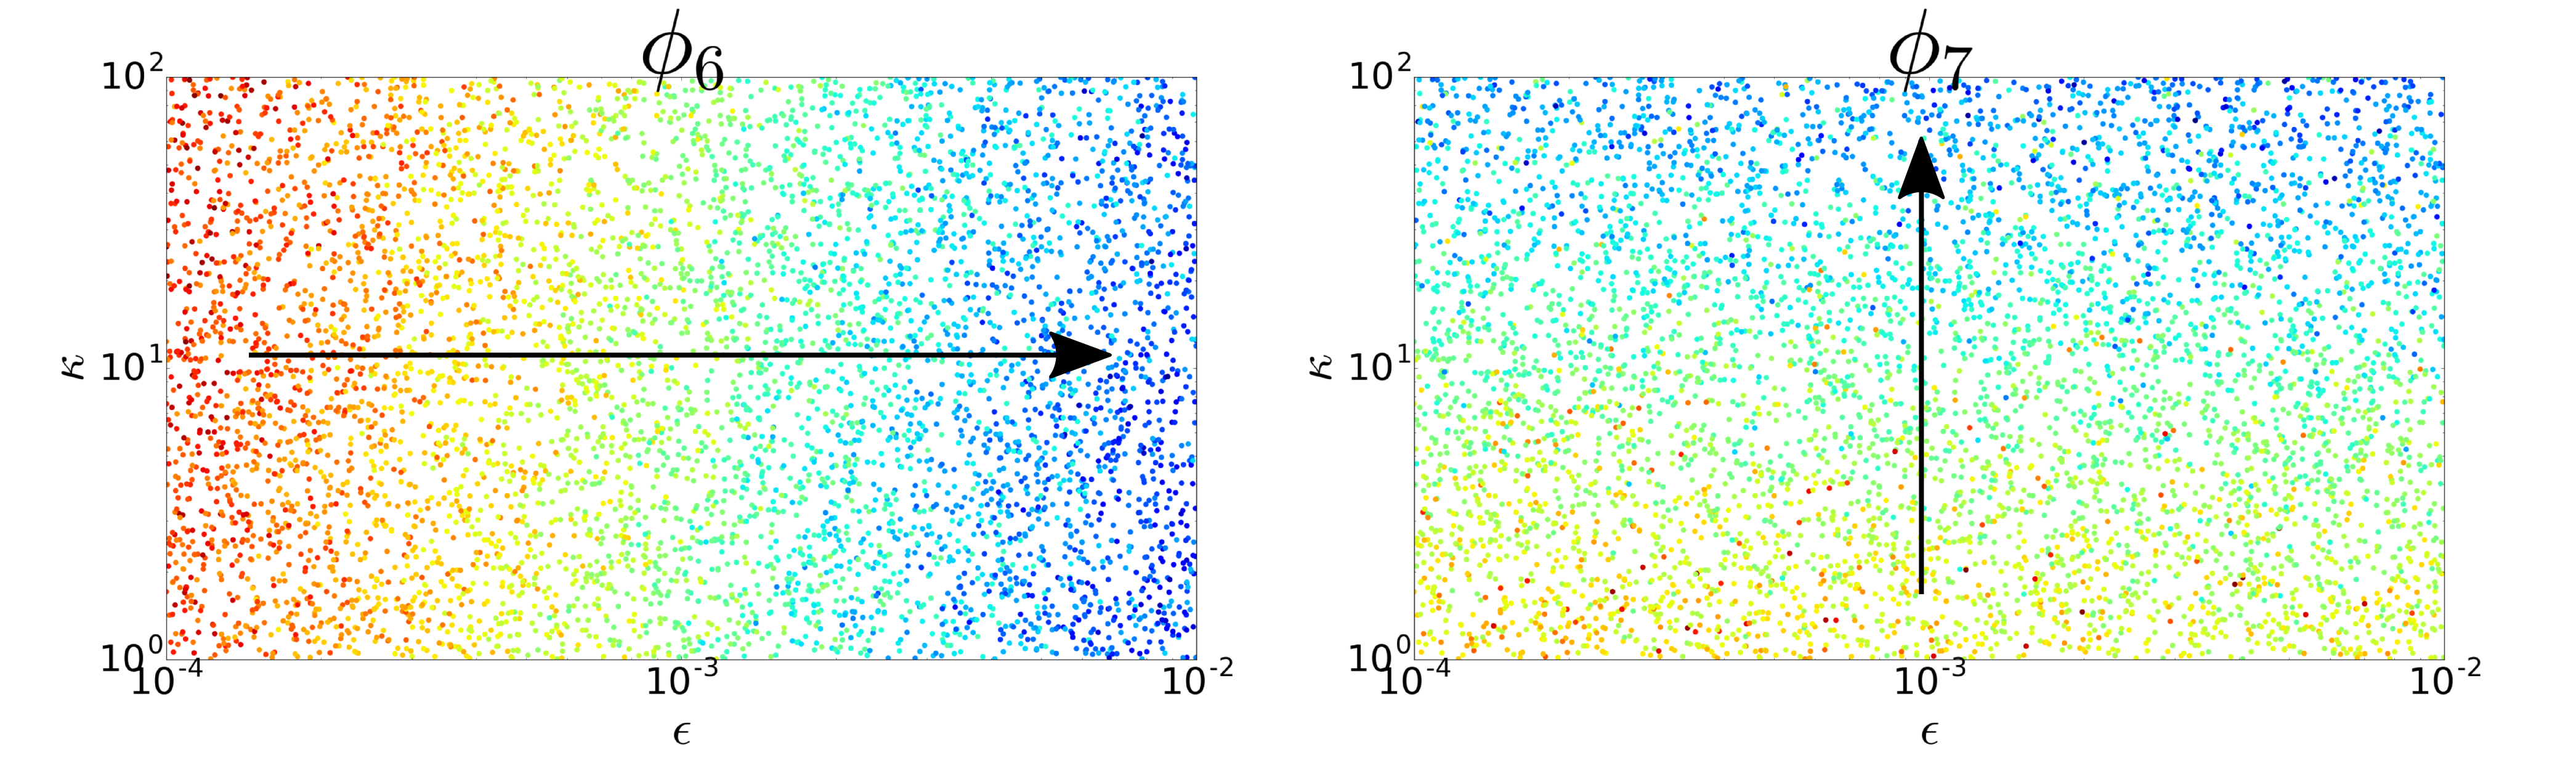
\includegraphics[width=1.0\linewidth]{kappa-eps-phis}
  \caption[Modified DMAPS embeddings of parameter space]{Coloring of
    the $(\epsilon, \kappa)$ plane by $\phi_6$ and $\phi_7$. While
    these eigenvectors were randomly distributed over the model
    manifold (Fig.~\ref{fig:mm-phis}), they neatly parameterize this
    plane, and thus capture the sloppy parameters in our
    model. \label{fig:ek-67} }
\end{figure*}

\begin{figure*}[ht!]
  \centering
  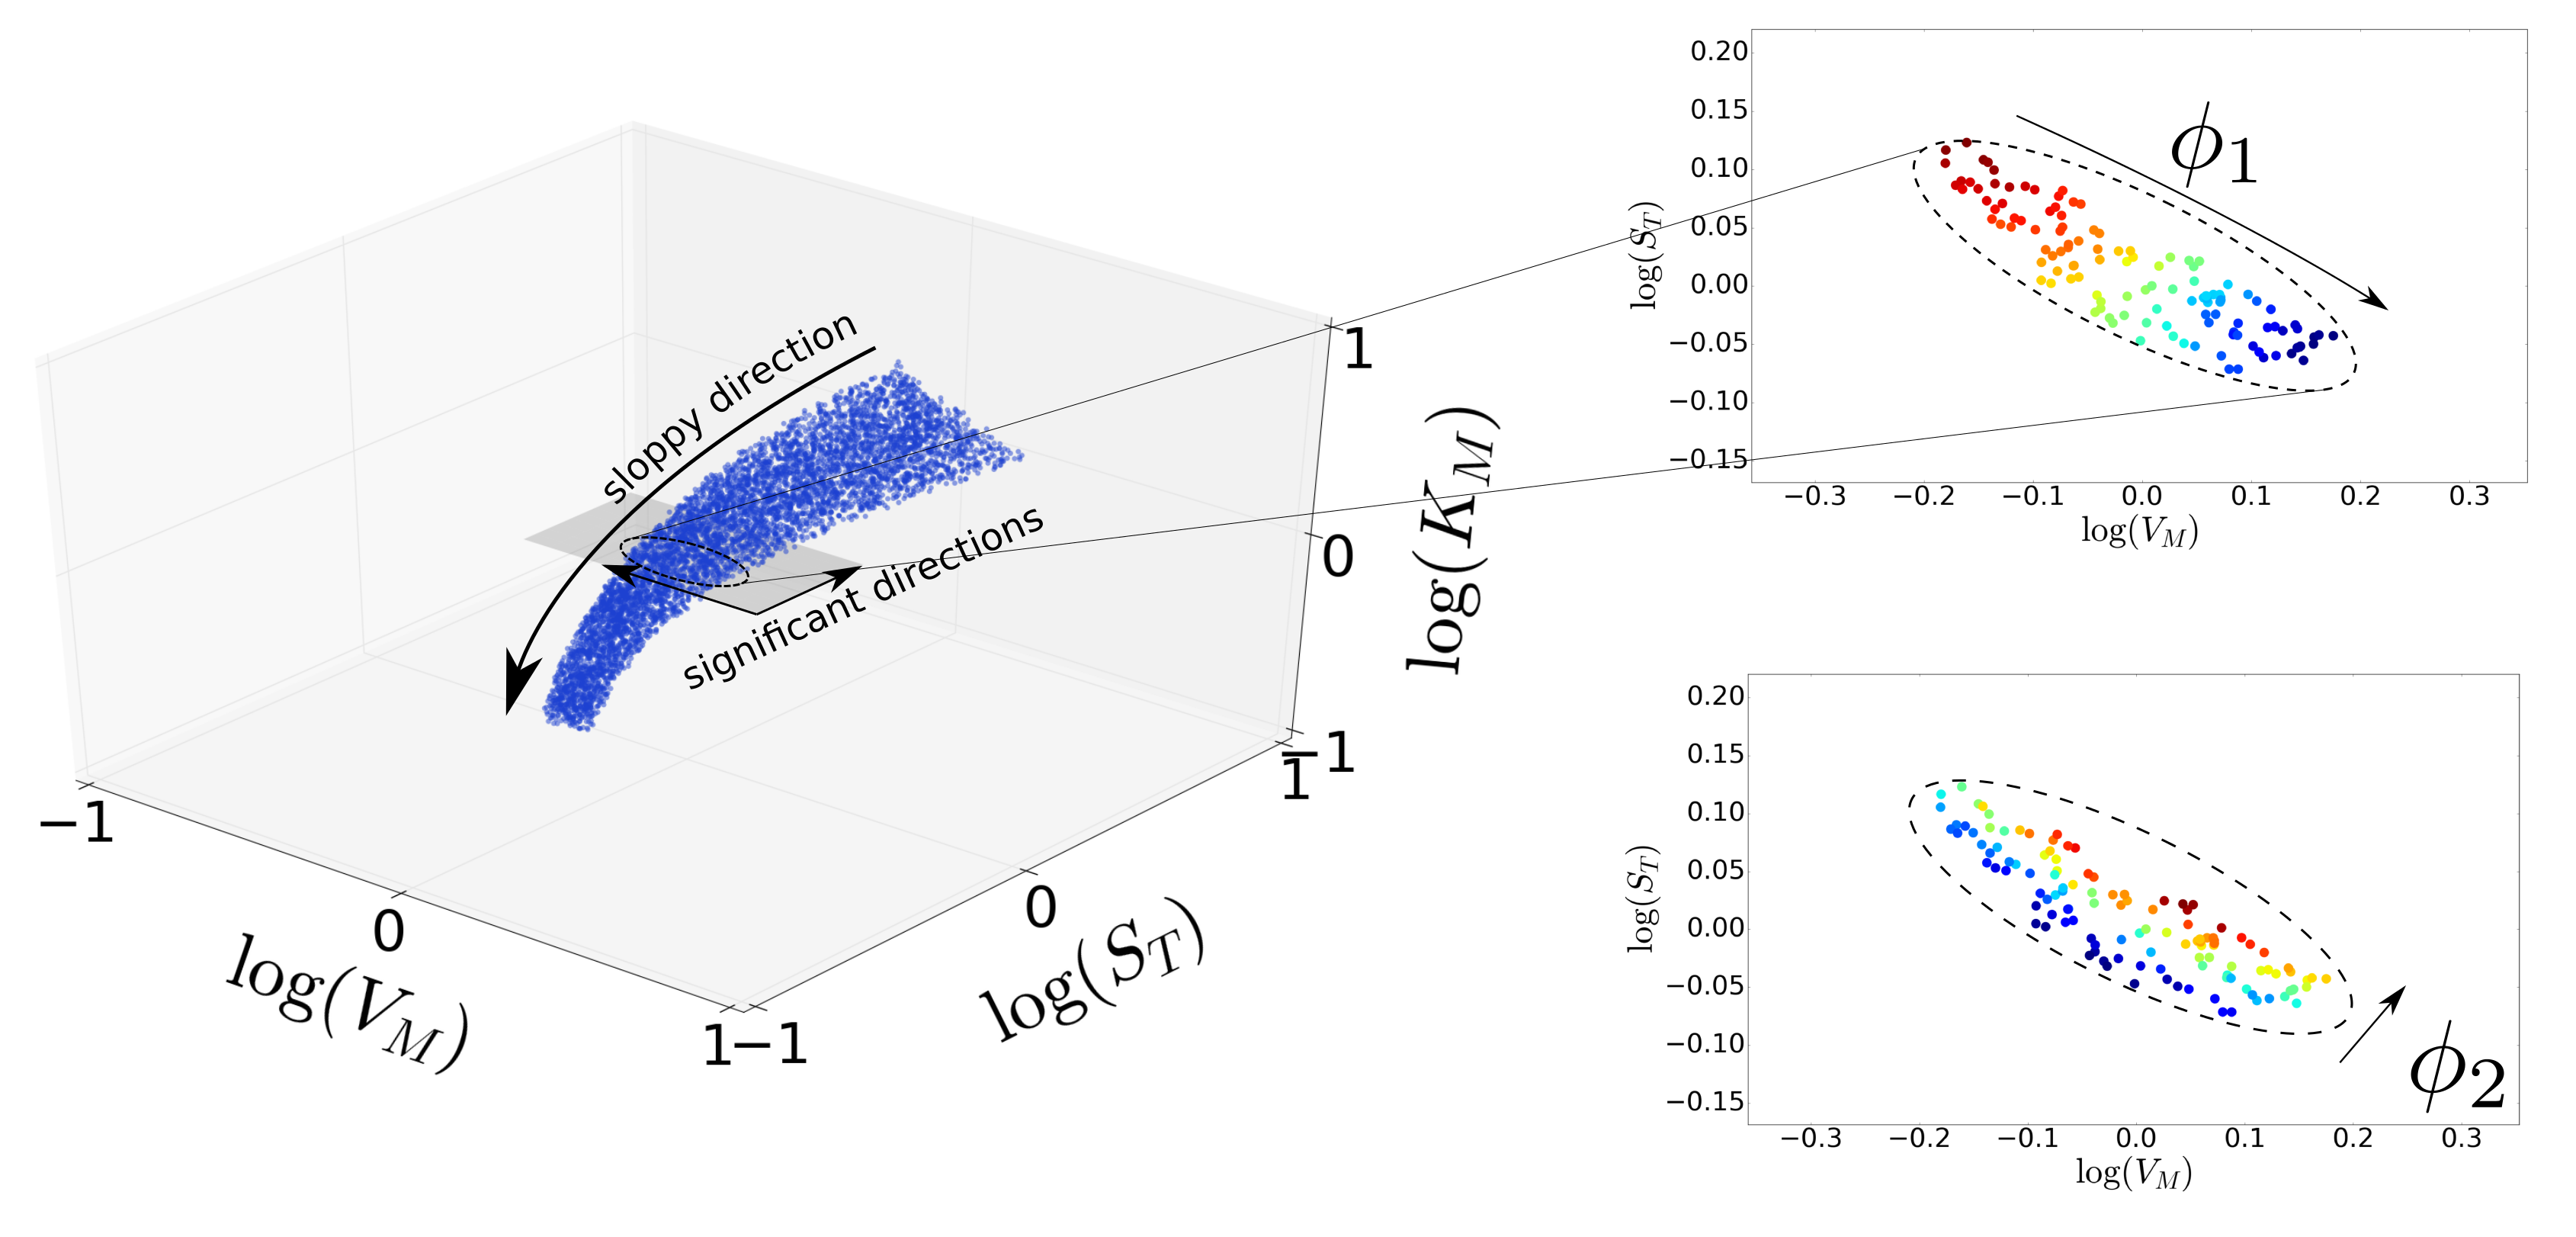
\includegraphics[width=\textwidth]{vm-st-km-all}
  \caption[Another view of the modified DMAPS embeddings of parameter
  space]{(left) Scatter-plot of points in parameter space such that
    $\|f(\theta) - f^*\| < \delta$. This reveals a sloppy direction
    corresponding to the long, curved axis, and two significant
    directions orthogonal to it. (right) Two-dimensional cross section
    colored by $\phi_1$ and $\phi_2$. As expected, these eigenvectors
    do parameterize the significant directions in parameter space. 
    \label{fig:vsk-dd} }
\end{figure*}

\clearpage

Finally, we mention that the definition of $\epsilon$ presented in
\eqref{eq:param-defs} that has been used throughout this section is a
revised definition based on the work in \ref{SegelSlemrod}. There,
they show that the previous definition of $\epsilon^* = E_T/S_T$ was
not sufficiently general, and that $\epsilon = E_T/(K_M + S_T)$
provides a more accurate description of the regions of parameter space
in which the system is singularly perturbed. We confirm this by
examining the model manifold at small $\epsilon^*$ and $\epsilon$,
which can be chosen independently by fixing $E_T$, $k_{-1}$ and $k_2$
in the original parameterization and adjusting $S_T$ and $k_1$ to
achieve the desired values of $\epsilon^*$ and $\epsilon$. In this way
we sample the $(\epsilon, \epsilon^*)$ plane and take as model
response $f(\theta) = \big(P(t_1), P(t_2) \big)$ with $t_1 = t_s/2$
and $t_2 = 2 t_s$. Applying the modified DMAP algorithm to the
resulting dataset yields the embedding shown in Fig.~\ref{fig:MM-ss},
with points in parameter space shown on the left (note that
$\epsilon > \epsilon^*$ implies $S_T < 0$ which is not physically
meaningful, so all points satisfy $\epsilon \leq \epsilon^*$). If we
had not discovered the extended region of singular perturbation
implied by the new definition of $\epsilon$, we would expect that all
samples fall in a region of two-dimensional model response (i.e. no
singular perturbation and thus no reduction in the number of variables
required to describe the system). However, our data-driven procedure
reveals what we had previously discovered through analytical
investigation: that there is in fact a region in which the system is
singularly perturbed, and therefore sloppy, despite having moderate
values of $\epsilon^*$. We show this as an example of DMAPS' ability
to reveal different regions of parameter space without recourse to
analytical investigation of the underlying equations, which is the
main strength of the technique presented here. All that was required
was a black-box function returning the model response at given
parameter settings. This is the main strength of the technique
presented here.

% We would expect that at small $\epsilon^*$ the system is singularly
% perturbed, and thus the determinant of the Jacobian of the model
% response would be small, suggesting that this region of parameter
% space is mapped to a small area of the model manifold and is
% therefore sloppy. However, we would also expect to find a region of
% moderate $\epsilon^*$ but small $\epsilon$ where $K_M \gg 1$ that
% likewise leads to a small determinant, suggesting the expanded
% definition does indeed broaden the region of parameter space in
% which the system is singularly perturbed and
% sloppy. Fig.~\ref{fig:MM-ss} confirms this is the case by plotting
% both parameter space and the corresponding model manifold colored by
% $\log(\mathrm{J_f})$.

\begin{figure*}
  \centering
  \begin{subfigure}[t]{0.45\linewidth}
    \centering
    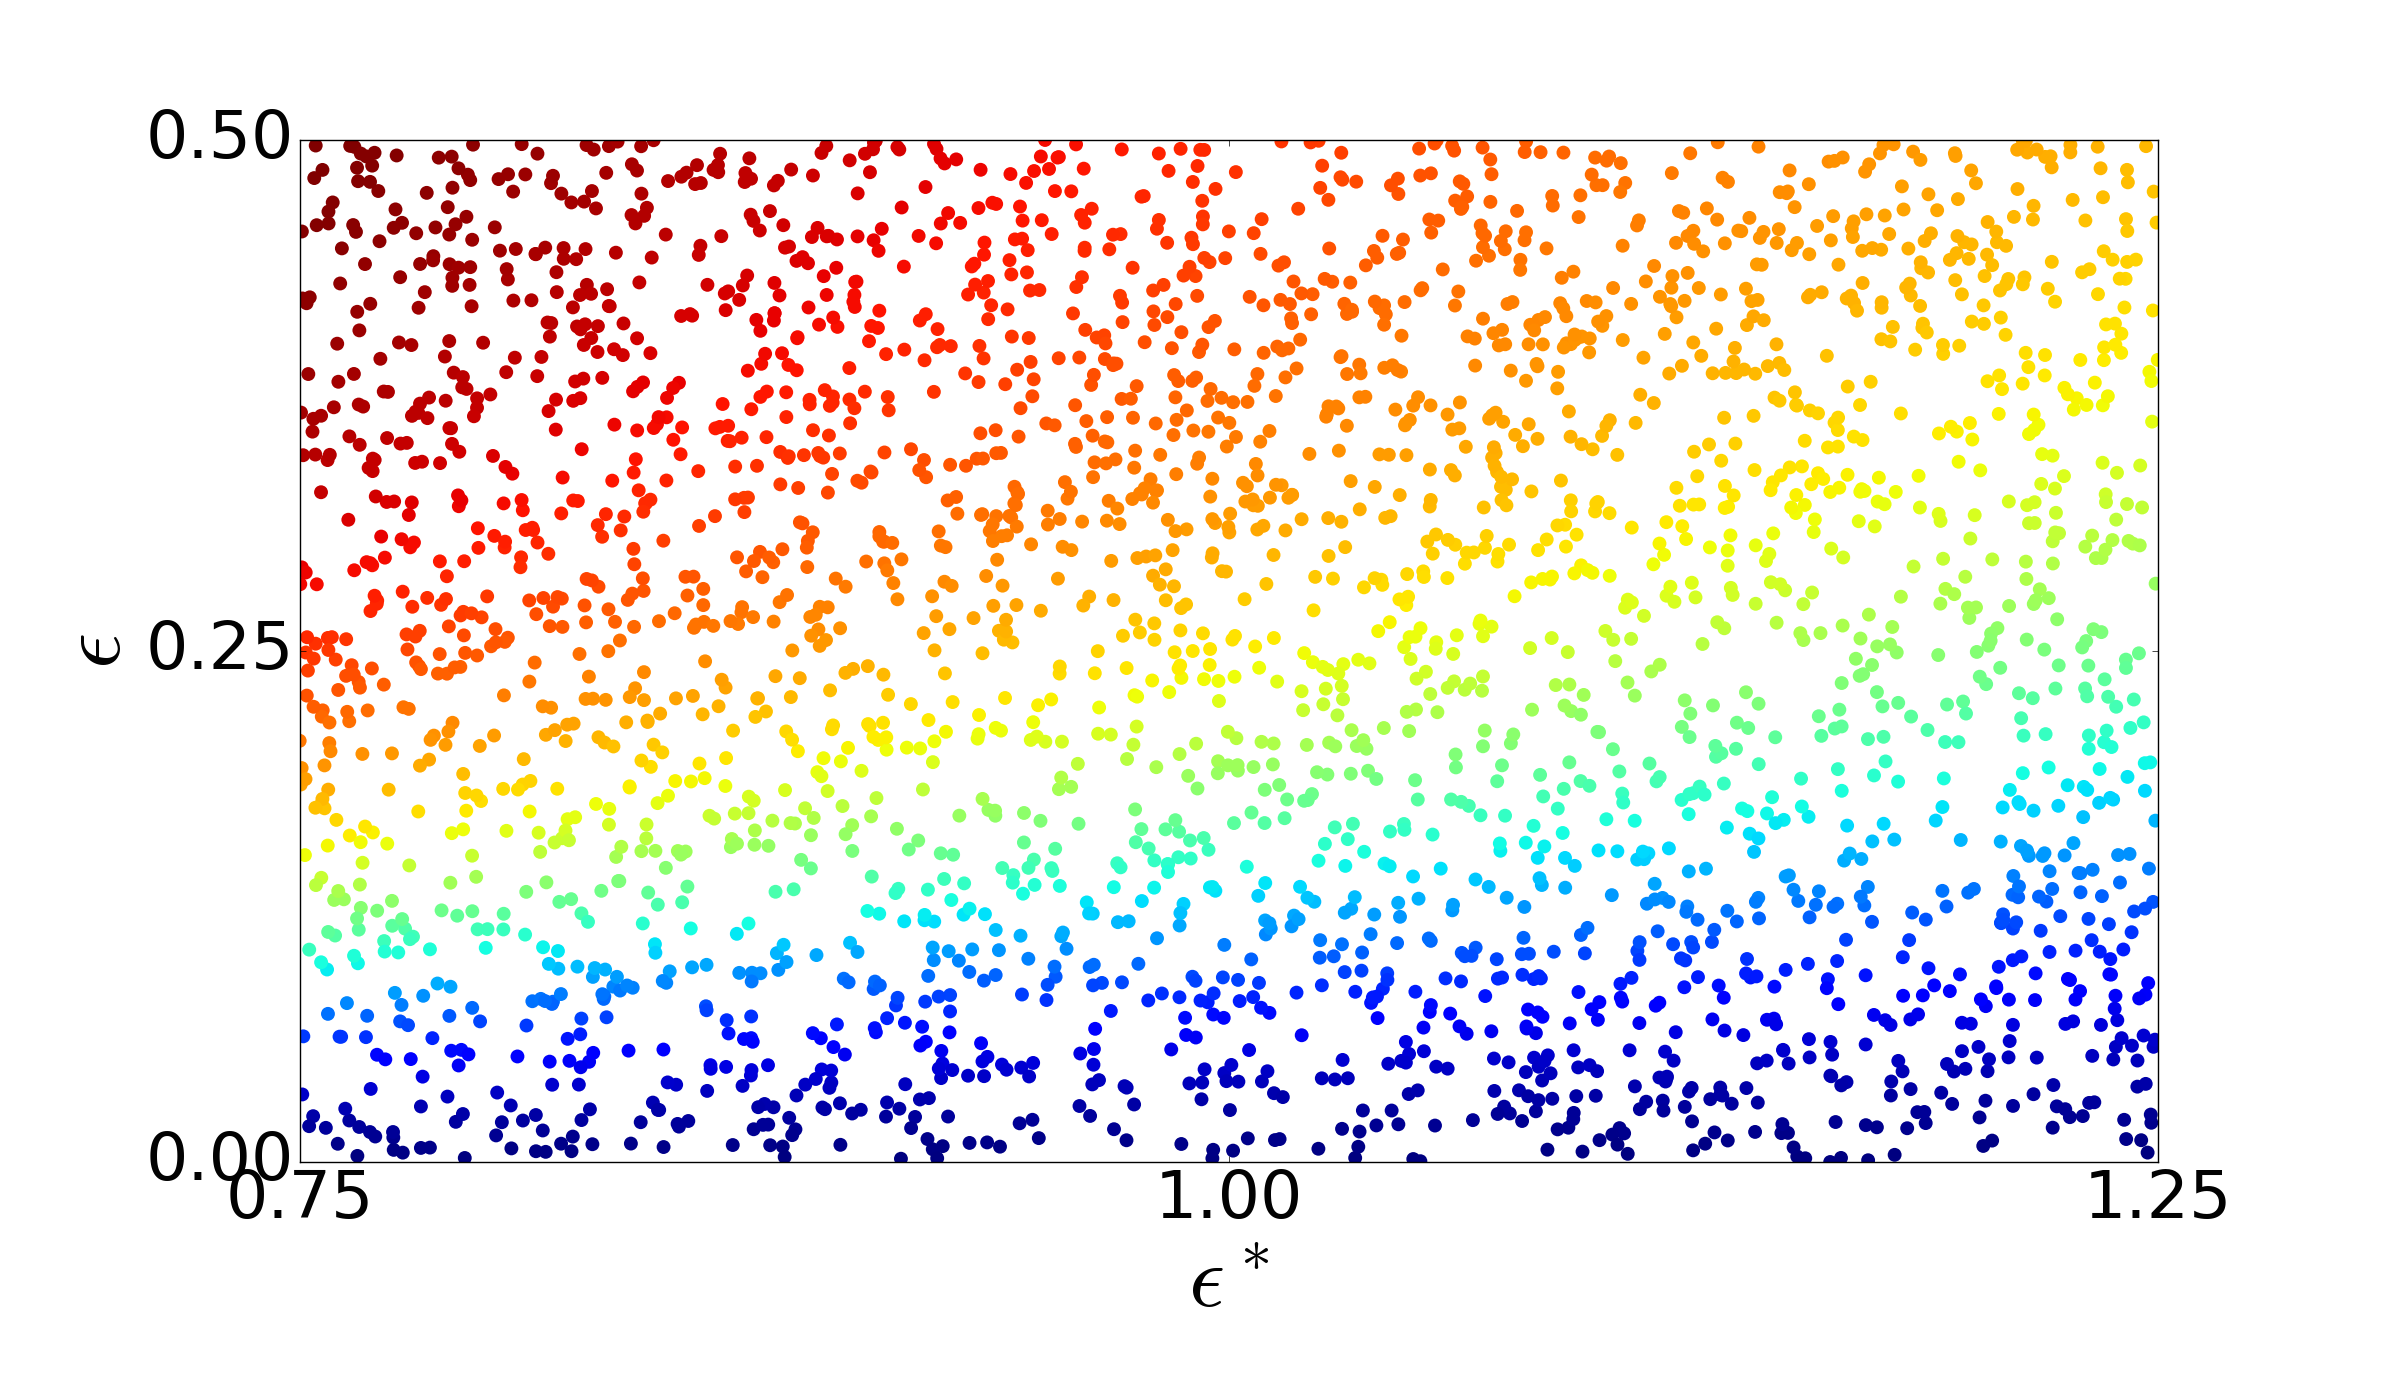
\includegraphics[width=1.0\linewidth]{eps-epsstar-phi1}
    \subcaption{Coloring of $(\epsilon, \epsilon^*)$ by the
      determinant of the model response Jacobian. Small values
      indicate a compression of parameter space which is indicative of
      mode sloppiness. Thus we see that at both small $\epsilon$ and
      small $\epsilon^*$ the system exhibits sloppiness.}
  \end{subfigure}
  \hspace{0.5cm}
  \begin{subfigure}[t]{0.45\linewidth}
    \centering
    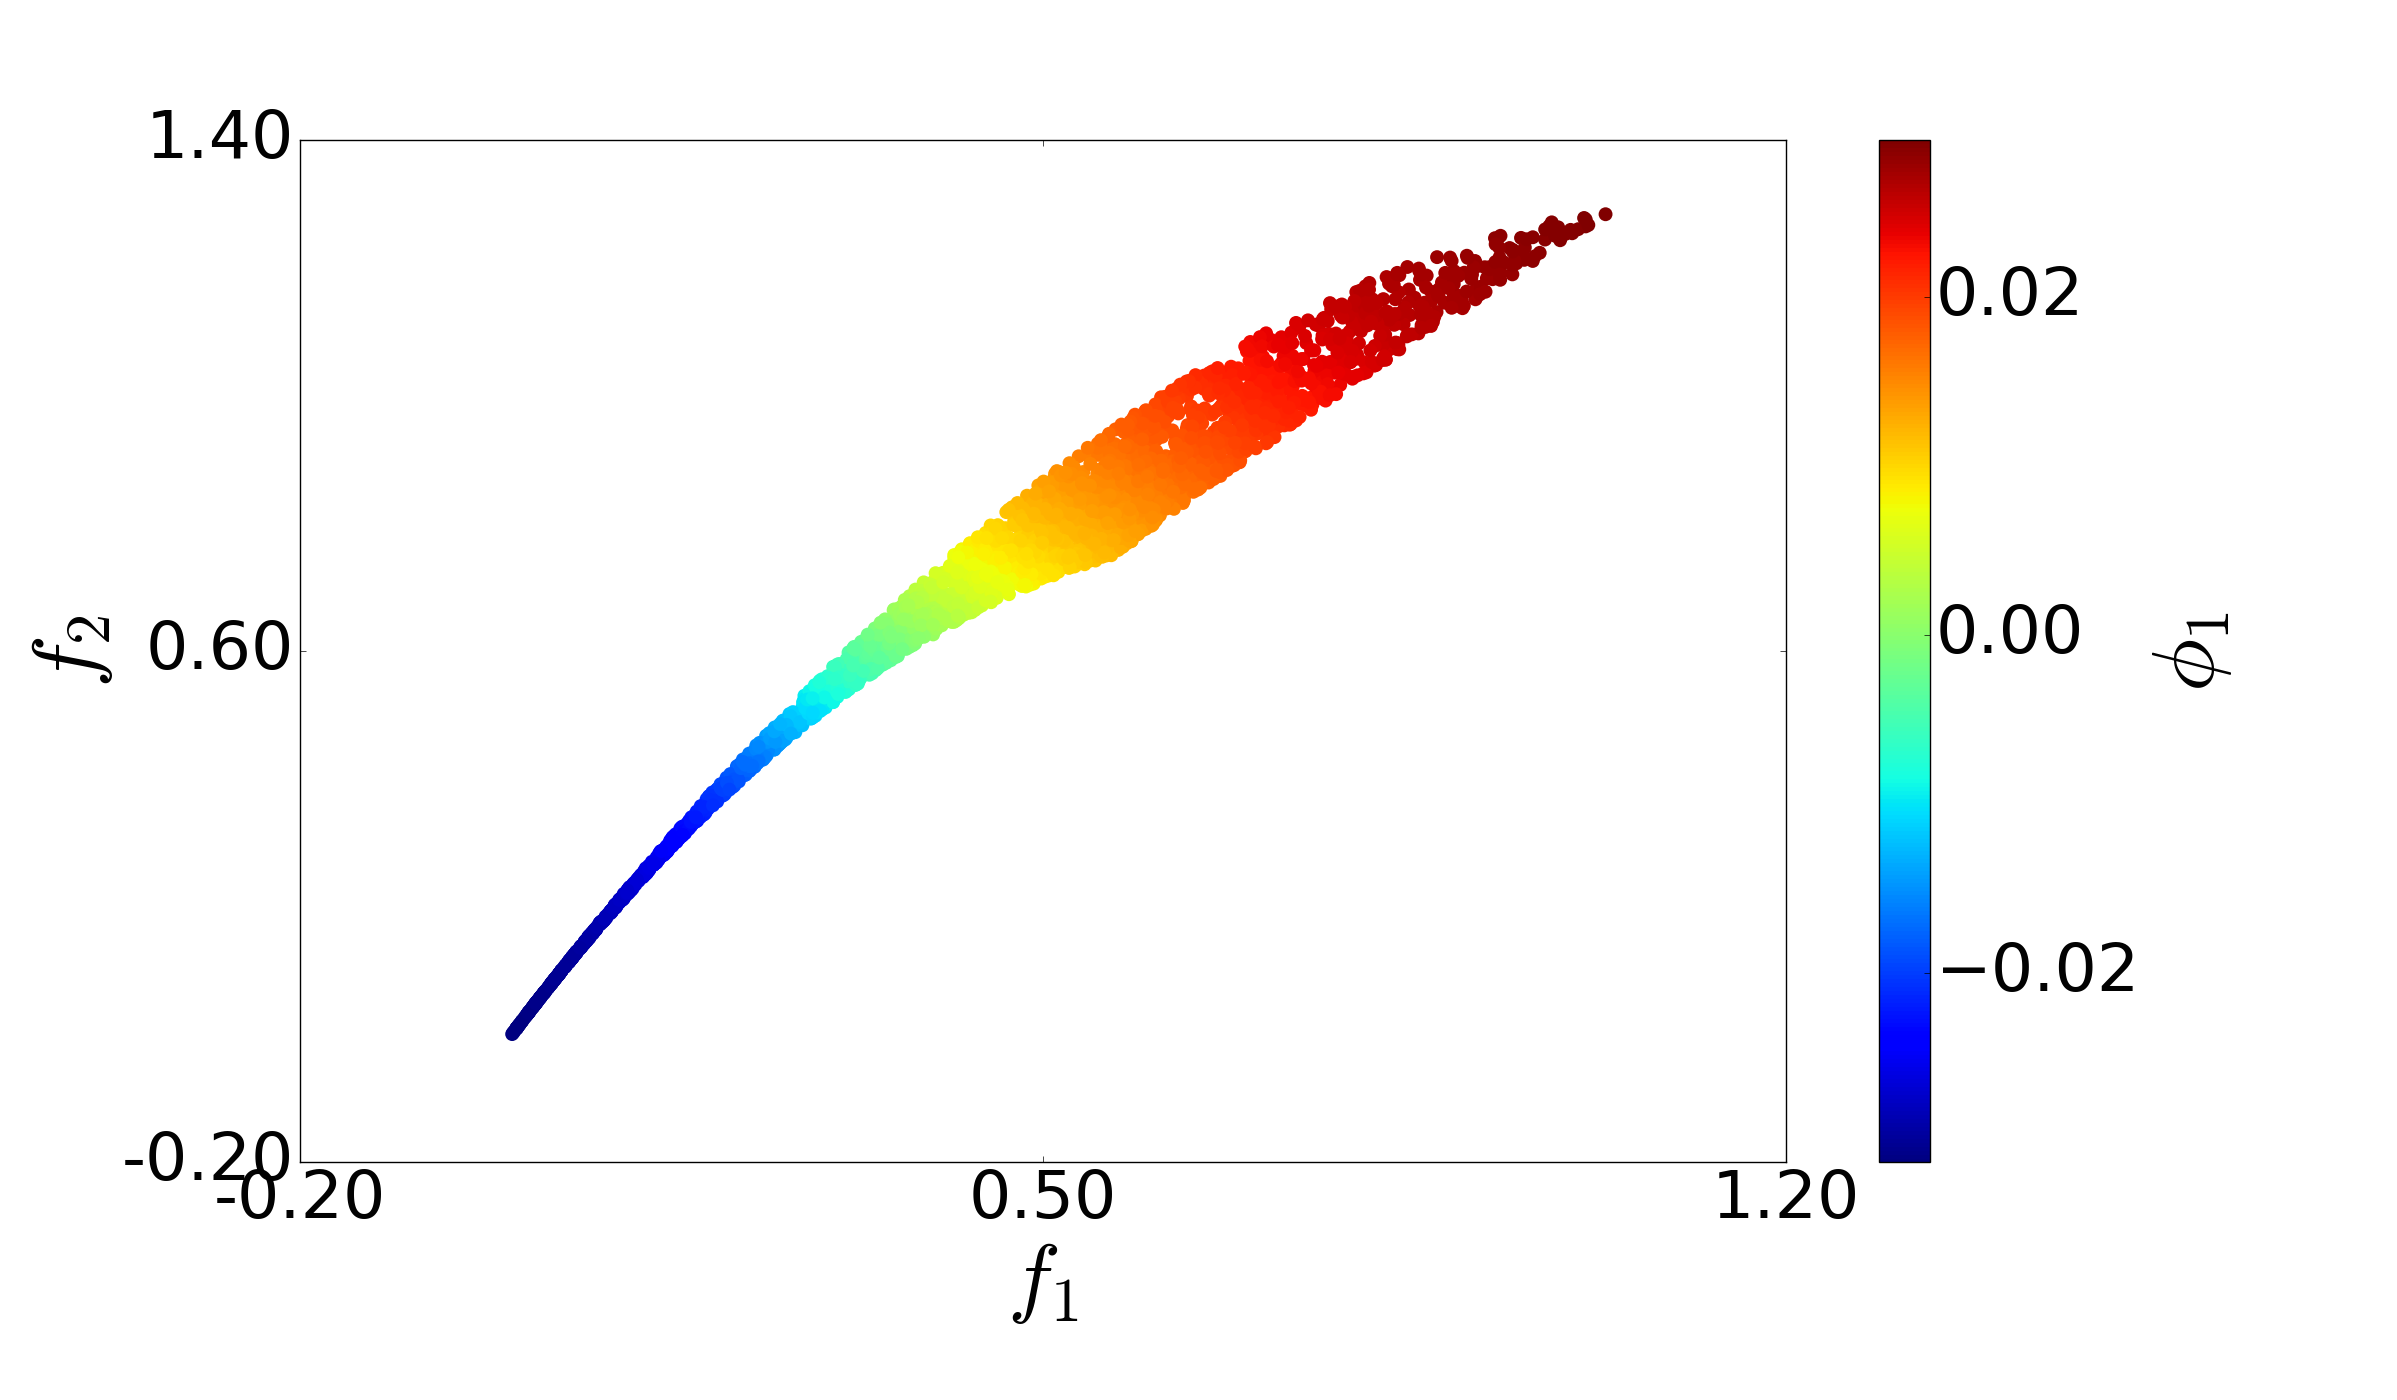
\includegraphics[width=1.0\linewidth]{f2-f1-phi1}
    \subcaption{Coloring the DMAPS embedding by $\epsilon$, revealing
      that indeed the two-dimensional region corresponds to large
      values of $\epsilon$, while the rest is singularly perturbed and
      one-dimensional.}
    % \subcaption{Coloring the model manifold by determinant of the
    % model response Jacobian, confirming that at large values the
    % system is two dimensional and not sloppy (red region) while at
    % small values the system is singularly perturbed and either one-
    % or two-dimensional (yellow to blue region).}
  \end{subfigure}
  \caption[Analysis of transformation from parameter space to the
    model manifold]{Analysis of transformation from parameter space to the
    model manifold. \label{fig:MM-ss} }
\end{figure*}

% \begin{figure*}
%   \centering
%   \begin{subfigure}[t]{0.45\linewidth}
%     \centering
%     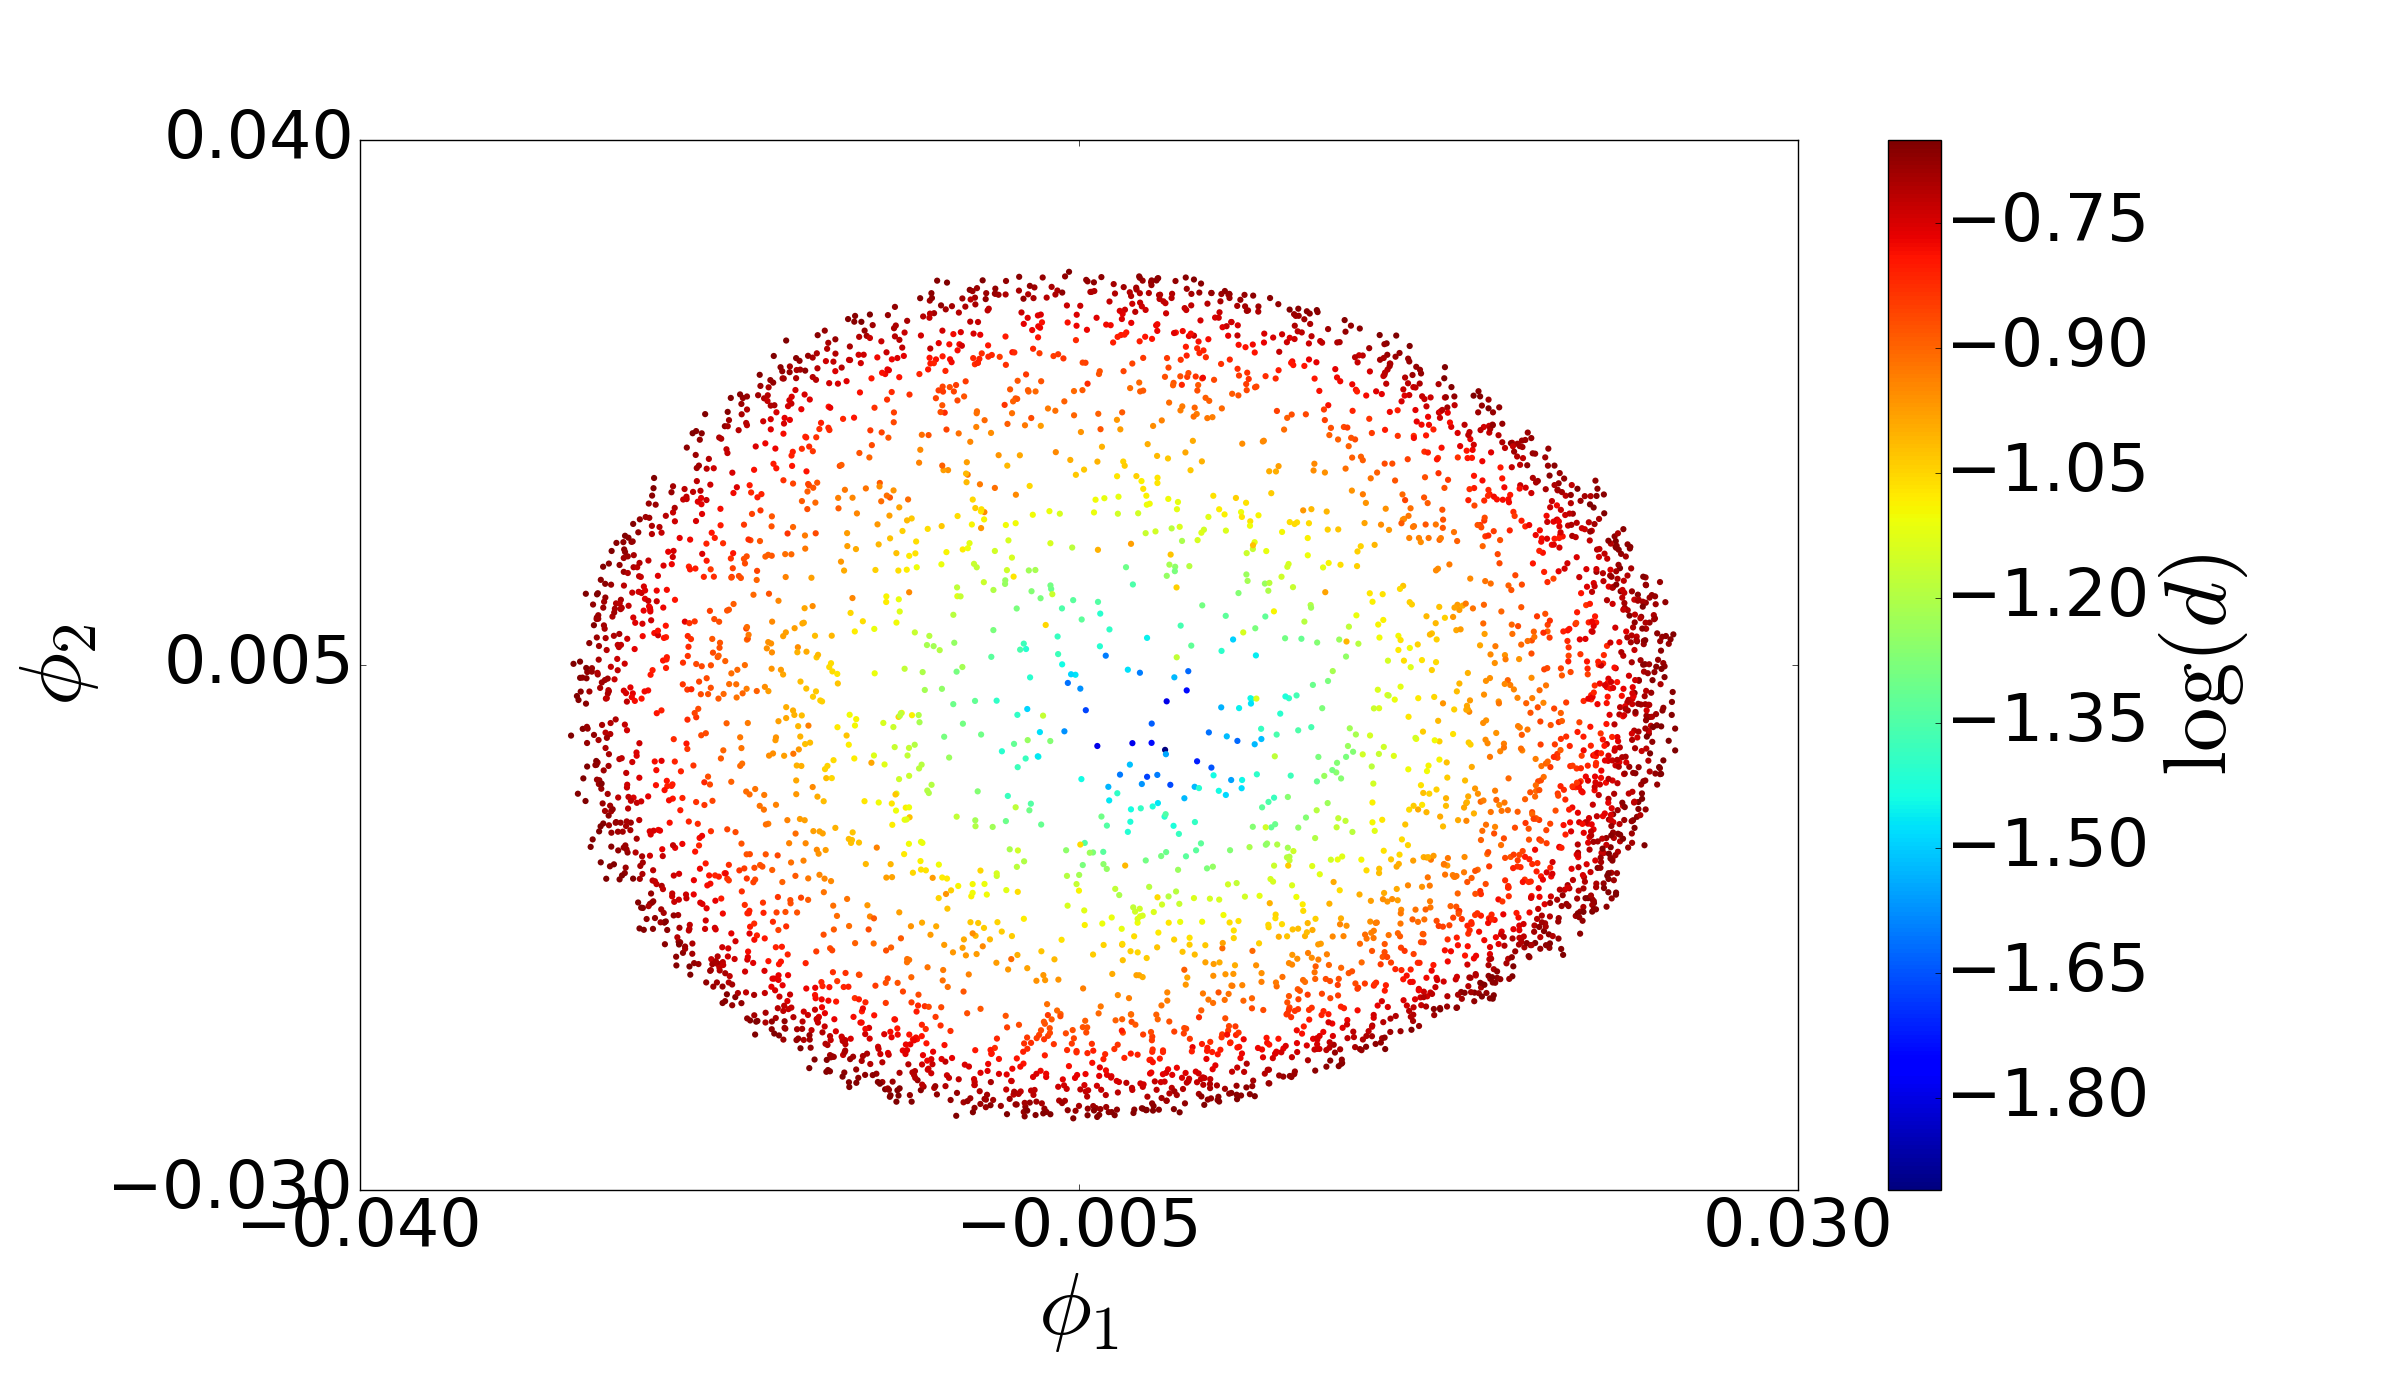
\includegraphics[width=1.0\linewidth]{phi2-phi1-d}
%     \subcaption{Coloring of two-dimensional DMAPS embedding in
%     $(\phi_1, \phi_2)$ by model response distance (i.e. the distance
%     between model output at two different sets of parameters). We
%     see that distance changes along both $\phi_1$ and $\phi_2$
%     suggesting that these eigenvectors parameterize significant
%     directions in parameter space.}
%   \end{subfigure}
%   \hspace{0.5cm}
%   \begin{subfigure}[t]{0.45\linewidth}
%     \centering
%     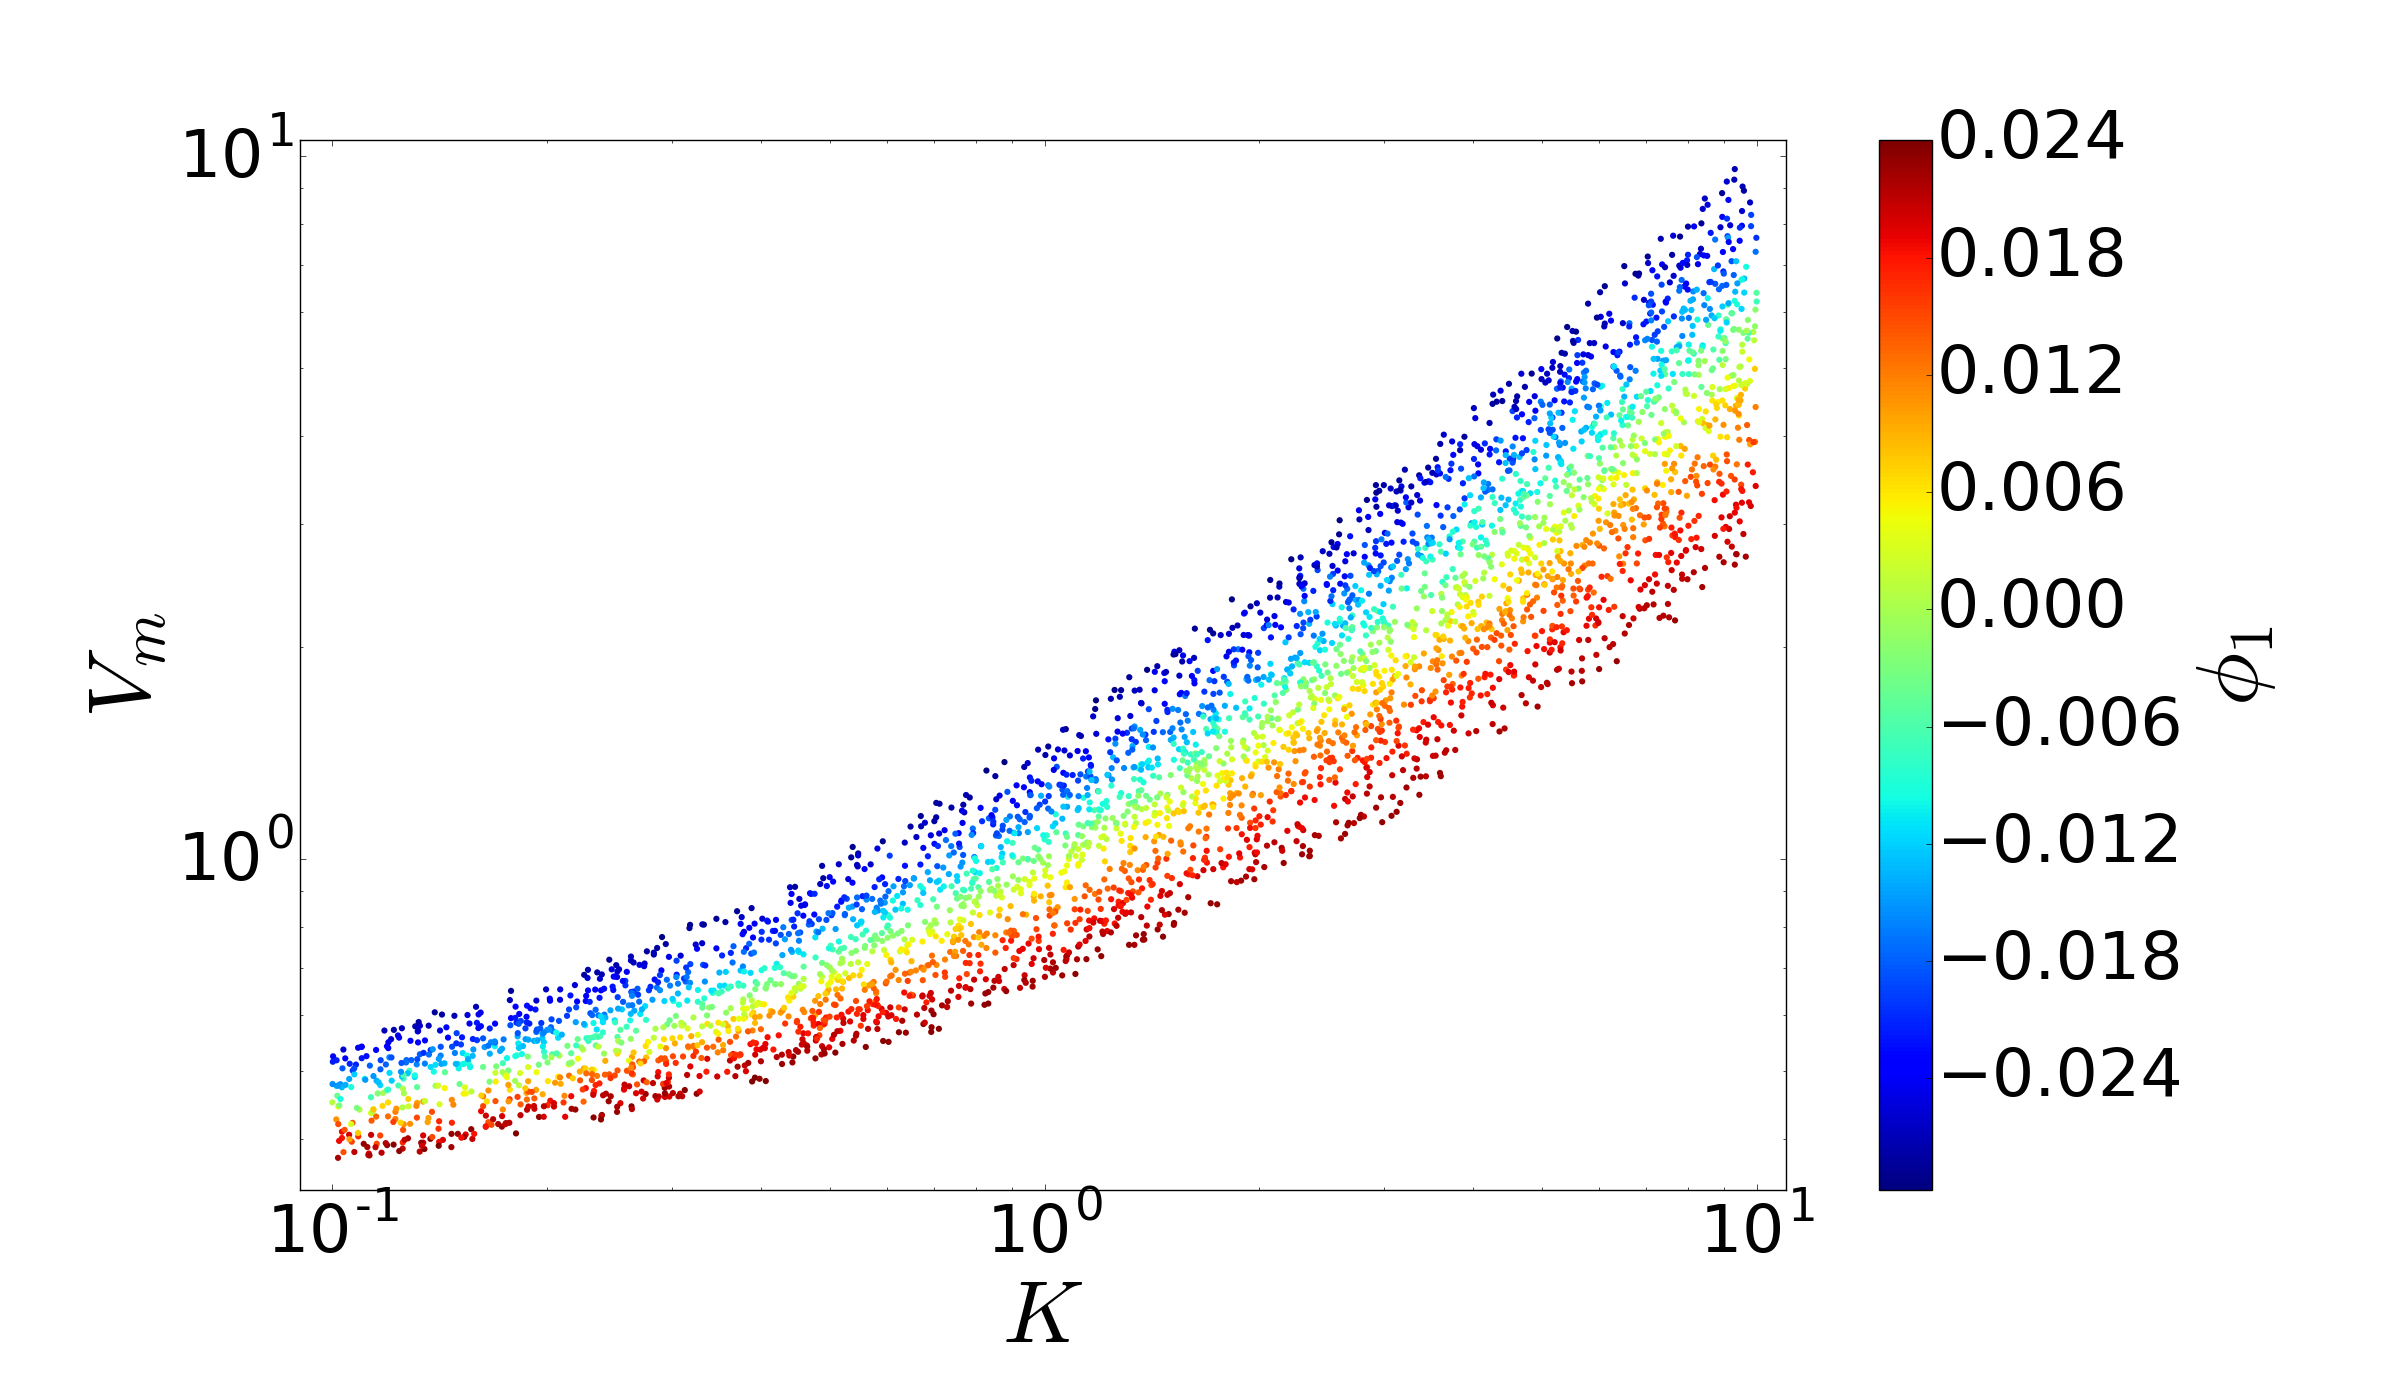
\includegraphics[width=1.0\linewidth]{v-k-phi1}
%     \subcaption{A projection of parameter space onto the $(K,V_m)$
%     plane and colored by the first DMAPS eigenvector. The color
%     changes along a direction orthogonal to contours of the sloppy
%     parameter $K/V$, showing that $\phi_1$ parameterizes a
%     significant direction as desired.}
%   \end{subfigure}
%   \caption{}
%   \label{fig:MM-ss}
% \end{figure*}

\begin{figure}
  \centering
  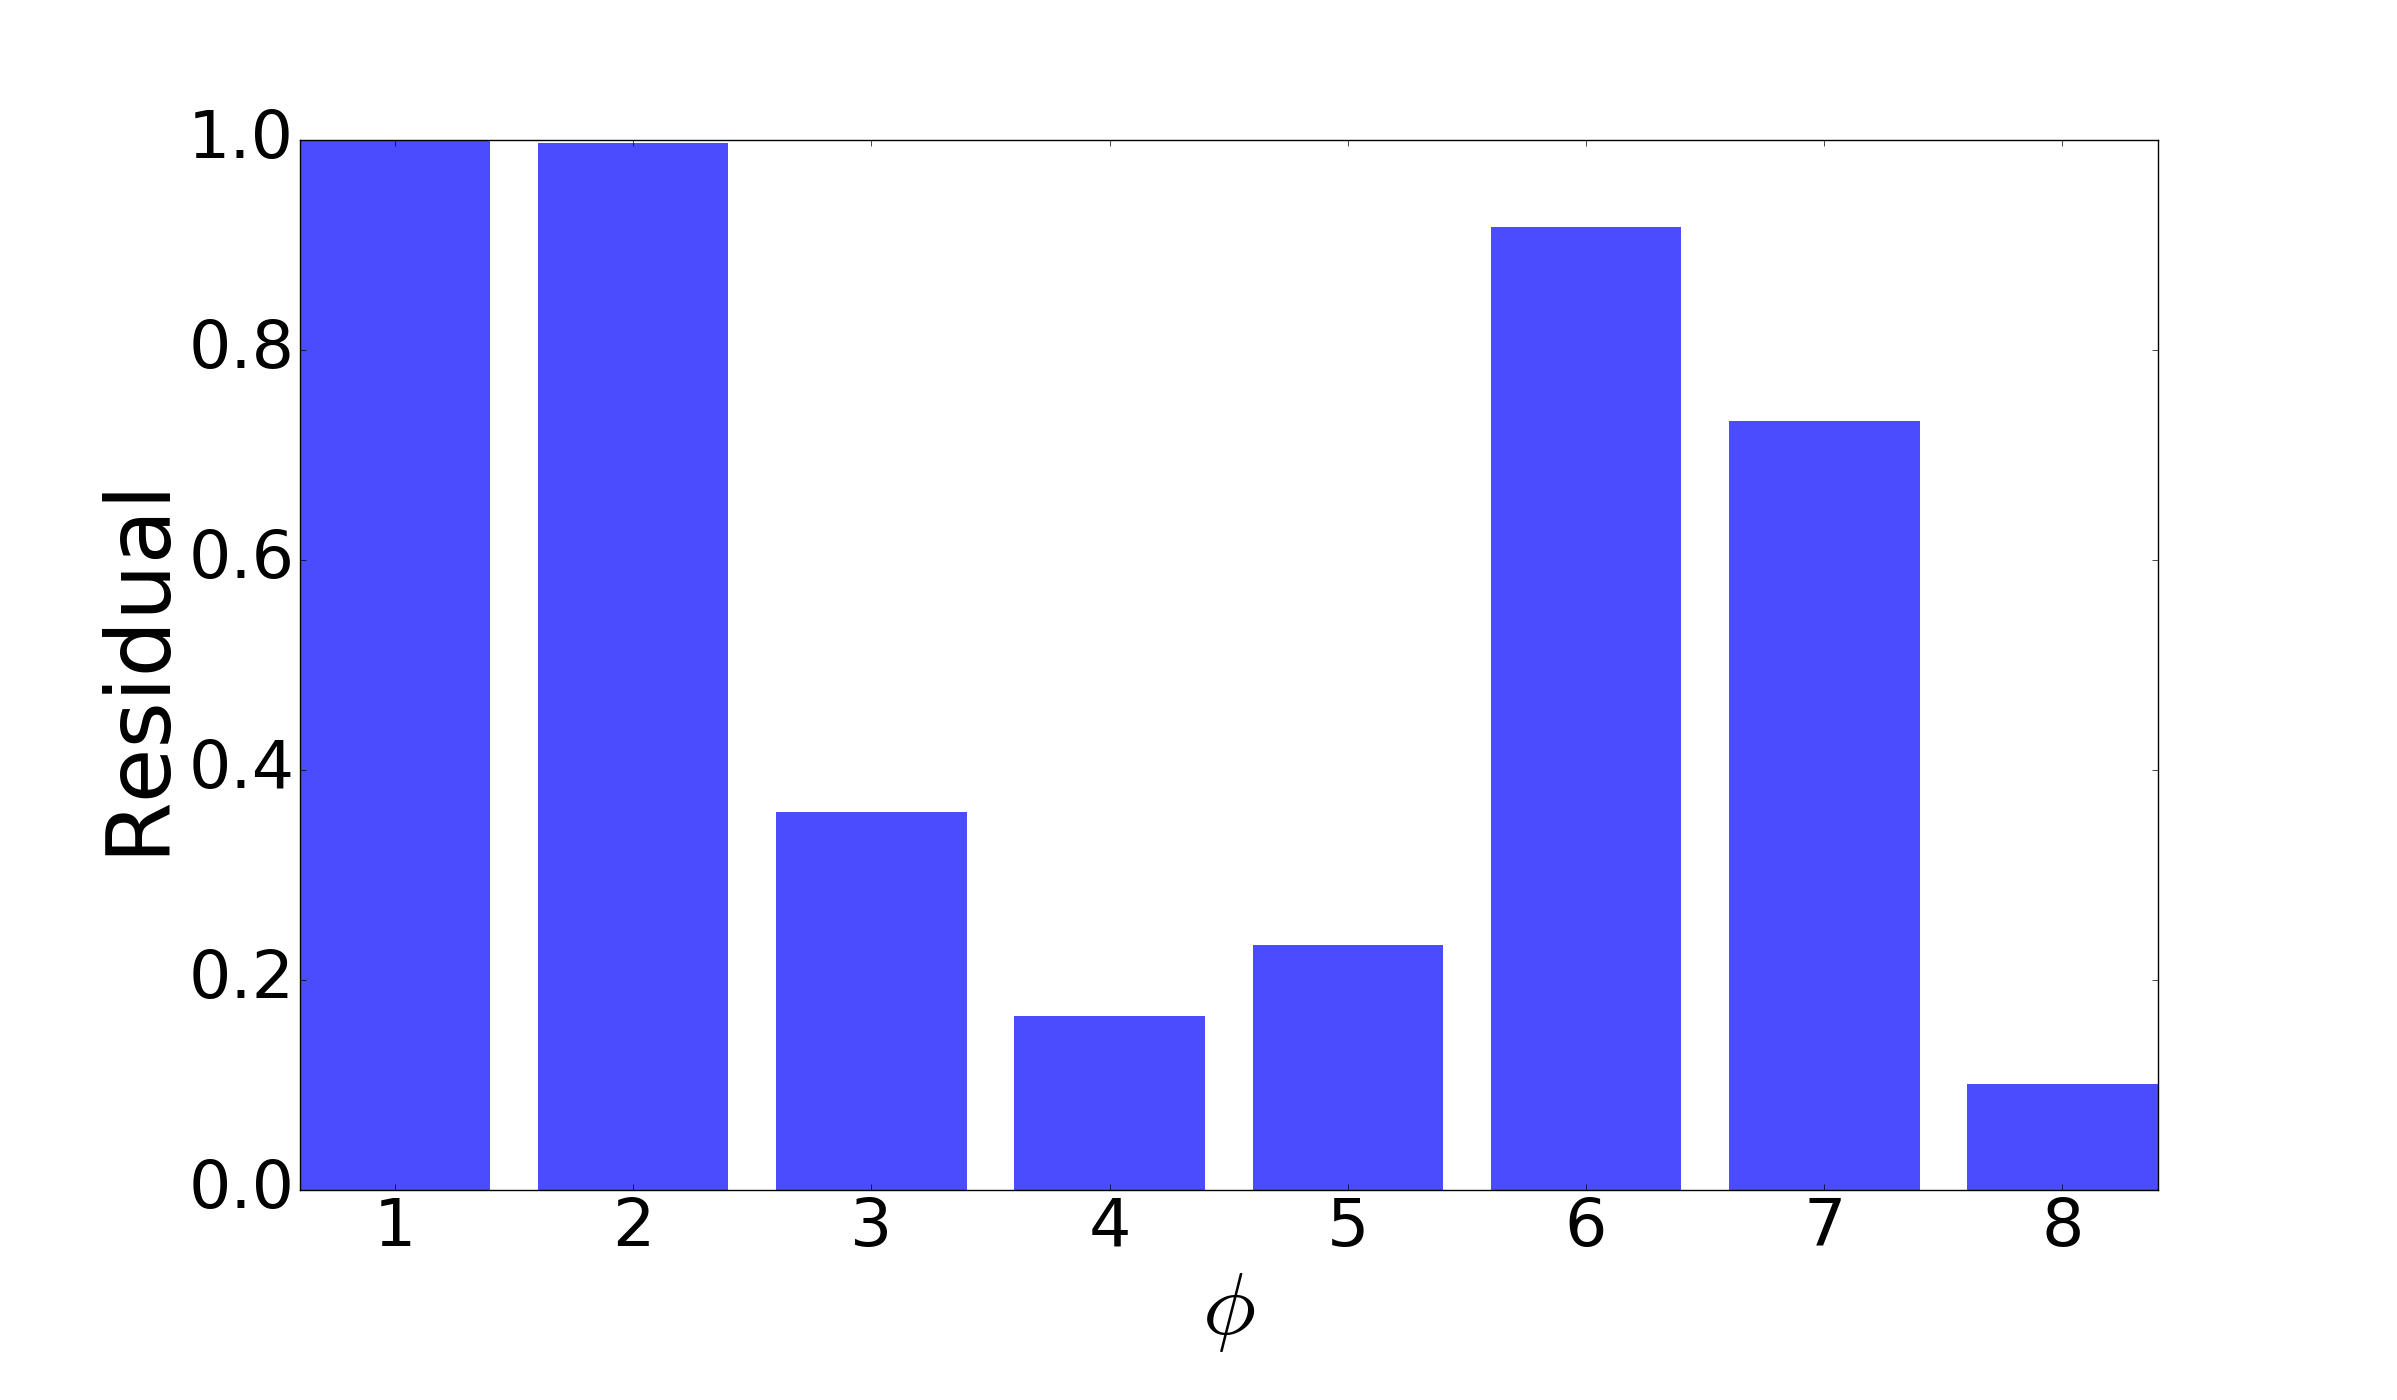
\includegraphics[width=1.0\linewidth]{residuals}
  \caption[Plot of DMAPS residuals showing which eigenvectors are
  independent]{Residuals computed as described in previous
    section. High residuals for a given eigenvector suggest that it is
    not a function of previous eigenvectors, and thus contains new
    information. This plot suggests five significant eigenvectors, the
    first two of which parameterize significant parameter directions,
    while the final three capture sloppy
    directions. \label{fig:resids} }
\end{figure}

% ------------------------------------------------

\section{Discussion}

By modifying the traditional DMAPS kernel to bias our random walks
along sloppy directions in parameter space, we have developed an
automated method of uncovering nonlinear effective parameters in
complex models. Future work will focus on using these embeddings to
accelerate optimization in these settings, where simple gradient
descent based techniques often become trapped in sloppy regions of
parameter space and converge slowly.
